\documentclass[12pt, letterpaper]{article}
\usepackage{times}
\usepackage{graphicx}
\usepackage{import}
\usepackage{fancyhdr}
\usepackage{wrapfig}
\usepackage[utf8]{inputenc}
\usepackage[hidelinks]{hyperref}
\usepackage{subcaption}
\usepackage{pdfpages}
\usepackage{enumitem}
\usepackage{titling}
\pagestyle{fancyplain}% <- use fancyplain instead fancy
\fancyhf{}
\addtolength{\headheight}{15pt}
\fancyhead[L]{Cyber Security: PSP - Konstantinos Poumpouridis}% <- added
\fancyhead[R]{488394}
\fancyfoot[C]{\thepage}
%\renewcommand\headrulewidth{0pt}% default ist .4pt
\renewcommand{\plainheadrulewidth}{.4pt}% default is 0pt
\title{Personal Specialisation Project: Hackintosh}
\author{Konstantinos Poumpouridis}
\date{11/05/2023}
\pagenumbering{arabic}
% set up \maketitle to accept a new item
\predate{\begin{center}\placetitlepicture\large}
\postdate{\par\end{center}}

% commands for including the picture
\newcommand{\titlepicture}[2][]{%
  \renewcommand\placetitlepicture{%
    \includegraphics[#1]{#2}\par\medskip
  }%
}
\newcommand{\placetitlepicture}{} % initialization
\begin{document}
\titlepicture[width=0.6\textwidth]{fotos/PSP/Hackintosh title.jpeg}
\maketitle
\thispagestyle{empty}
\newpage
\section{Changelog}
    \begin{table}[htbp]
        \begin{tabular}{|l|l|l|}
            \hline
            Version & Changes         & Date   \tabularnewline \hline
            0.1     & Initial version & 11/05/23 \tabularnewline \hline
            0.2     & Added text and added  & 23/05/23 \tabularnewline \hline
            0.3     & Some changes to the questions & 30/05/23 \tabularnewline \hline
            0.4     & Some changes to 6.1 and reworked questions & 07/06/23 \tabularnewline \hline
            0.5     & Removed History  & 13/06/23 \tabularnewline \hline
            0.6     & Finishing up my document  & 14/06/23 \tabularnewline \hline
            0.7     & Reworked my document  & 16/06/23 \tabularnewline \hline
        \end{tabular}
    \end{table}
\newpage
\tableofcontents
\newpage

\section{Introduction}
People wanted to have MacOS without buying Mac devices. So once Apple left IBM PowerPC chips the flood of hackers went In and try to port it to other non-Apple devices to see run it as daily drivers. That's how Hackintosh was born.

\section{Background}
Since 2015 when Apple switched from PowerPC to Intel-based Macs which open the possibilities for porting MacOS to non-based Macs. It started with Mac OS X Tiger (10.4).

%\subsection{History}
 

% \subsubsection{Mac OS X Tiger (10.4)}
% On June 6 2015 Apple announced that it would support X86 architecture with Intel. So it was the first version that supported x86 execution. This was also the first time that they support EFI which most of the other brands still ran on old legacy BIOS. The hackers managed to make it run on SSE 3 CPU's which means a Pentium 4 (SSE 2) has limited instructions but it was a promising start.
% \subsubsection{Mac OS X Leopard (10.5)}


% \subsubsection{Mac OS X Snow Leopard (10.6)}

% \subsubsection{Mac OS X Lion (10.7)}

% \subsubsection{Mac OS X Mountain Lion (10.8)}

% \subsubsection{OS X Mavericks (10.9}

% \subsubsection{OS X Yosemite (10.10)}

% \subsubsection{OS X El Capitan (10.11)}

% \subsubsection{macOS Sierra (10.12)}
% This version has hackers-created AMD Processors support

% \subsubsection{macOS High Sierra (10.13}

% \subsubsection{macOS Mojave (10.14)}

% \subsubsection{macOS Catalina (10.15)}

% \subsubsection{macOS Big Sur (11)}

% \subsubsection{macOS Monterey (12)}

% \subsubsection{macOS Ventura (13)}

\newpage

\section{Objectives}
The main objectives of this investigation are:
\begin{itemize}
    \item To make macOS run on non-apple devices.
\end{itemize}
\section{Project scope}
\subsection{Within the scope}
\begin{itemize}
    \item Altering Laptop software wise
    \item Costing no money
    
\end{itemize}
\subsection{Outside the scope}
\begin{itemize}
    \item If it cost money
    \item If the project takes more than 60hr
\end{itemize}
\newpage
\section{Methodology}
The investigation was conducted using a combination of manual and automated techniques. The following steps were taken:
\hfill\break
\hfill\break
Since this is offensive hacking this means we are going to modify our EFI (bootloader) into tricking our system to run the unmodified macOS

\subsection{Native Hackintosh}
With a native Hackintosh, you must follow the Clover or OpenCore guide. After researching on Reddit, Olarila forums and tonymacx86. So the method is to use OpenCore Efi and It was recommended to use Intel-based to be most compatible.
\hfill\break
\hfill\break
OpenCore helps us spoof our system to run macOS so what it does is convince the macOS.
\hfill\break
\hfill\break
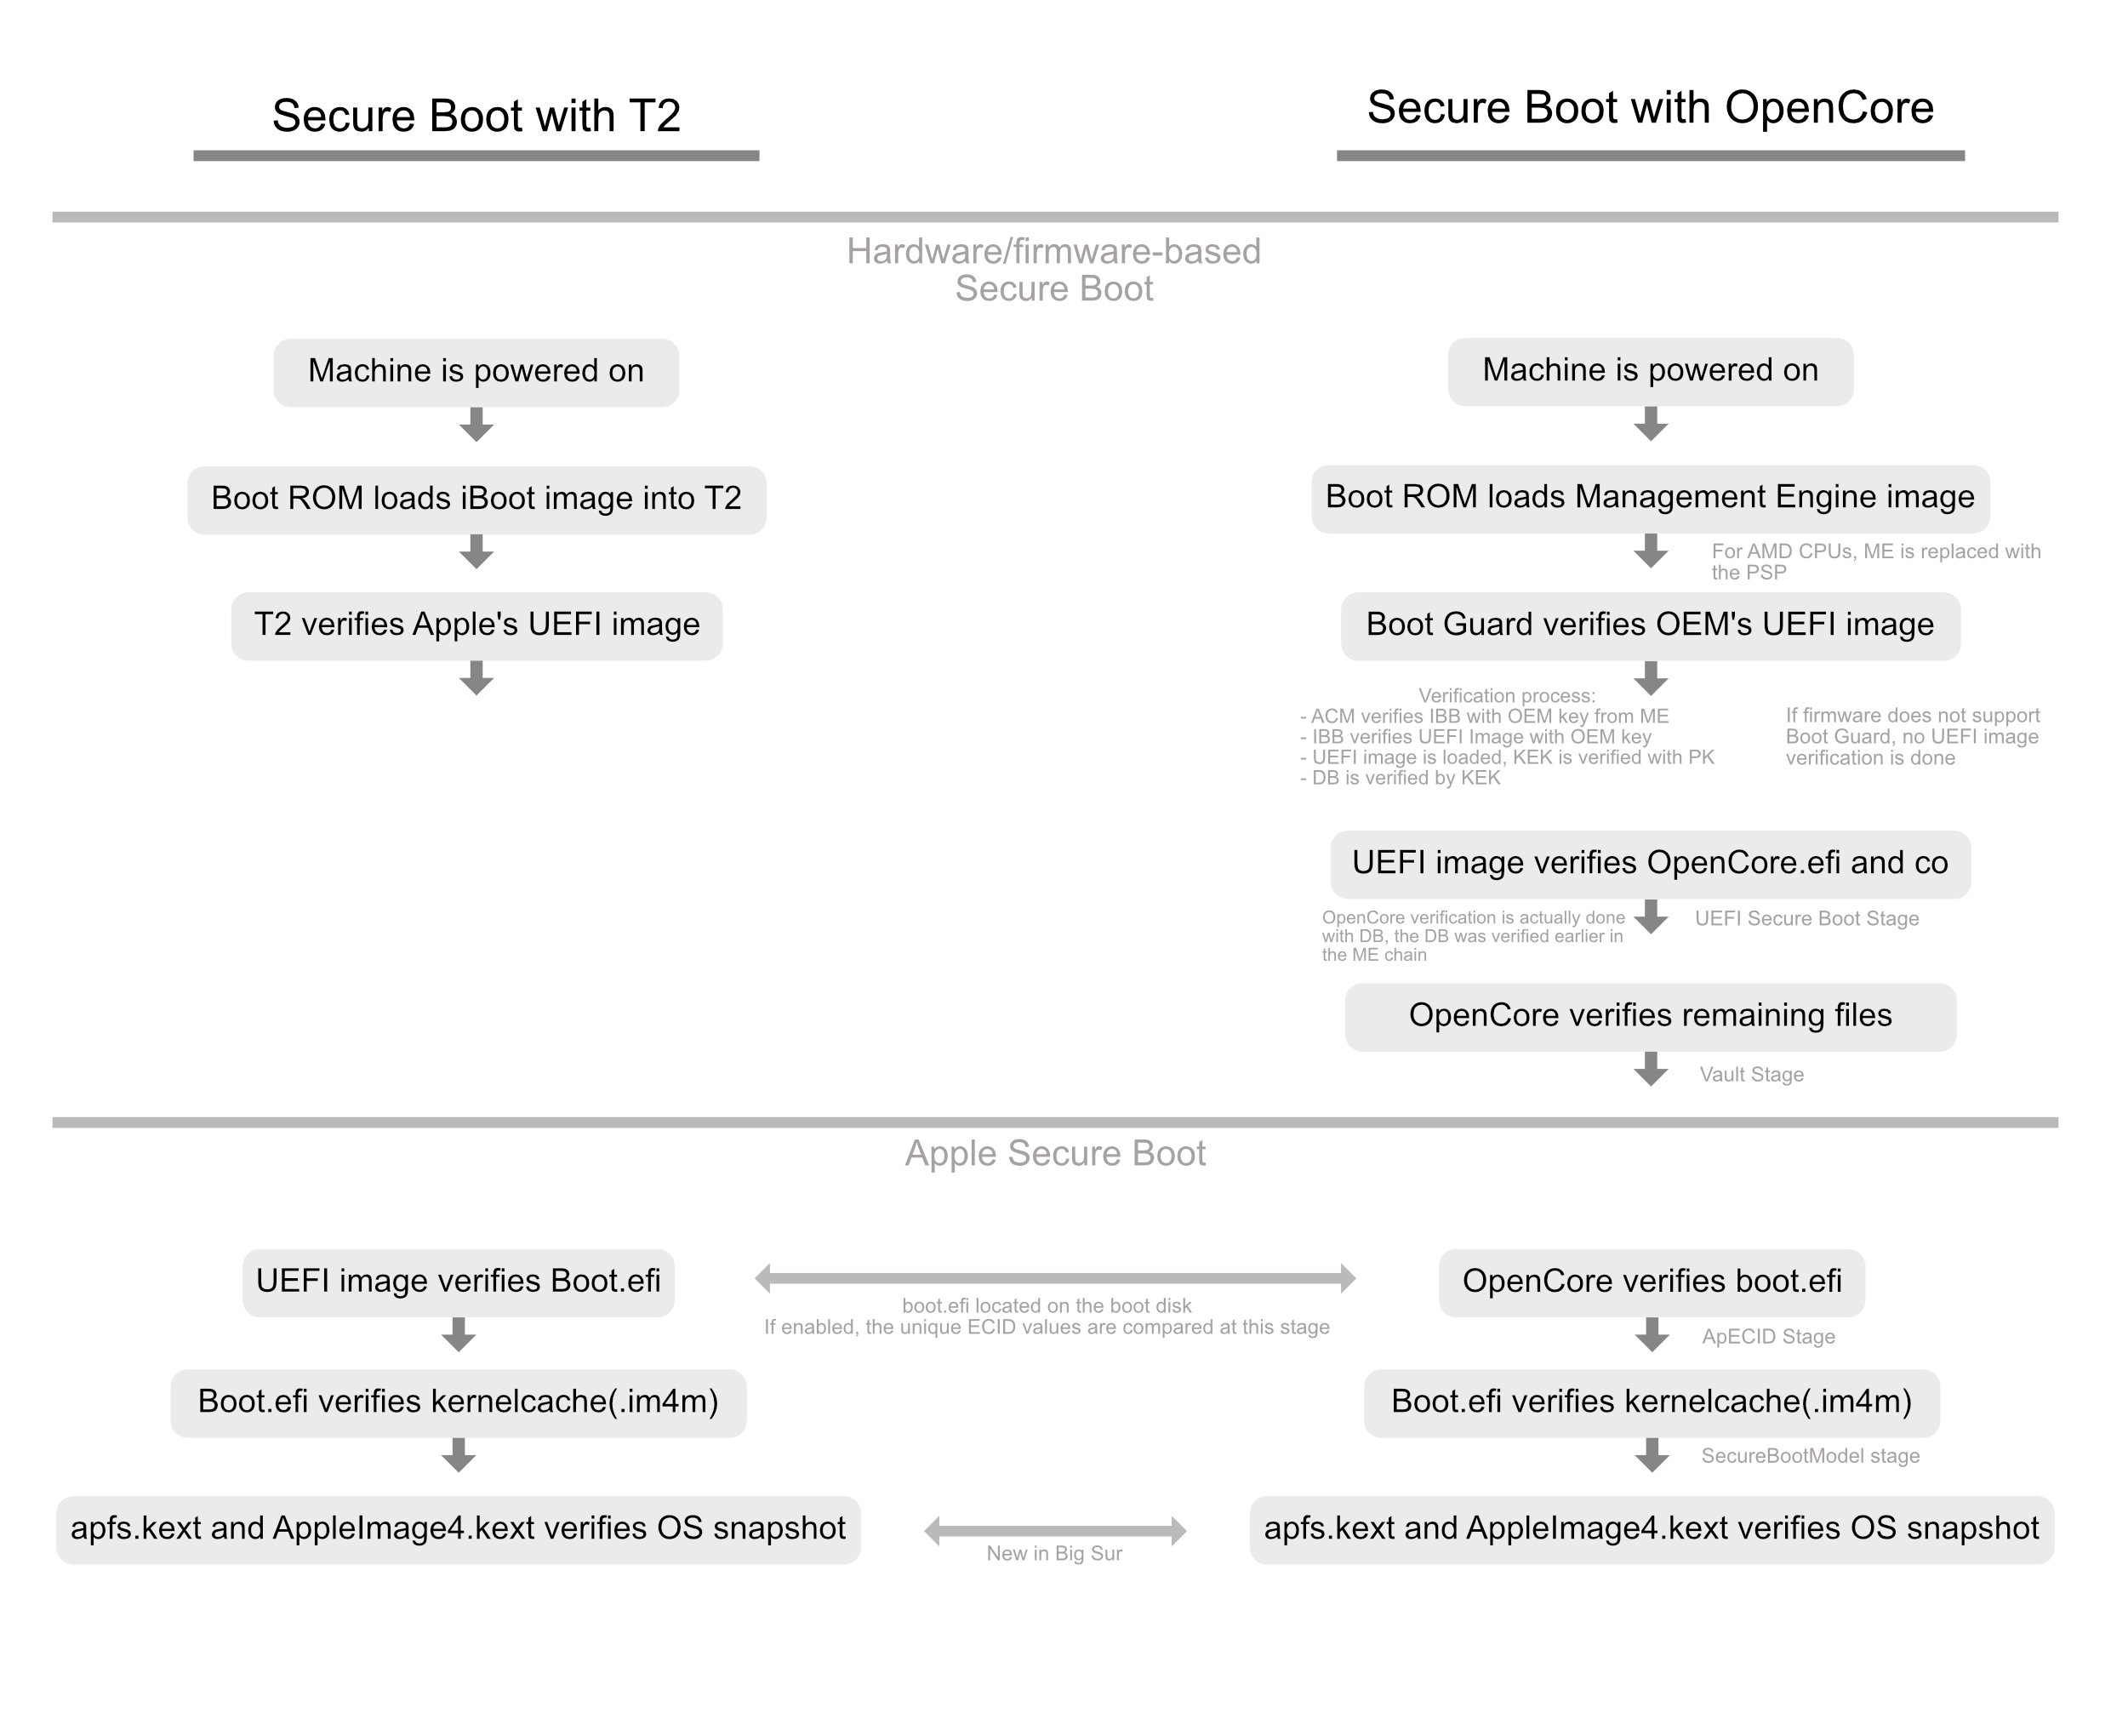
\includegraphics[width=0.9\textwidth]{fotos/PSP/Research/Native/Opencore Erik tekening.png}

\hfill\break
\hfill\break
\textbf{In order to run you need to have these requirements.}
\subsubsection{CPU}
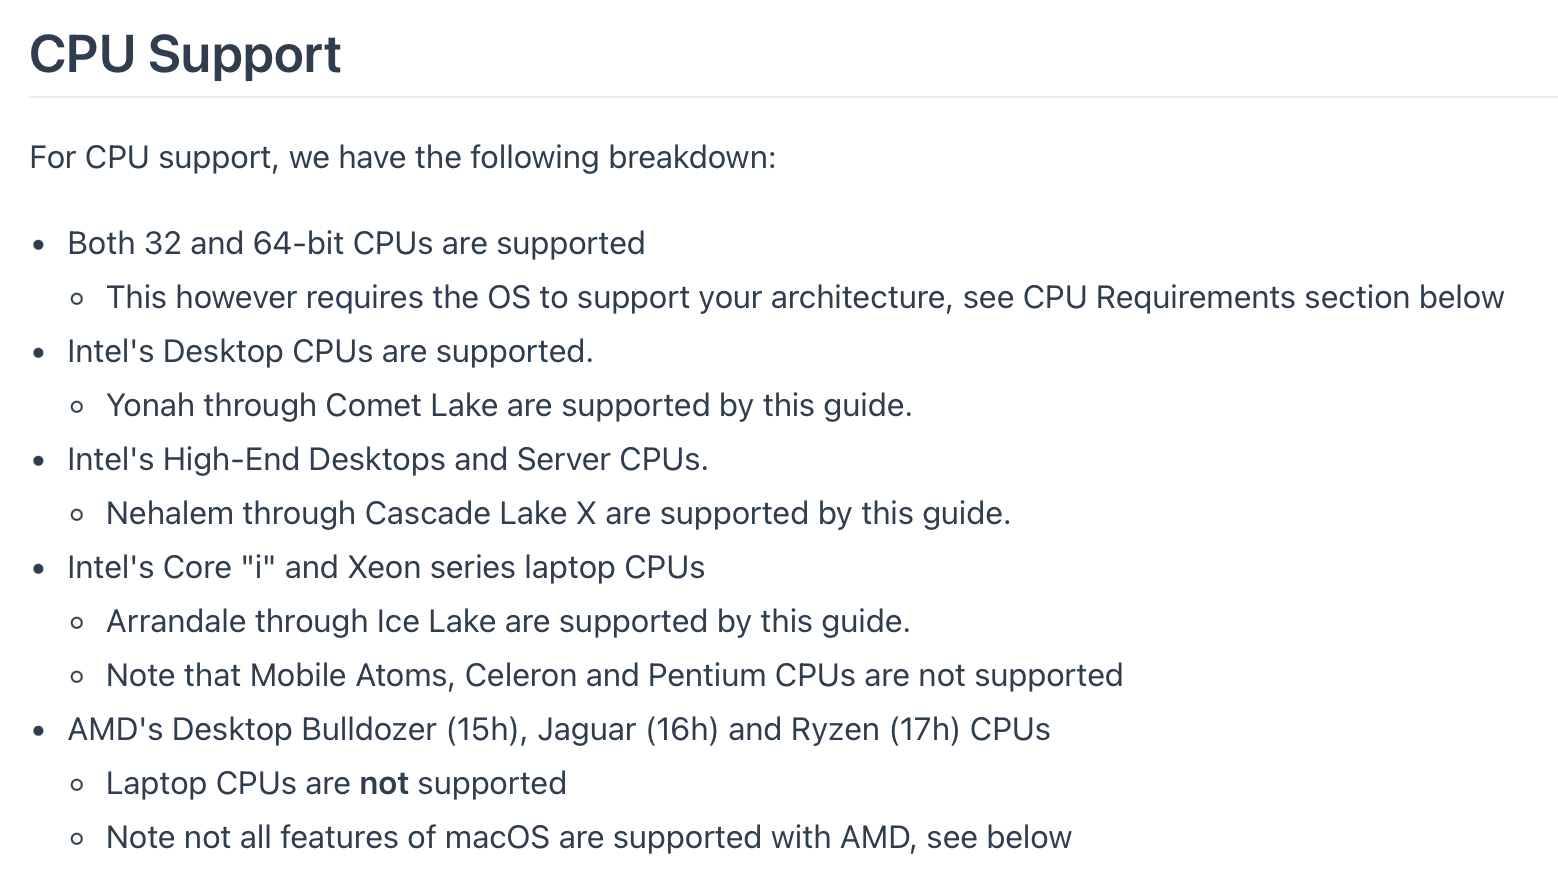
\includegraphics[width=0.8\textwidth]{fotos/PSP/Research/Native/Open core req cpu.jpeg}
\break
\emph{dortania.github.io CPU requirements}
\hfill\break
\hfill\break
The best support is to use Intel because AMD can be finicky. It is better to use 11th gen or lower. The best option is to be close to the real counterparts.
\hfill\break
\hfill\break
\subsubsection{GPU}
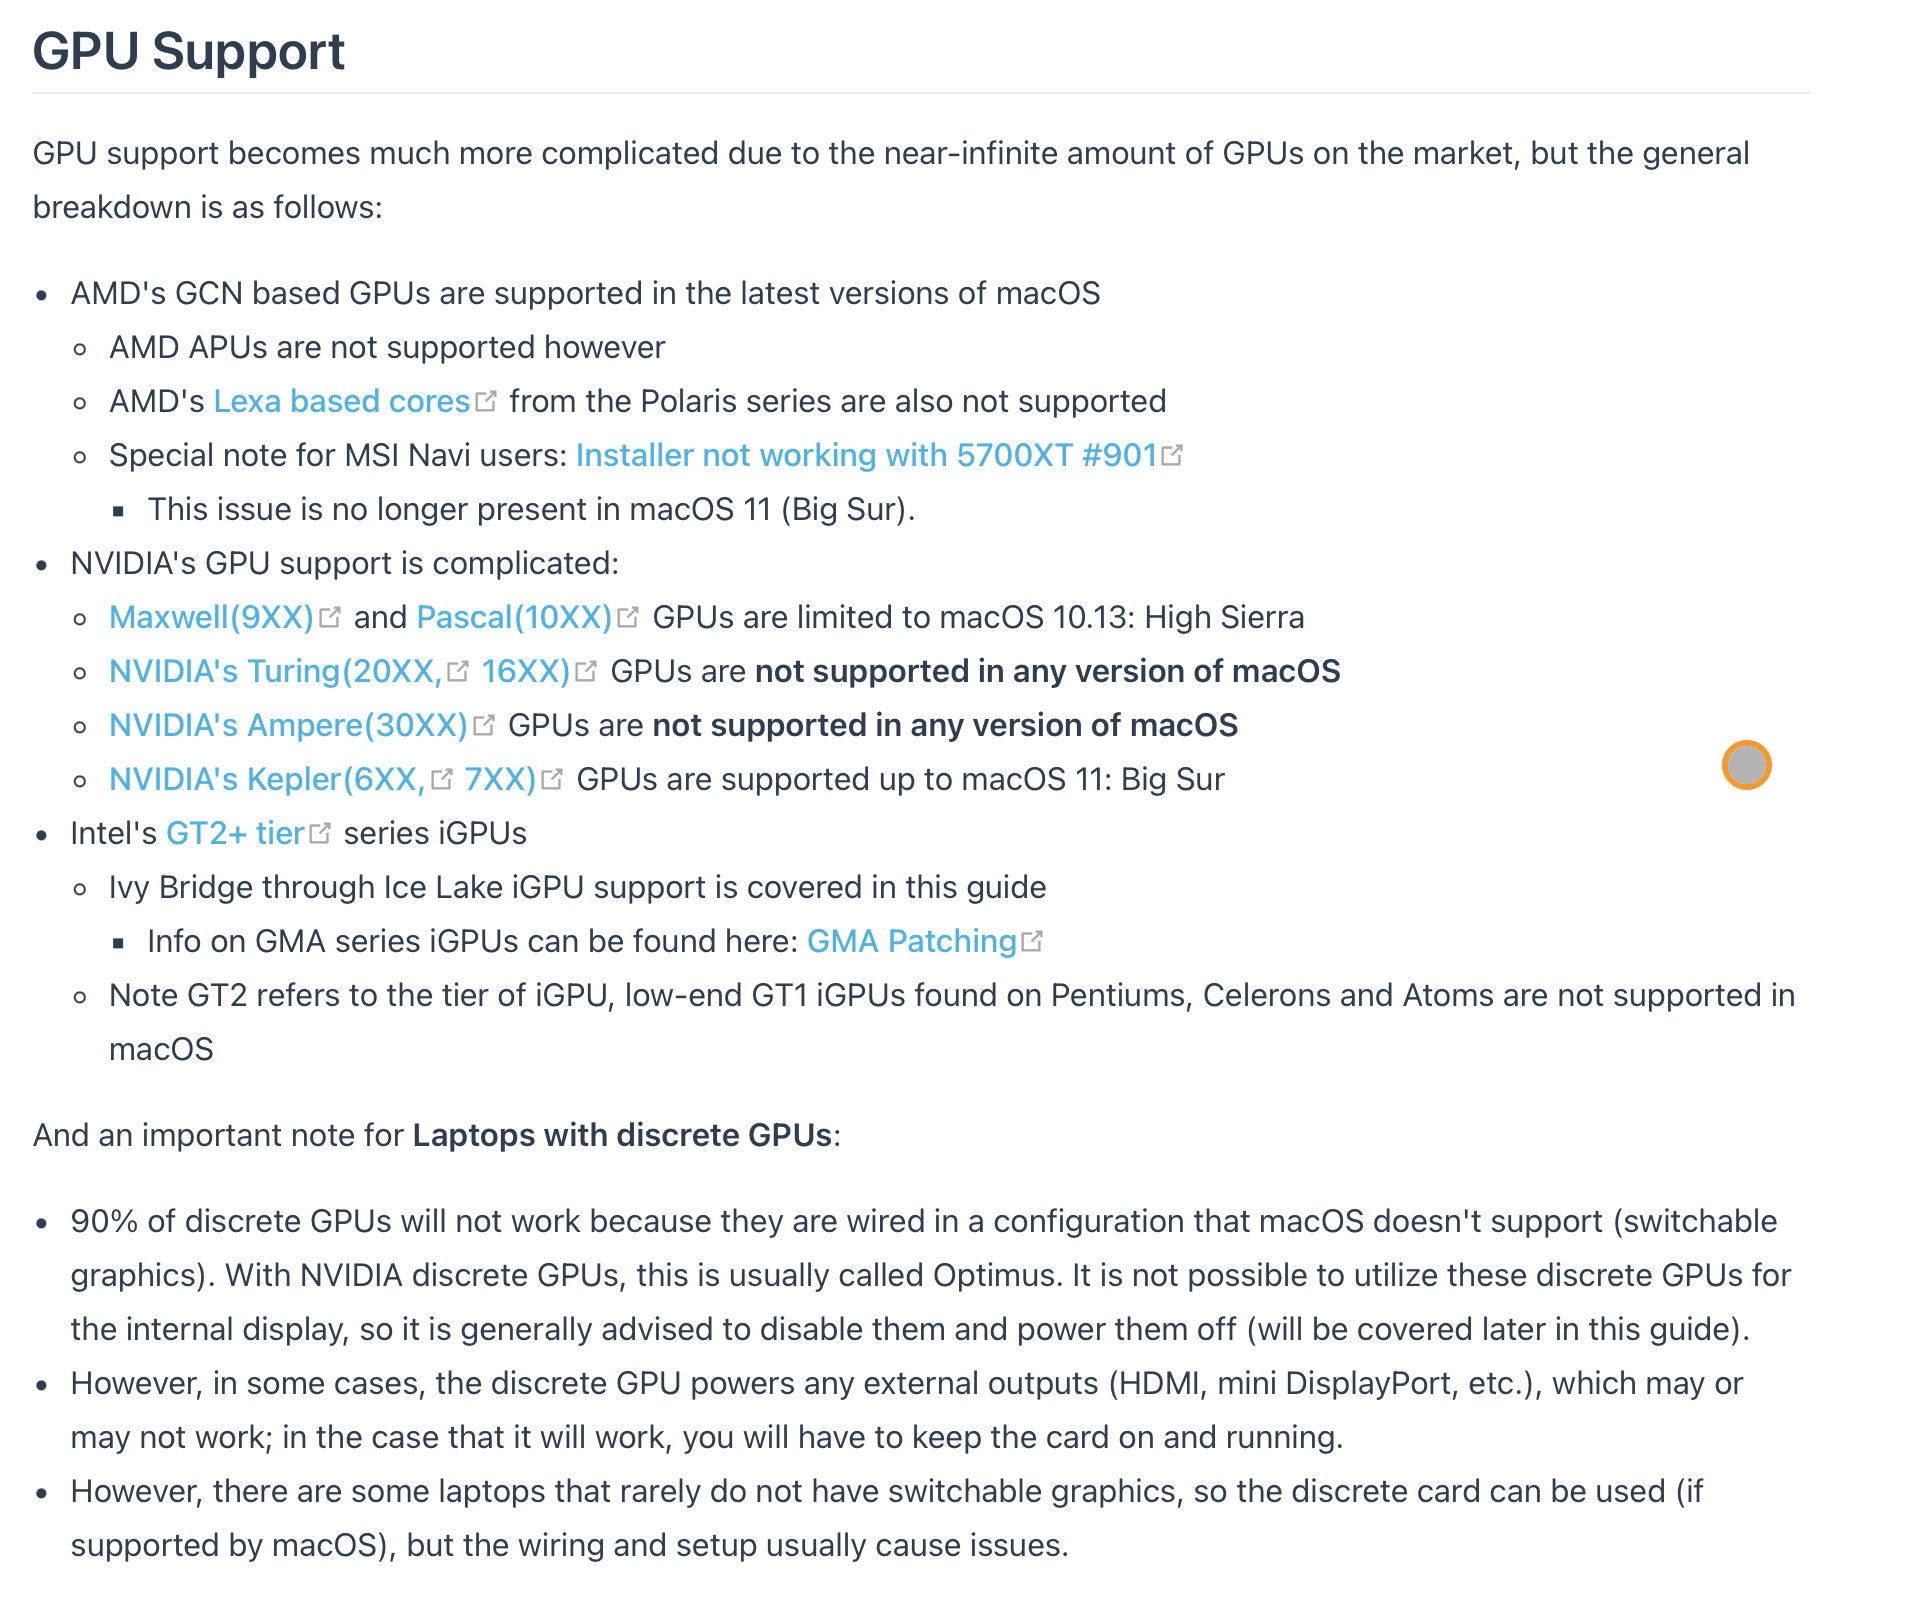
\includegraphics[width=0.8\textwidth]{fotos/PSP/Research/Native/Open core req gpu.jpeg}
\break
\emph{GPU requirements}
\hfill\break
\hfill\break
For modern macOS, we would recommend running on Intel graphics since this offers the best compatibility but if you want some raw power them some AMD cards are compatible with Metal 3 support. We only recommend 
\hfill\break
\hfill\break
\subsubsection{Network}
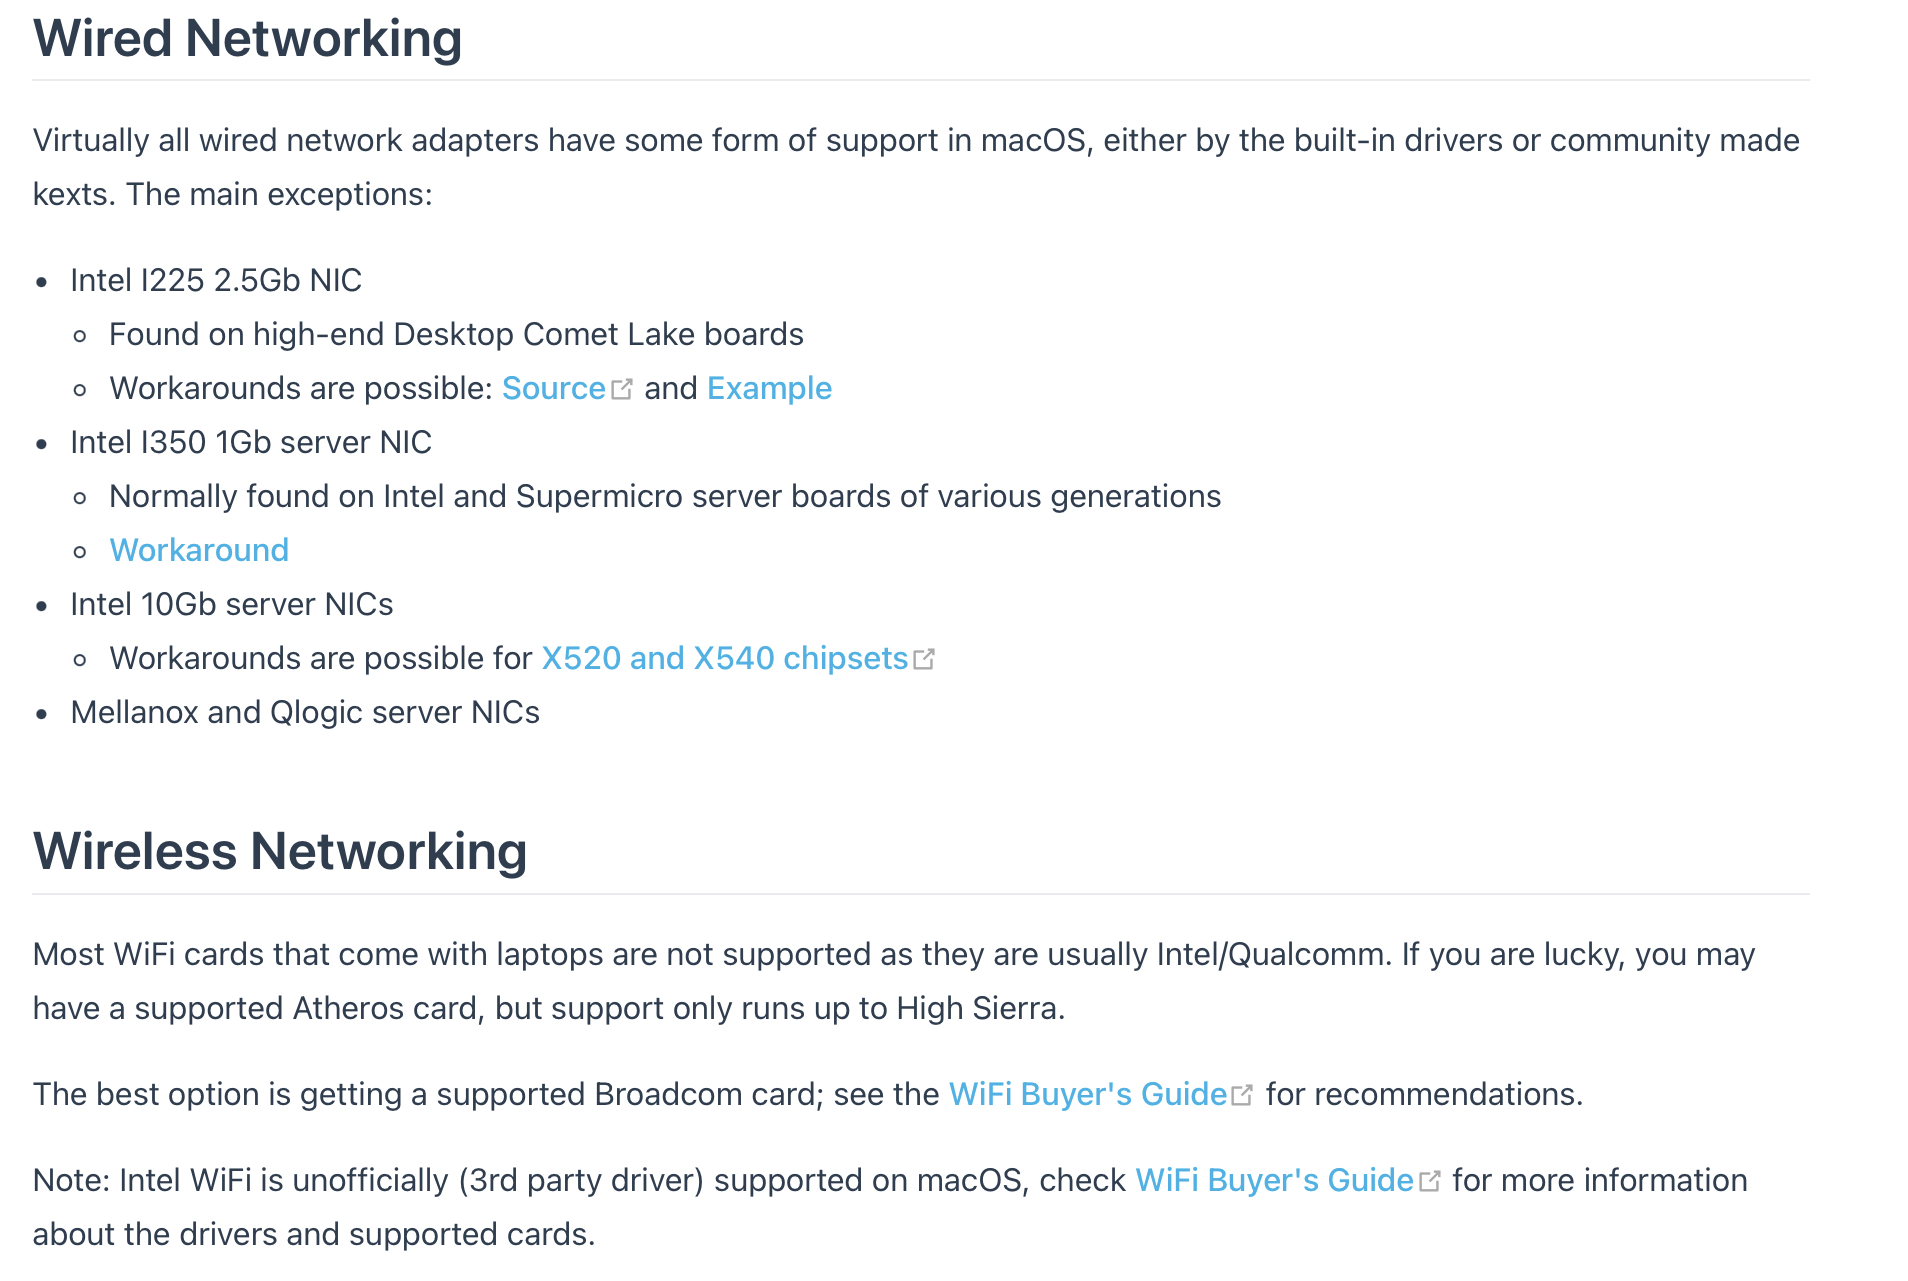
\includegraphics[width=0.8\textwidth]{fotos/PSP/Research/Native/Open core req network.jpeg}
\break
\emph{Requirements for network}
\hfill\break
\hfill\break
Most Broadcom and Intel networks should work fine.
\newpage
\subsubsection{Storage}
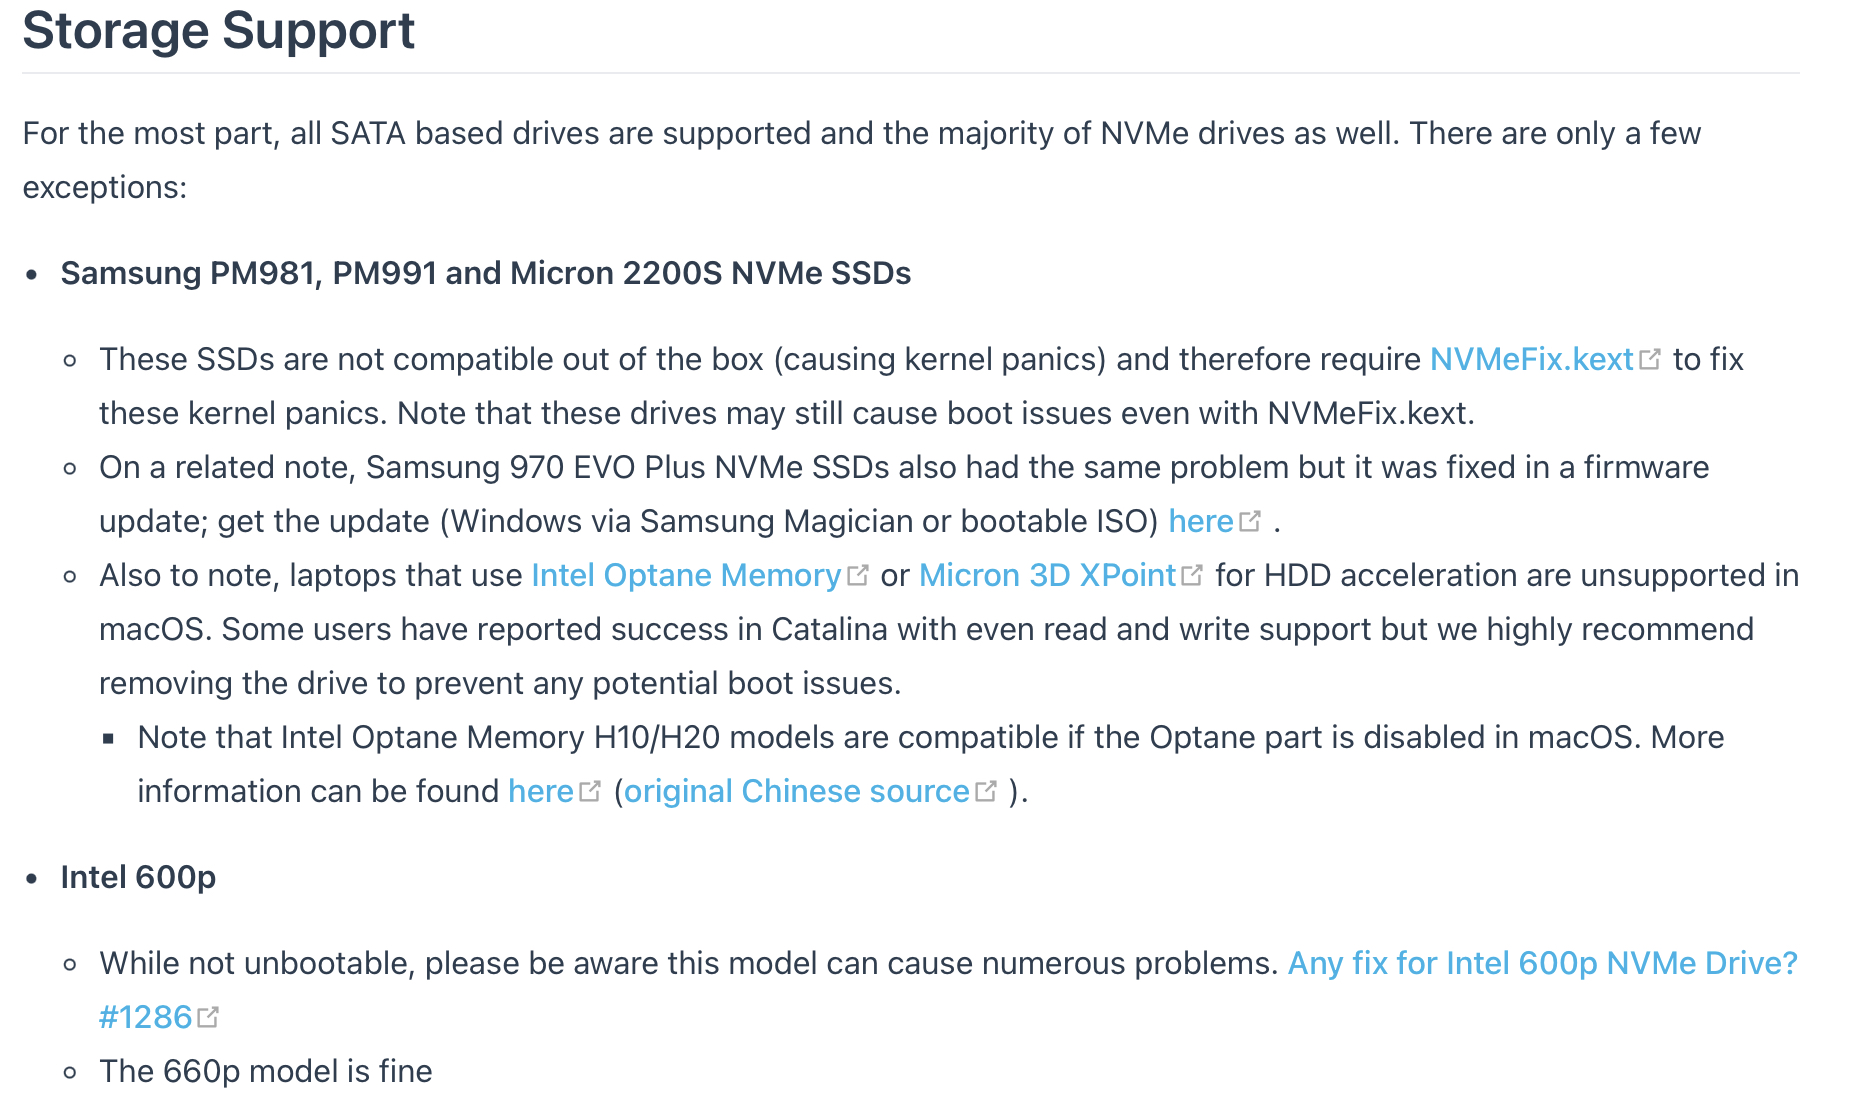
\includegraphics[width=0.8\textwidth]{fotos/PSP/Research/Native/Open core req storage.jpeg}
\break
\emph{Storage requirement}
\hfill\break
\hfill\break
It works fine but there is an issue with Samsung 970 old series.
\hfill\break
\hfill\break
\newpage
\subsubsection{Misc}
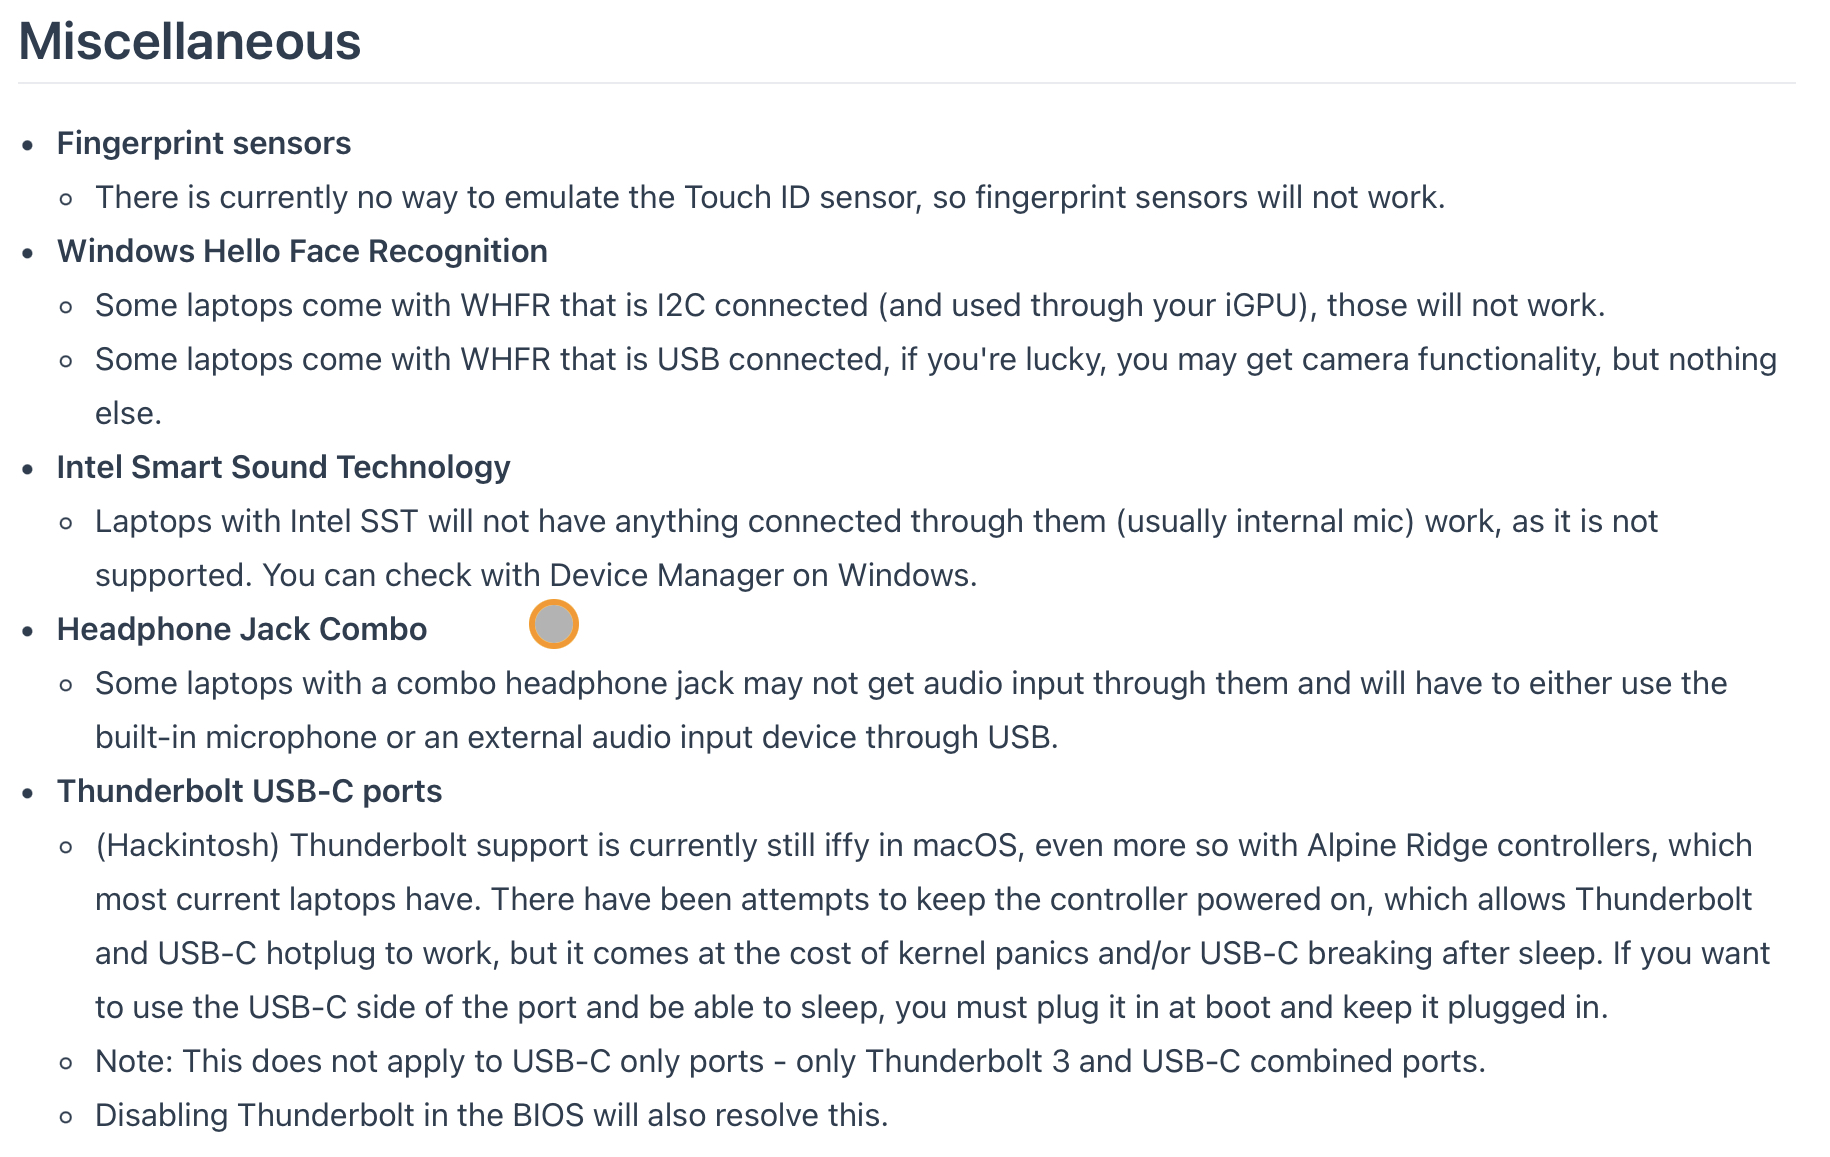
\includegraphics[width=0.8\textwidth]{fotos/PSP/Research/Native/Opendoe req misc.jpeg}
\break
\emph{Misc requirements}
\hfill\break
\hfill\break
Thunderbolt and biometrics do not work and Windows Hello are not compatible just yet.
\newpage
\subsection{Virtualization}
The best method and the possible future solution. Since that, you can fake the components with any server components and simulate everything without any issues. There are 2 best options One is BareMetal OS or Kernel-based Virtual Machine with PCI passthrough.

\hfill\break
\hfill\break
Let's start with KVM. The best-chosen KVM is QEMU.
\hfill\break

\includegraphics[width=0.8\textwidth]{fotos/PSP/Research/Virtualization/Qemu.jpeg}
\break
\emph{Logo of Qemu}
\hfill\break
\hfill\break
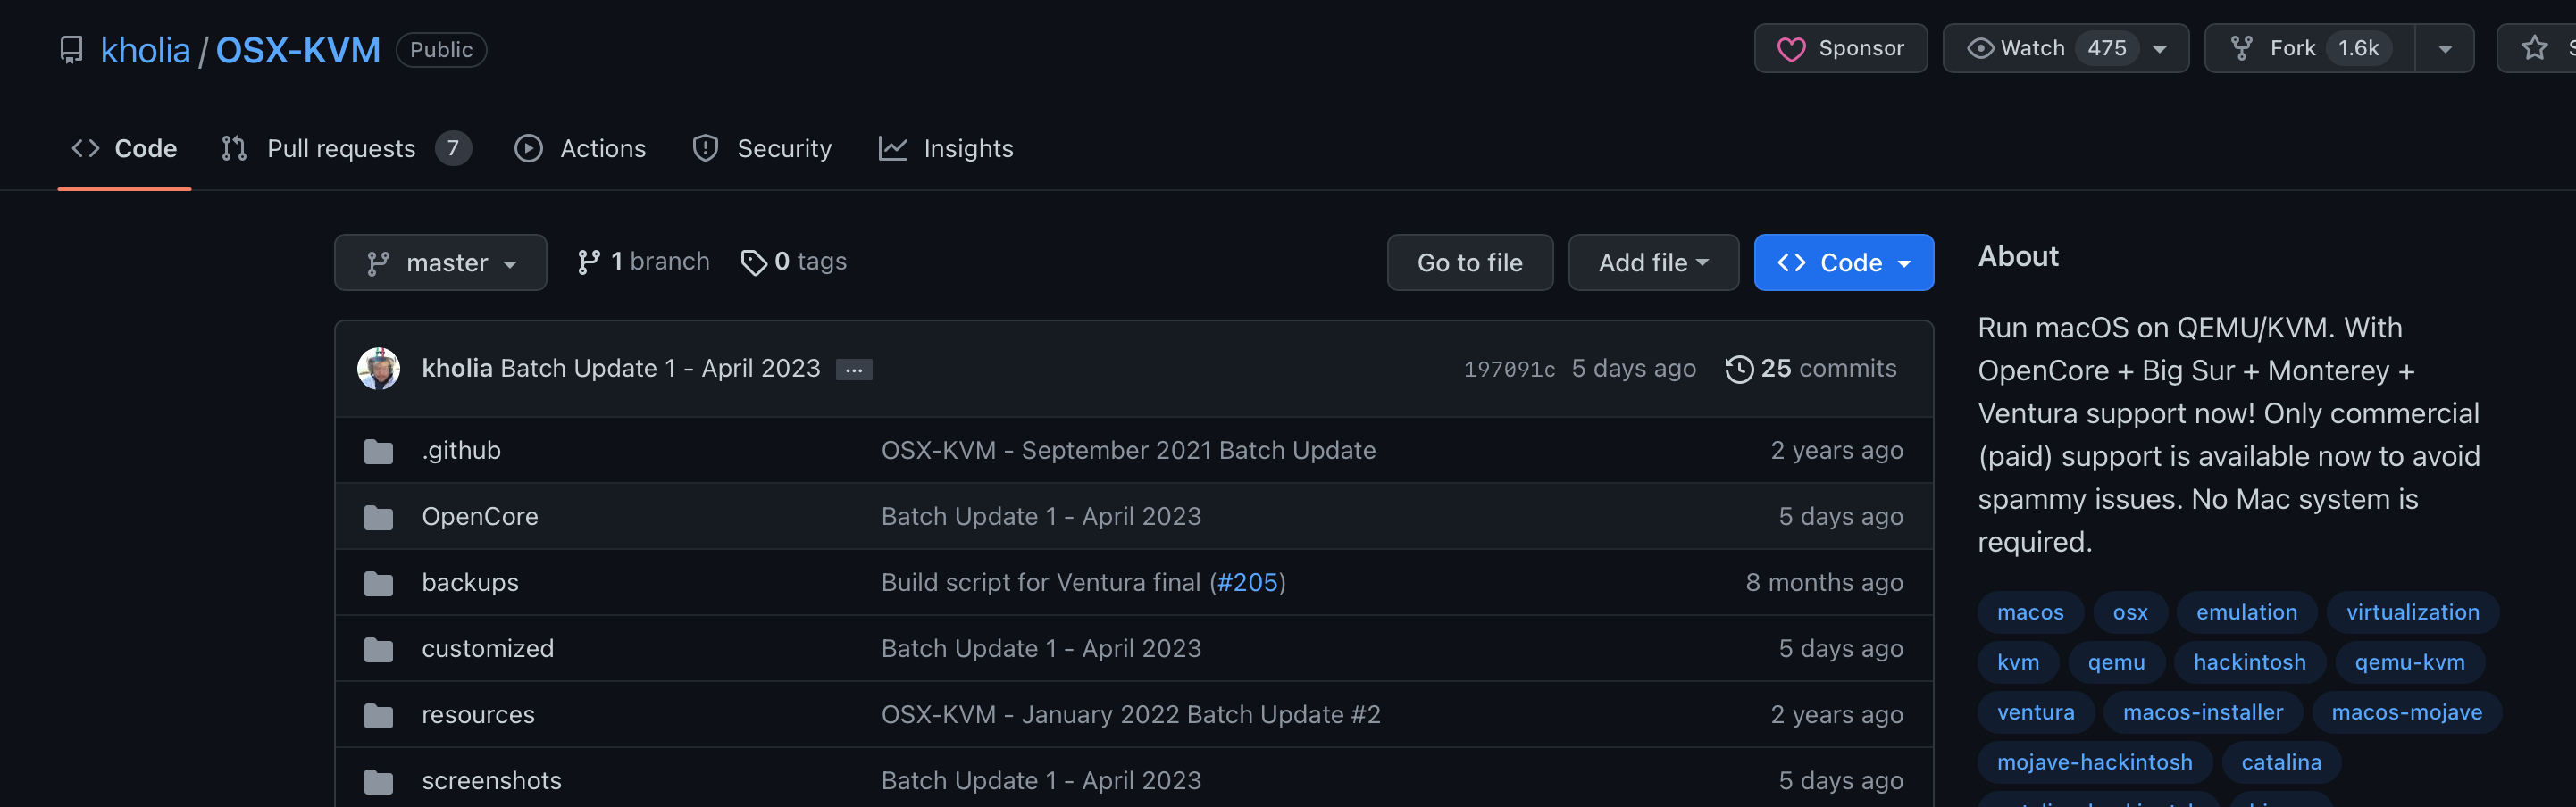
\includegraphics[width=0.9\textwidth]{fotos/PSP/Qemu/IMG_0865.jpeg}
\break
\emph{Github for KVM macOS}

\newpage
\subsection{Spoofing old hardware}
Spoofing old hardware means running old Mac devices which are no longer supported by Apple. The community were clever to find a way to spoof and modify macOS.
\hfill\break
\hfill\break
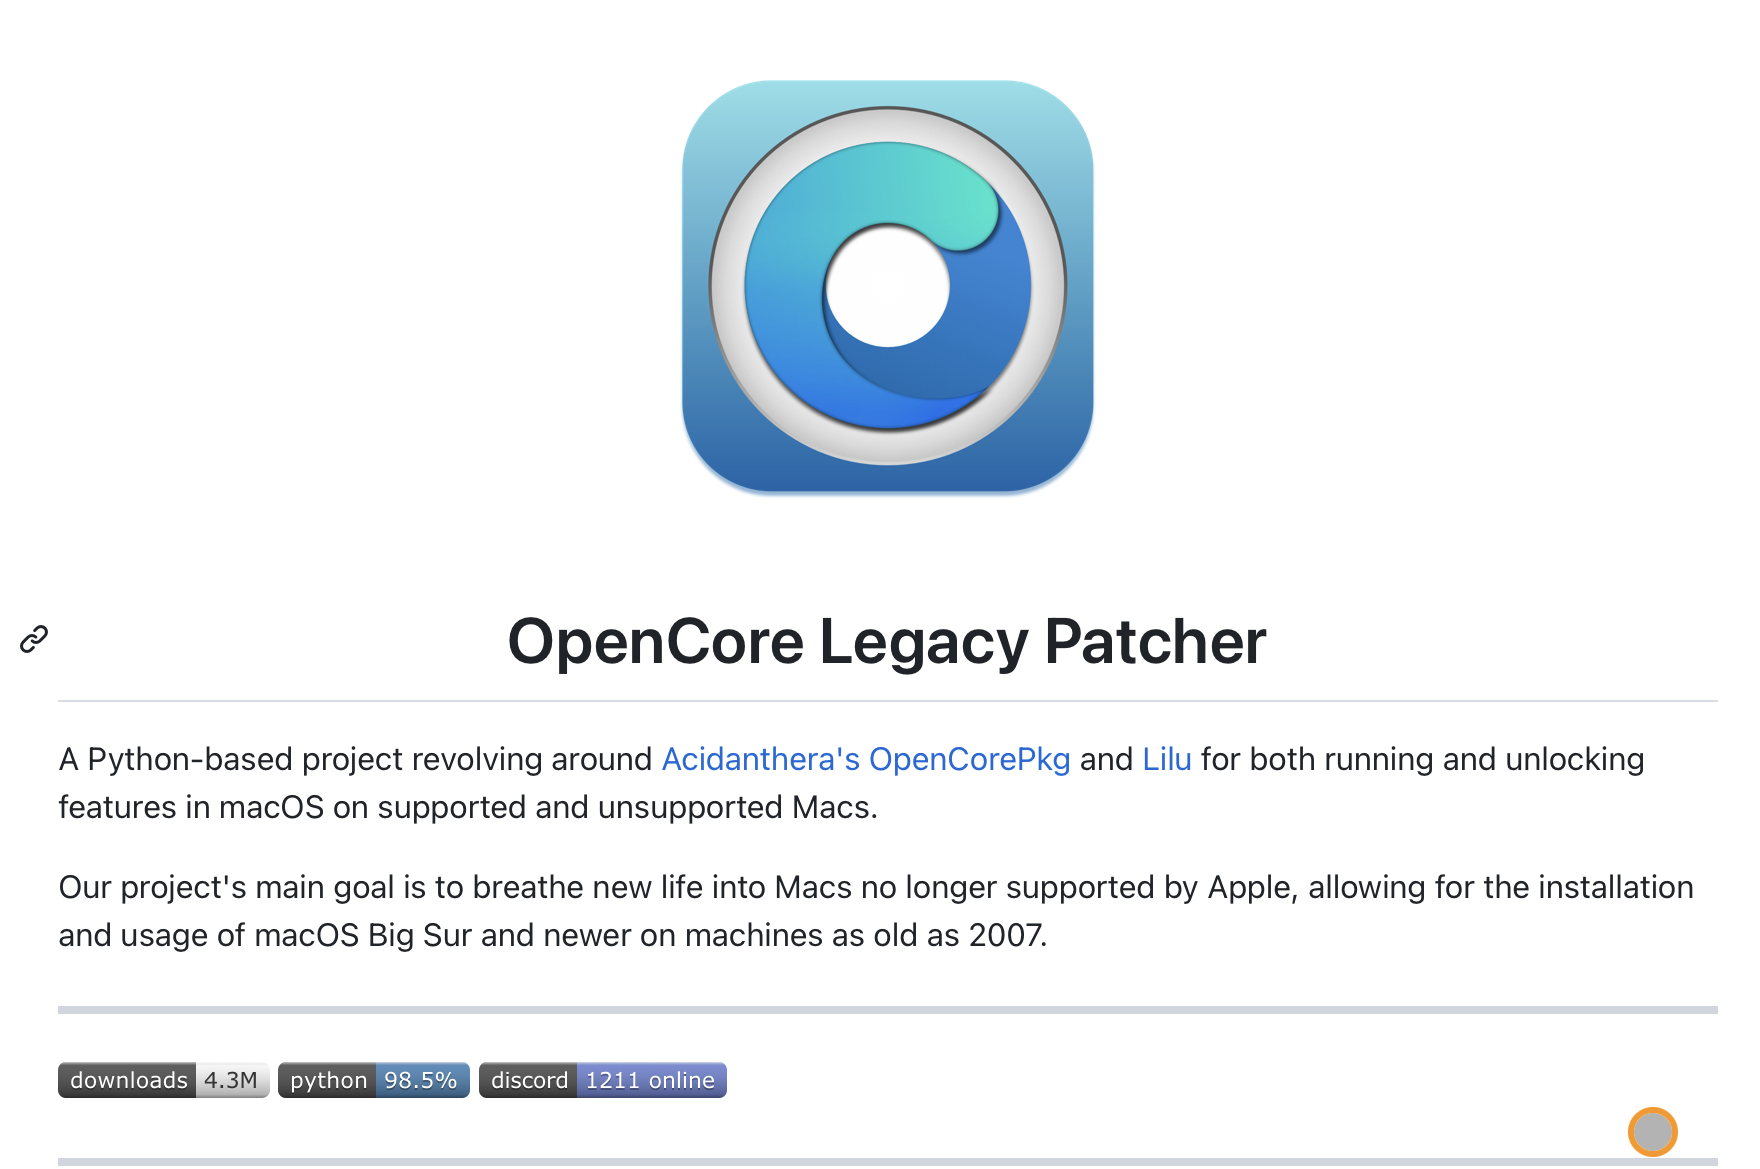
\includegraphics[width=0.8\textwidth]{fotos/PSP/Research/Lucy patcher/IMG_0807.jpeg}
\break
\emph{This tool helps old macs to run new macOS \url{https://github.com/dortania/OpenCore-Legacy-Patcher}}
\hfill\break
\hfill\break
This tool helps you update your old crusty Mac into the new and better macOS. Not only that it brings back old drivers like wifi and GPU drivers. Their GitHub page mentions their cool features like.
\begin{itemize}
    \item Support for macOS Big Sur, Monterey and Ventura
    \item Native Over the Air (OTA) System Updates
    \item Supports Penryn and newer Macs
    \item Full support for WPA Wi-Fi and Personal Hotspot on BCM943224 and newer wireless chipsets
    \item System Integrity Protection, FileVault 2, .im4m Secure Boot and Vaulting
    \item Recovery OS, Safe Mode and Single-user Mode booting on non-native OSes
    \item Unlocks features such as Sidecar and AirPlay to Mac even on native Macs
    \item Enables enhanced SATA and NVMe power management on non-Apple storage devices
    \item Zero firmware patching required (ie. APFS ROM patching)
    \item Graphics acceleration for both Metal and non-Metal GPUs
\end{itemize}
\newpage
\section{Legality}
\subsection{Software Licensing}
According to Apple End User License Agreement (EULA) mentions that macOS can only be installed on Apple hardware. This means what we are doing is breaking End User License with Apple which violates the licensing agreement.

\subsection{Intellectual Property Rights}
\textbf{According to Apple property rights}: Apple holds intellectual property rights over macOS, including its code, design, and user interface. Modifying or circumventing the operating system to run on non-Apple hardware can be seen as violating these intellectual property rights.

\subsection{What does this mean for the Hackintosh user}
Since this is breaking their Intellectual Property (IP) they have the full right to ban my Apple ID which I use and would not want to be banned. No one in modern times got banned(Only locked from Facetime and iMessage) because of it. Apple knows most people from the Hackintosh community eventually will buy a Mac device sooner or later.

\newpage
\section{Research questions}

\subsection{Main question}
What are the  motivations behind installing Hackintosh on a laptop or PC?

\subsection{Sub questions}
\begin{enumerate}
    \item What are the advantages and disadvantages of running macOS on non Apple hardware through Hackintosh?
    \item How does the performance of a Hackintosh system running Swift and Xcode compare to that of a Mac for compiling, debugging, and running iOS/macOS apps?
    \item How is the future of Hackintosh?
\end{enumerate}
\section{Materials}
To create a test environment, I need to have the materials to run this test if it is true.
\begin{enumerate}[label=(\roman*)]
    \item MSI GF63 8rc
    \item A legal copy of macOS
    \item a 16gb USB stick (USB 2.0 preferred)
\end{enumerate}
\subsection{Tools}
\begin{enumerate}
    \item Propertree 
    \item Bunch of KEXT files
    \item SSDT compilers
    \item Virtualbox/NAT
\end{enumerate}

\section{Results}


\subsection{Research}

Before I started to do hackintosh I went on Youtube to find some videos for how to install Hackintosh on your desktop/laptop.
\hfill\break
\hfill\break
After following the youtube video i went to the site called Dortania guide.
\hfill\break
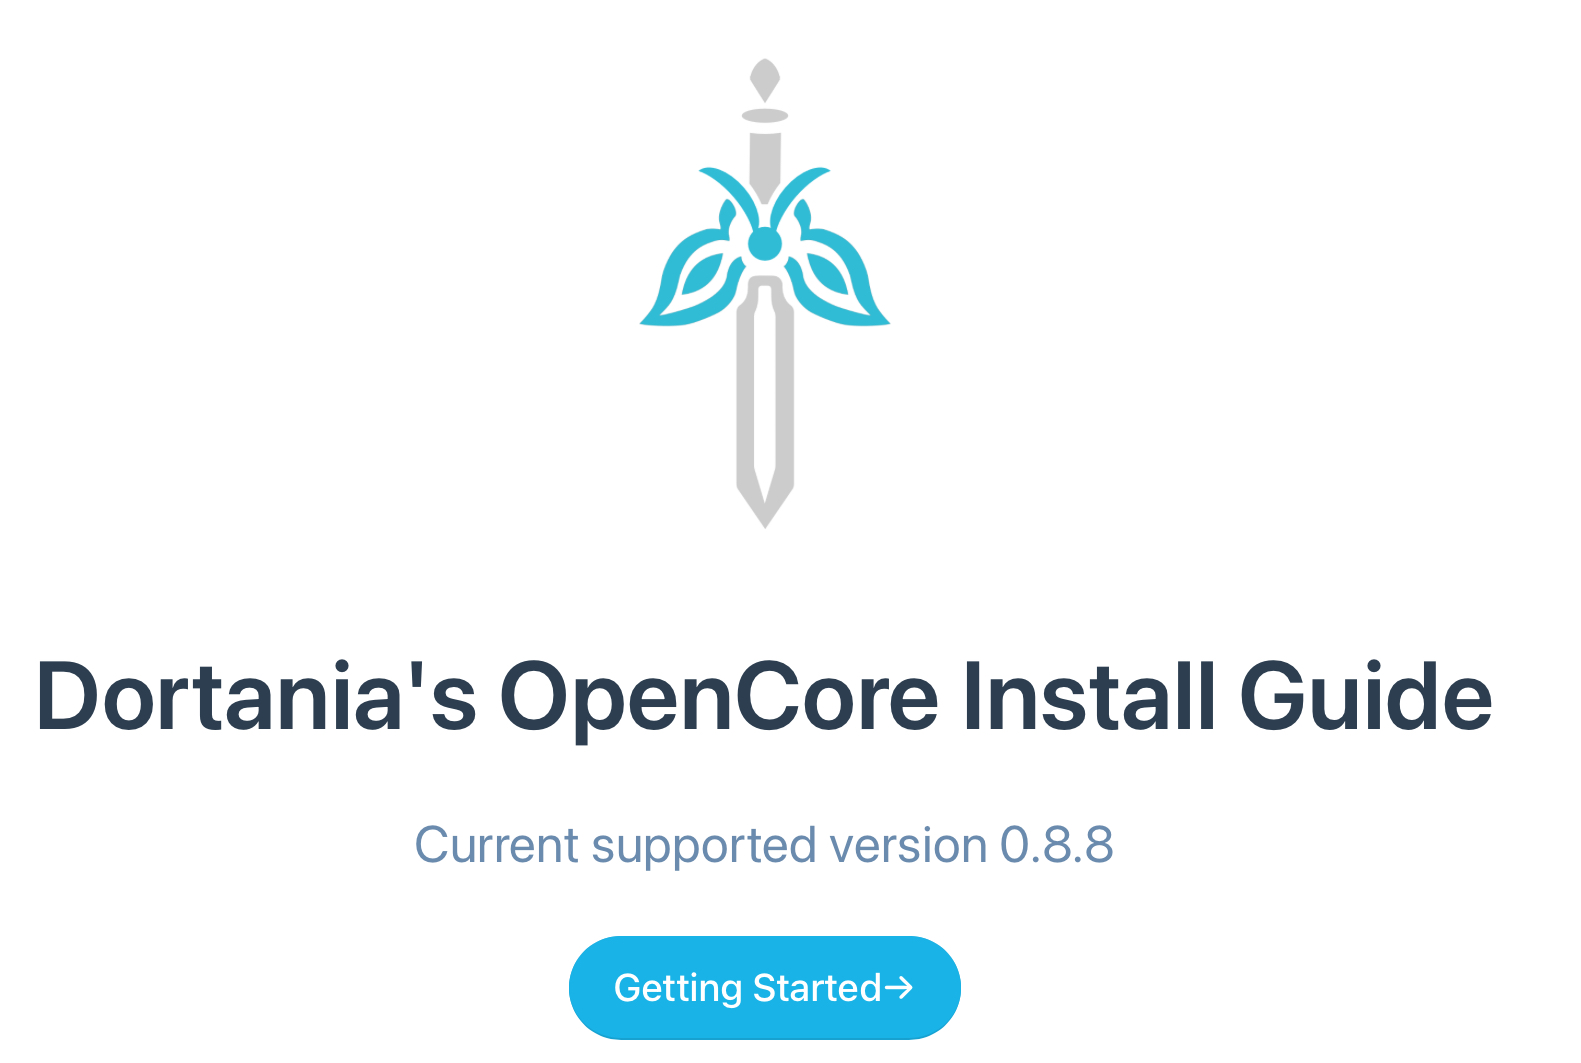
\includegraphics[width=0.8\textwidth]{fotos/PSP/Research header/Dortania opencore.jpeg}
\break
\emph{Page of Dortania Guide}
\hfill\break
\hfill\break
After finding some LEGAL Apple macOS Montery basefile.dmg we can finally start imaging our usb stick.
\hfill\break
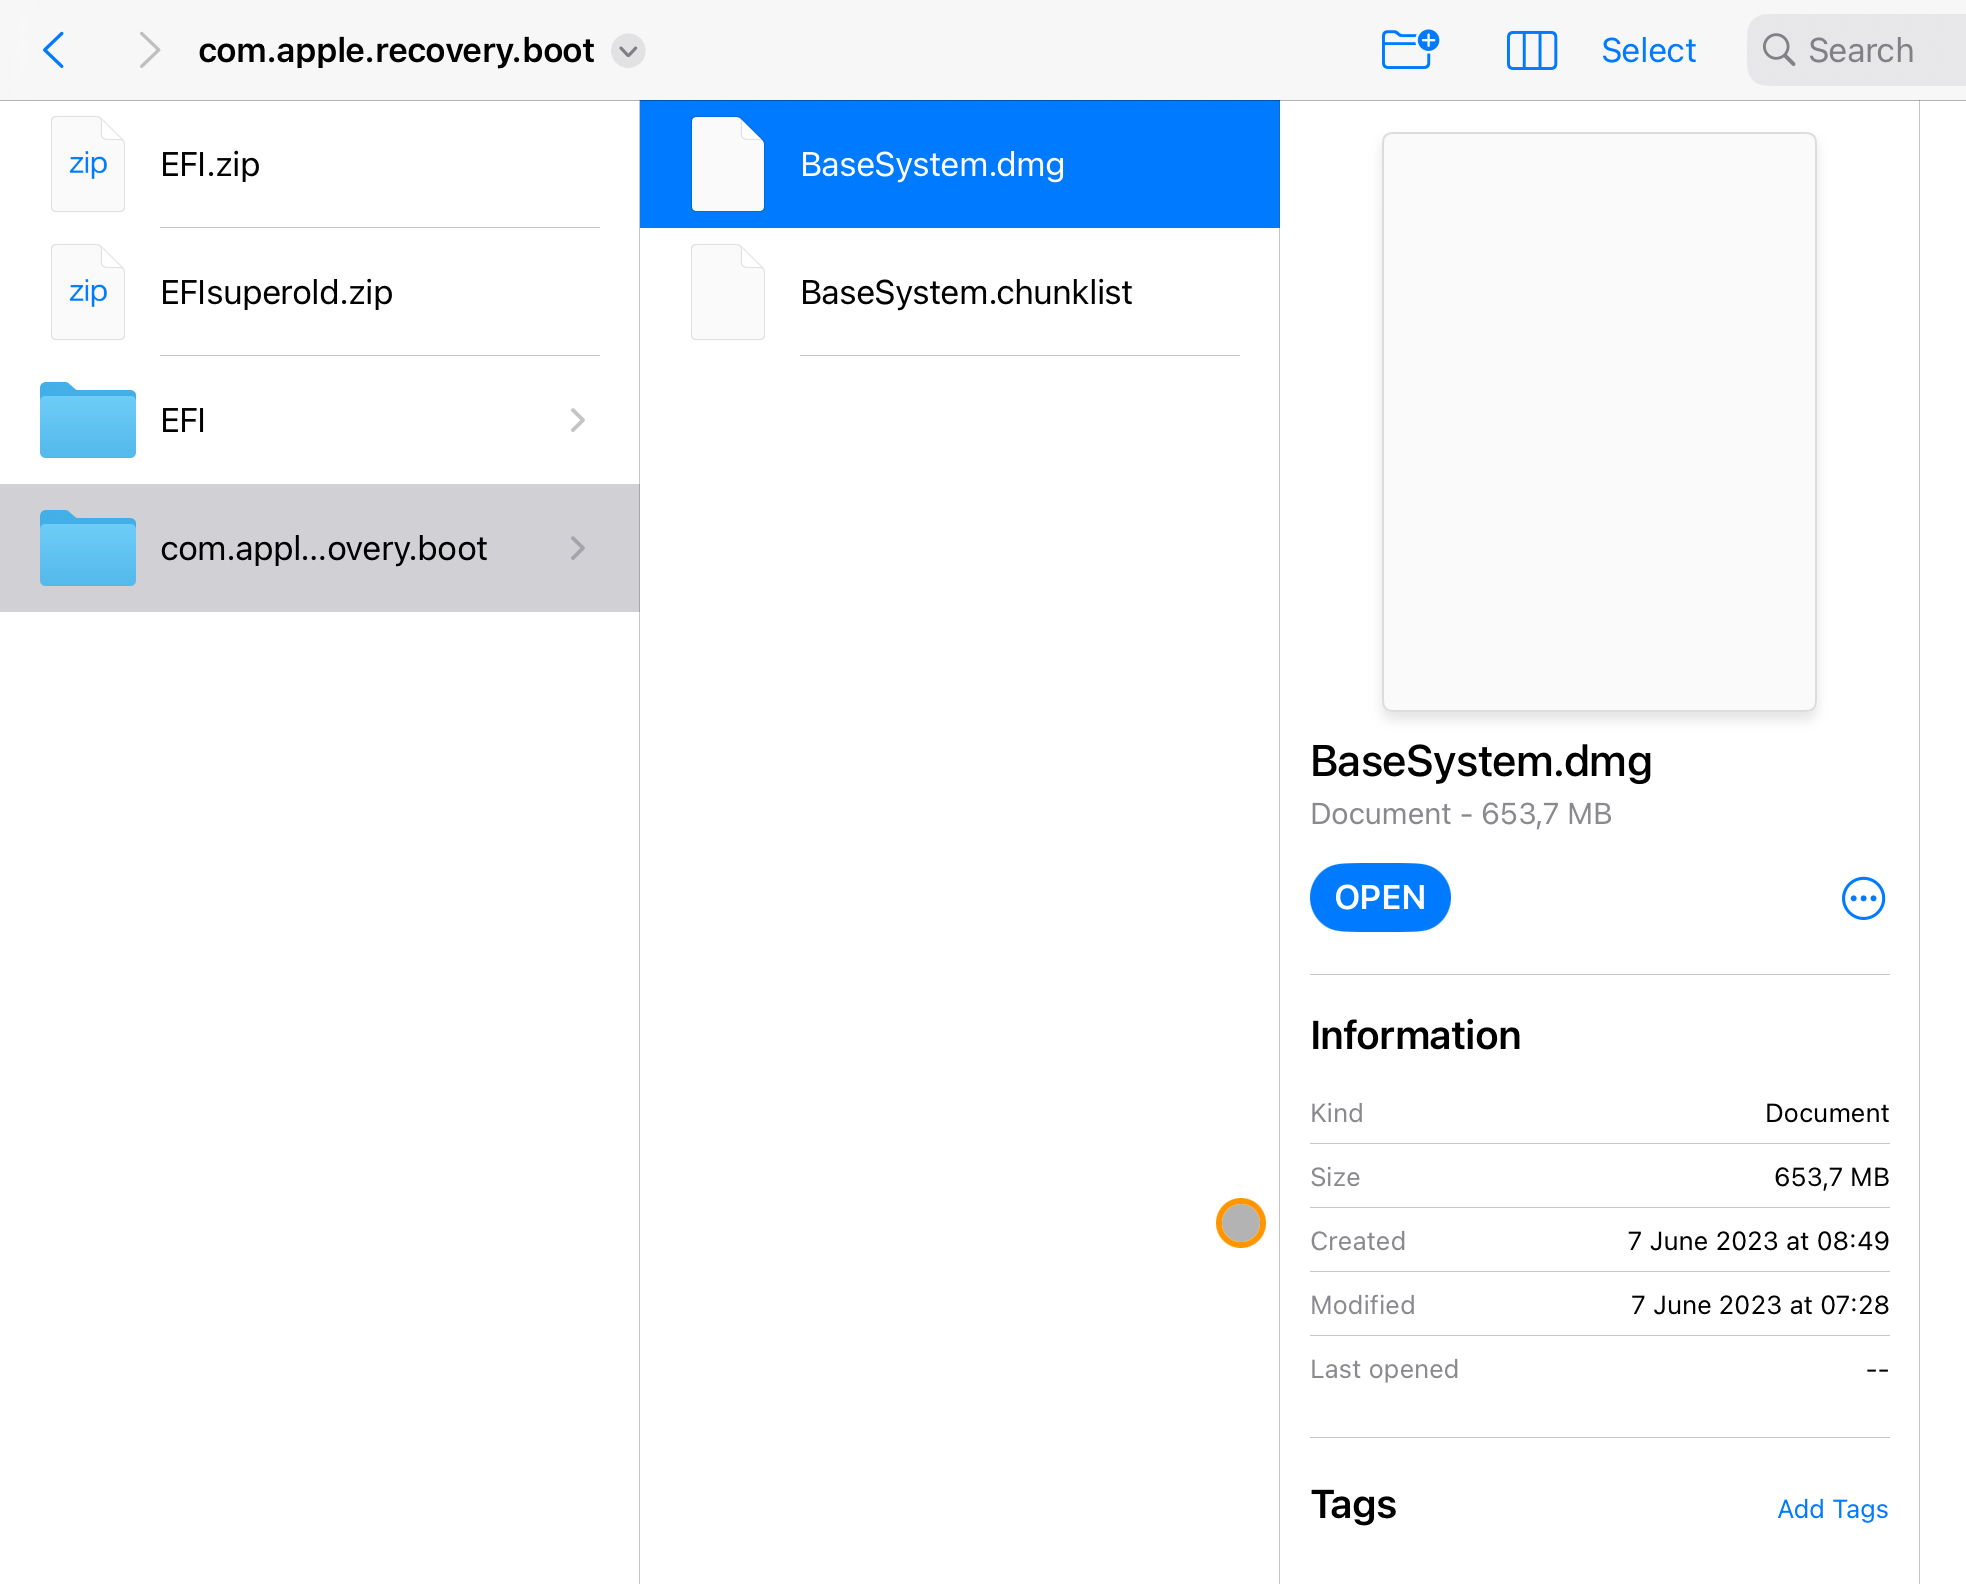
\includegraphics[width=0.8\textwidth]{fotos/PSP/Research header/Montereydmg.jpeg}
\break
\emph{Original copy of Montery downloaded from Apple servers.}
\hfill\break
\hfill\break
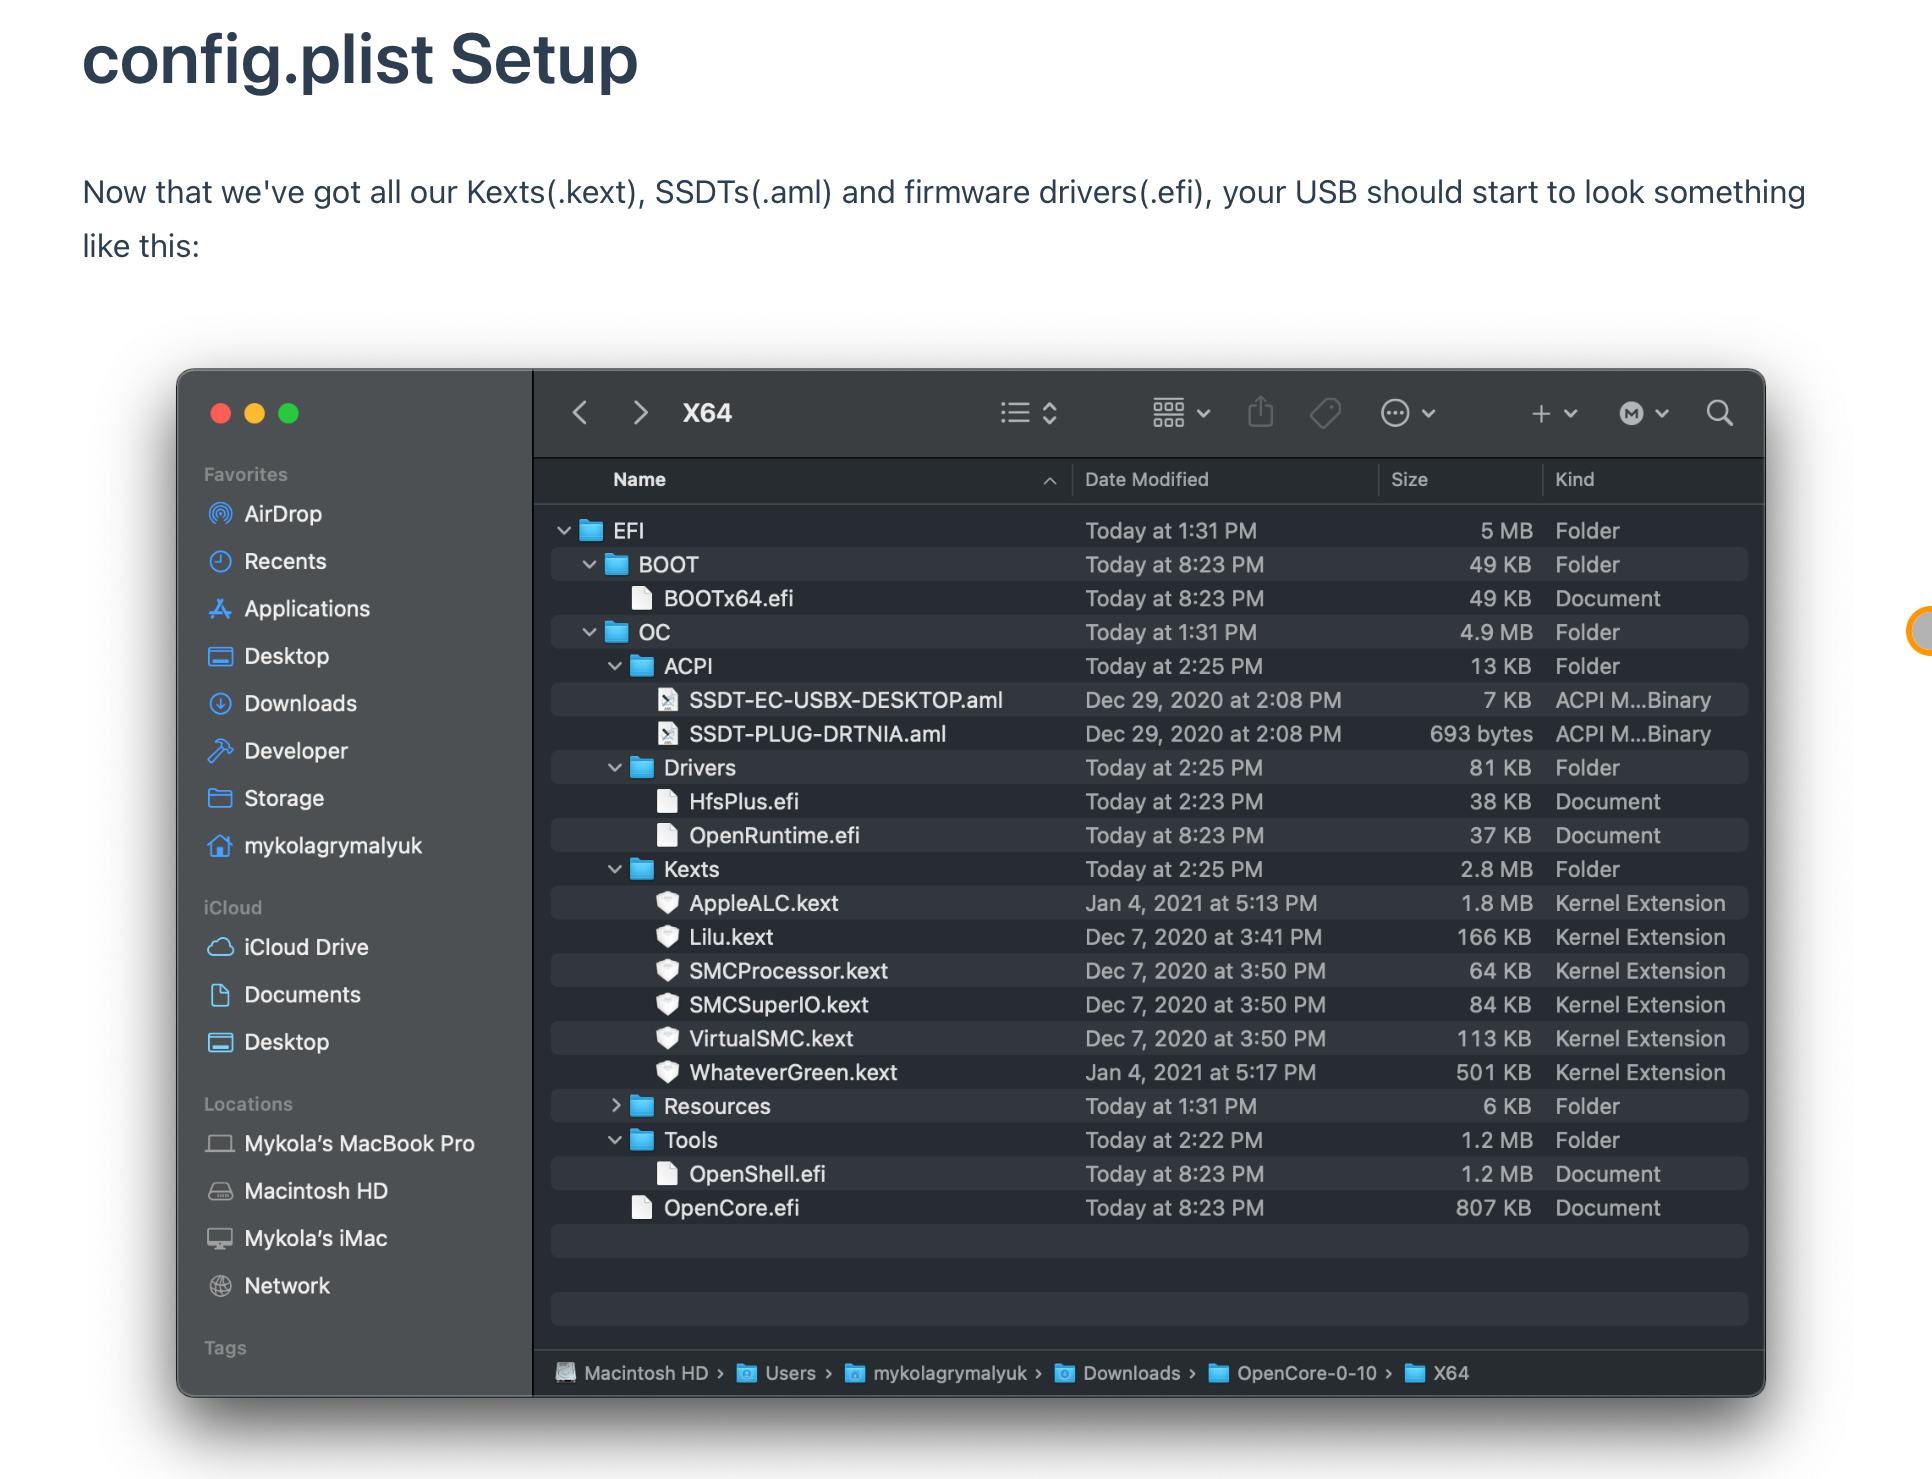
\includegraphics[width=0.8\textwidth]{fotos/PSP/Research header/Sampleconfigplist.jpeg}
\break
\emph{Now we download the config file so we can configure it.}
\hfill\break
\hfill\break
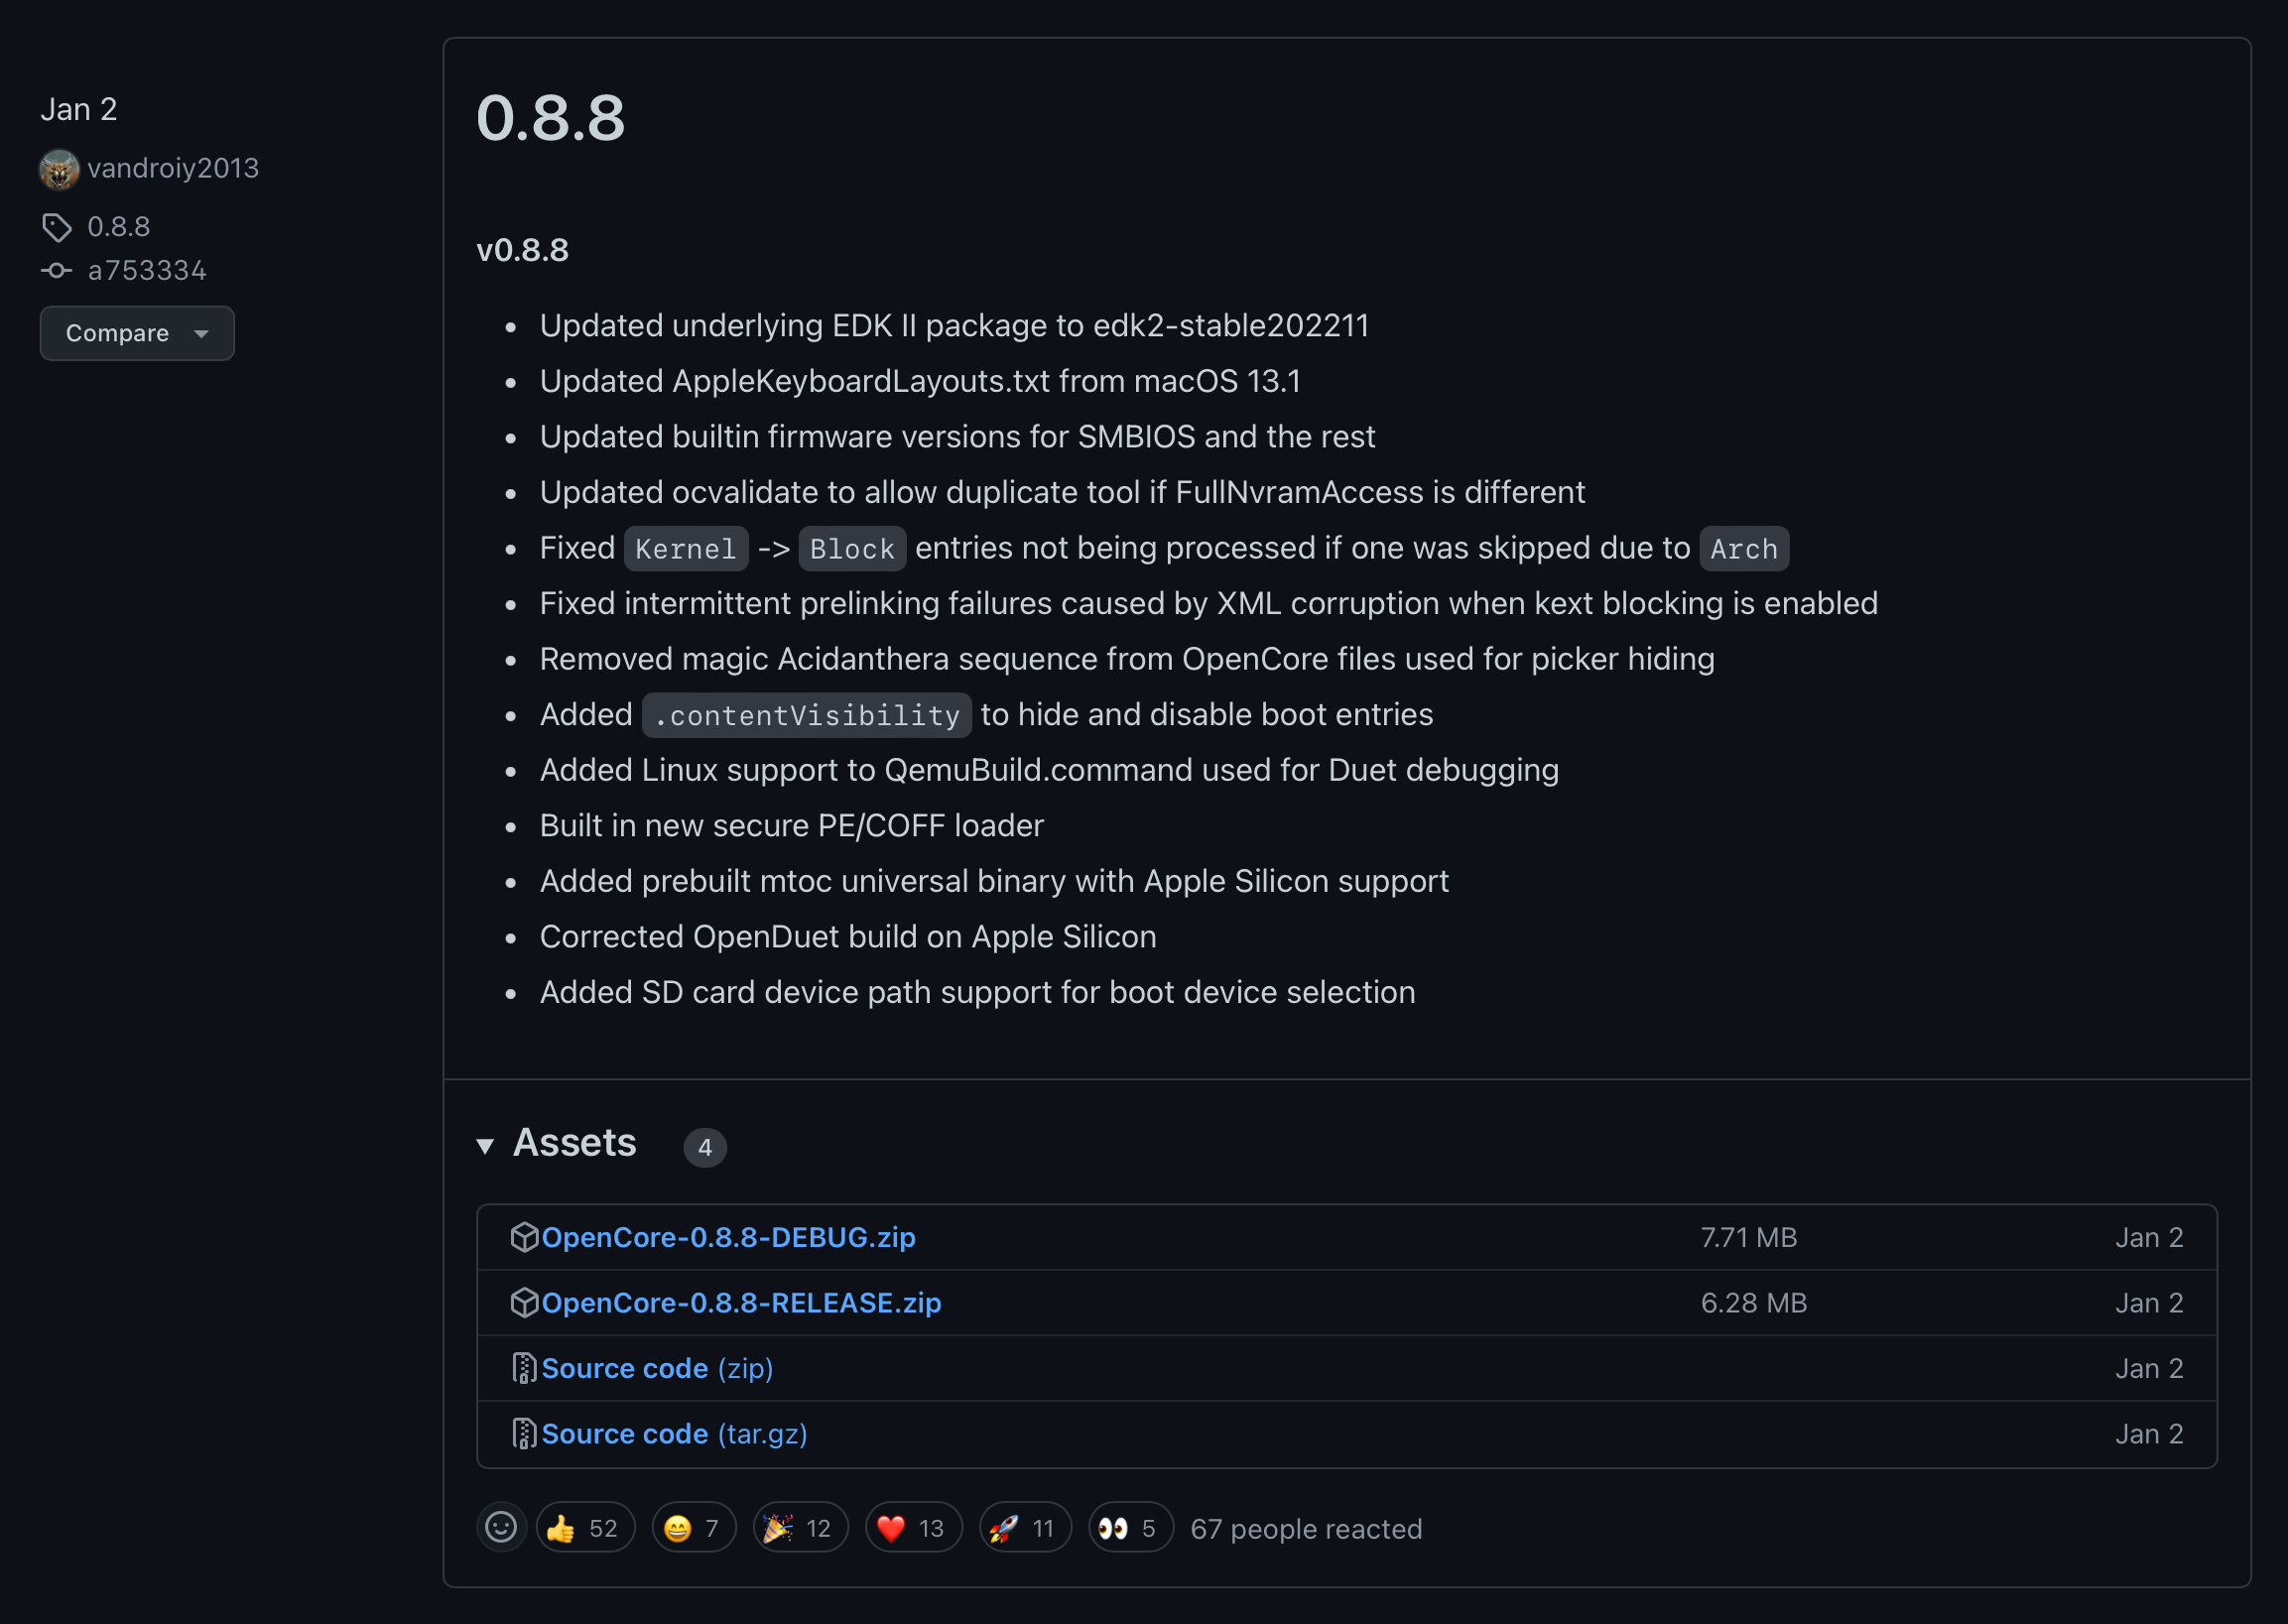
\includegraphics[width=0.8\textwidth]{fotos/PSP/Research header/Downloadopencore.jpeg}
\break
\emph{Downloading OpenCore config}
\hfill\break
\hfill\break
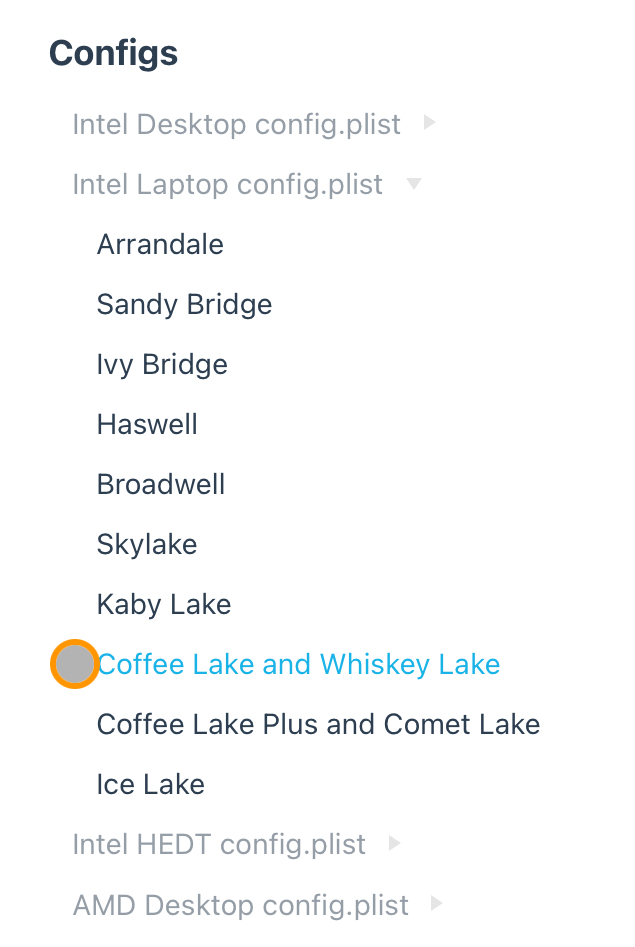
\includegraphics[width=0.8\textwidth]{fotos/PSP/Research header/Laptopconfig.jpeg}
\break
\emph{Continue as my laptop is Coffee Lake}
\hfill\break
\hfill\break
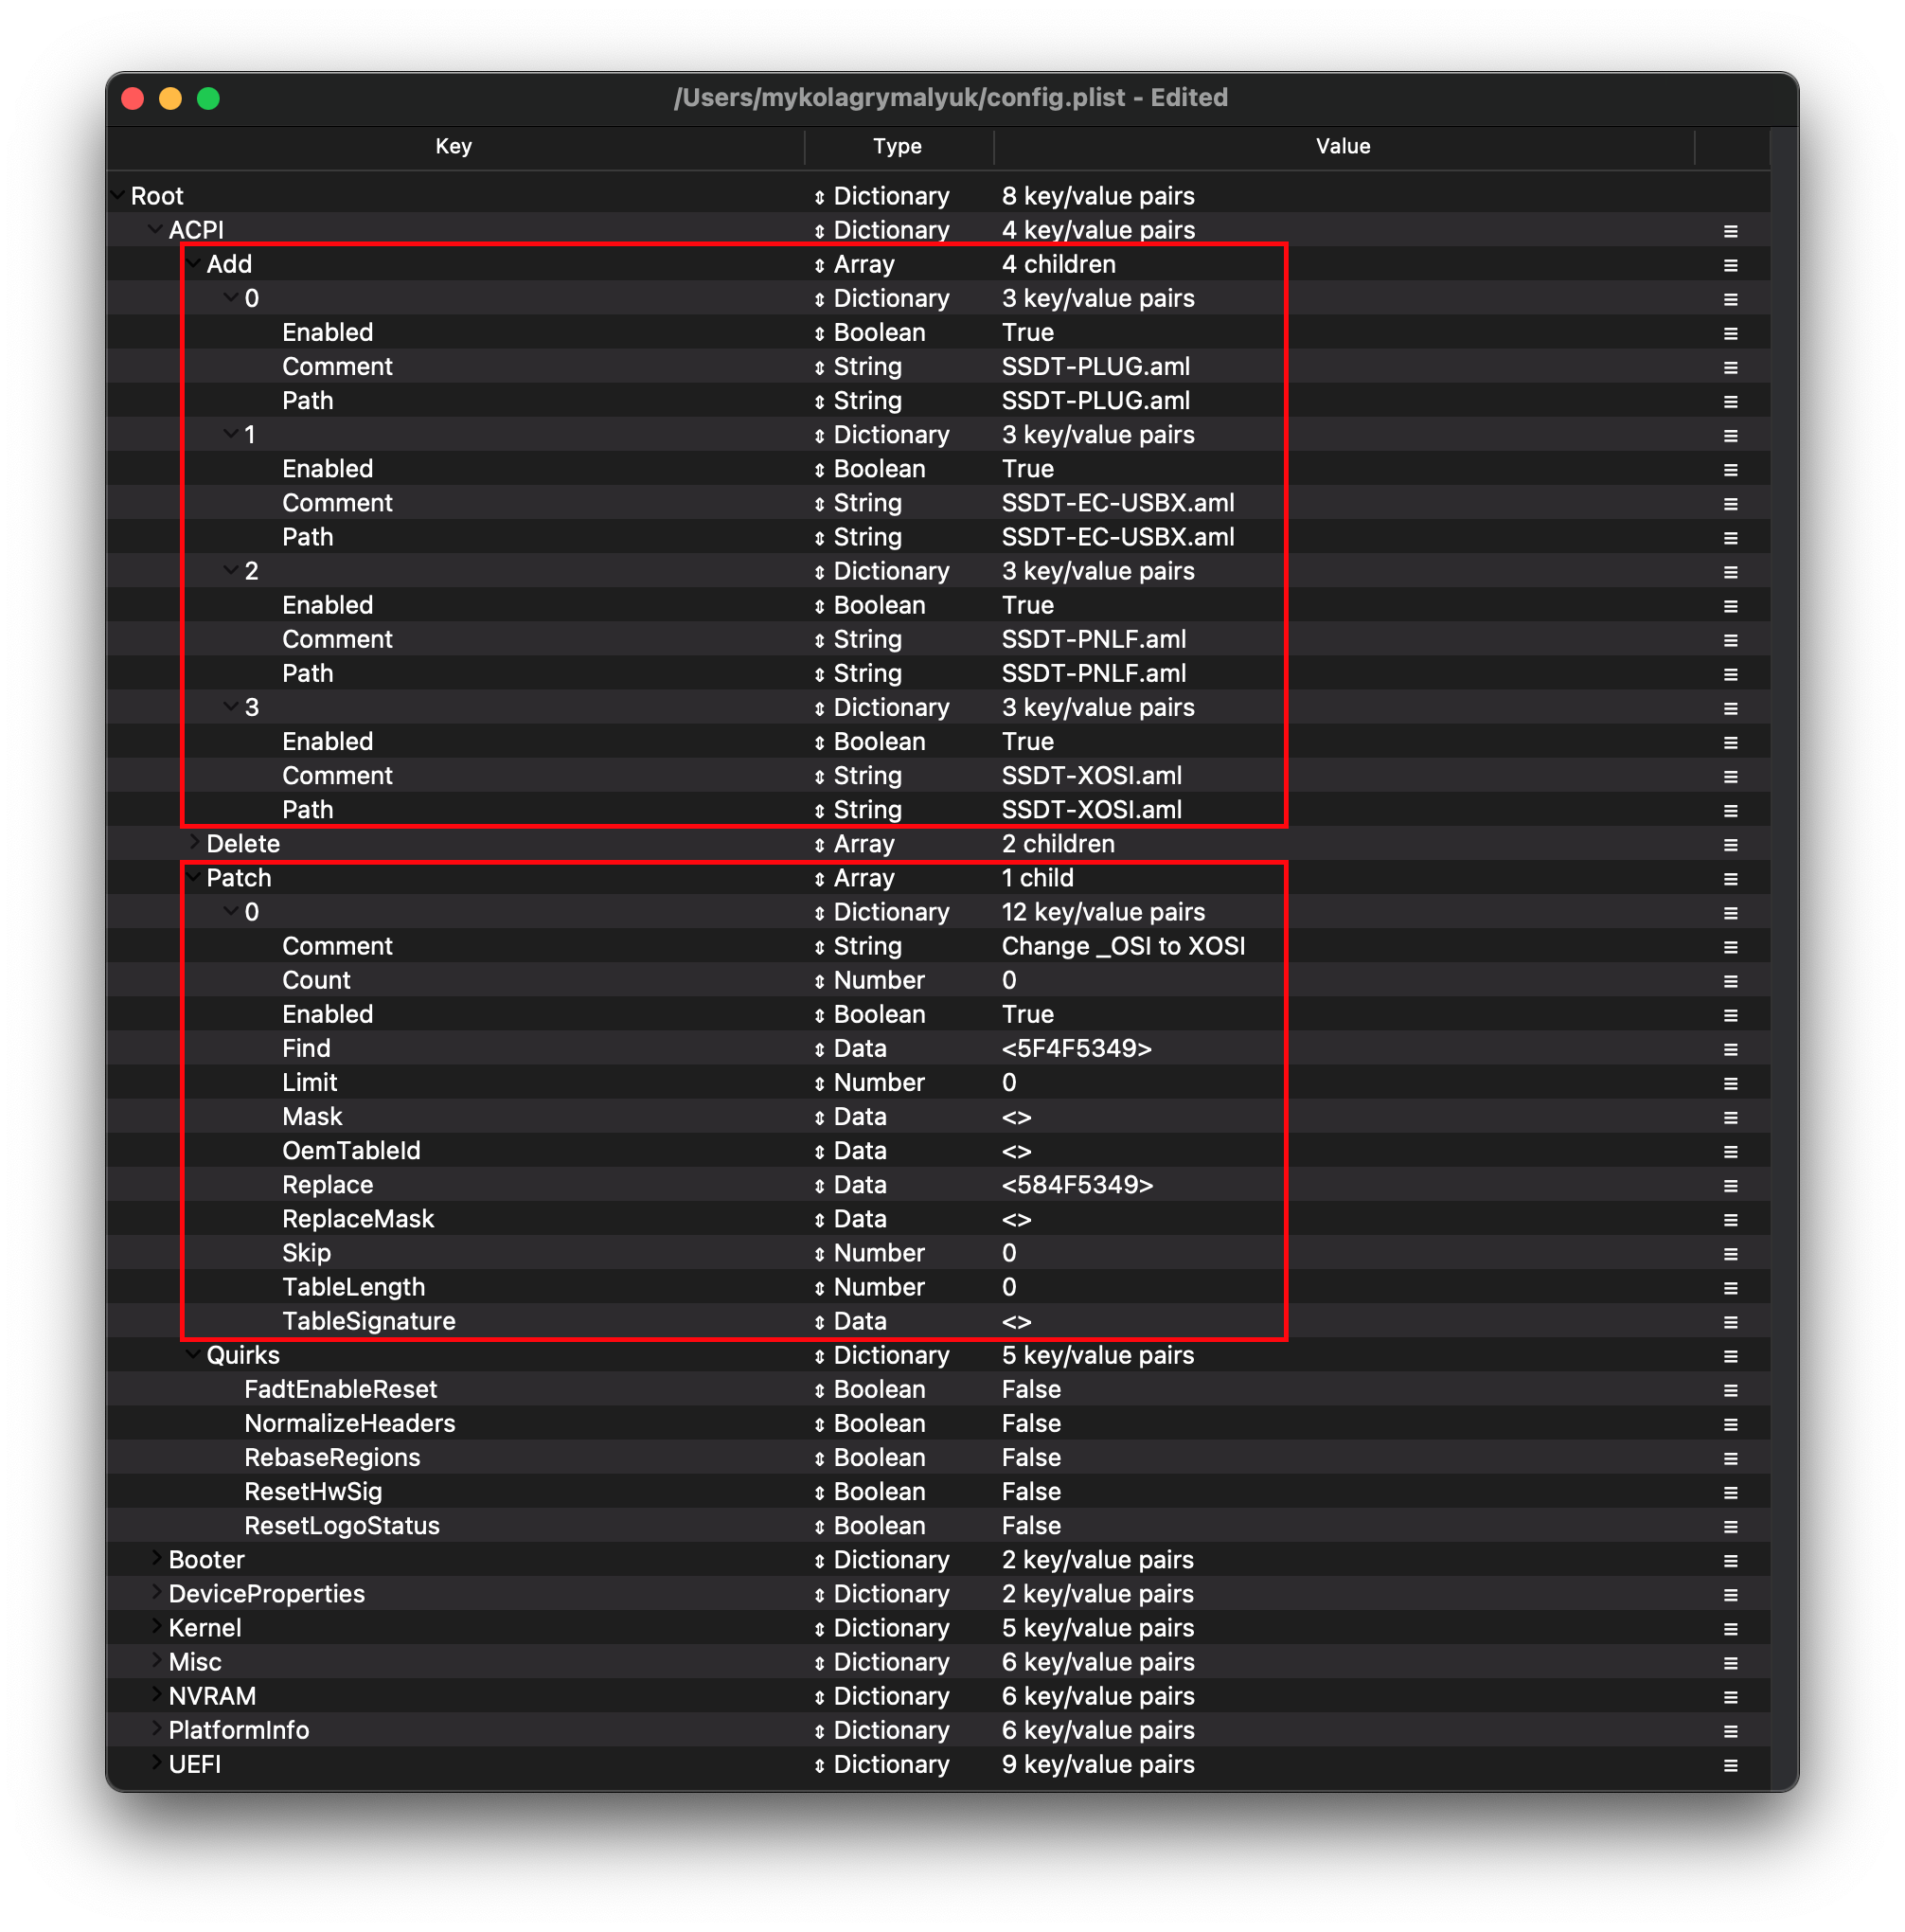
\includegraphics[width=0.8\textwidth]{fotos/PSP/Propertree/Acpi.png}
\break
\emph{Setting up ACPI in the config}
\hfill\break
\hfill\break
Since it's a preview from the document, we are going to put our own DSDT in Add tab so that the operating system gets a set of instructions for our CPU and Motherboard.
\hfill\break
\hfill\break
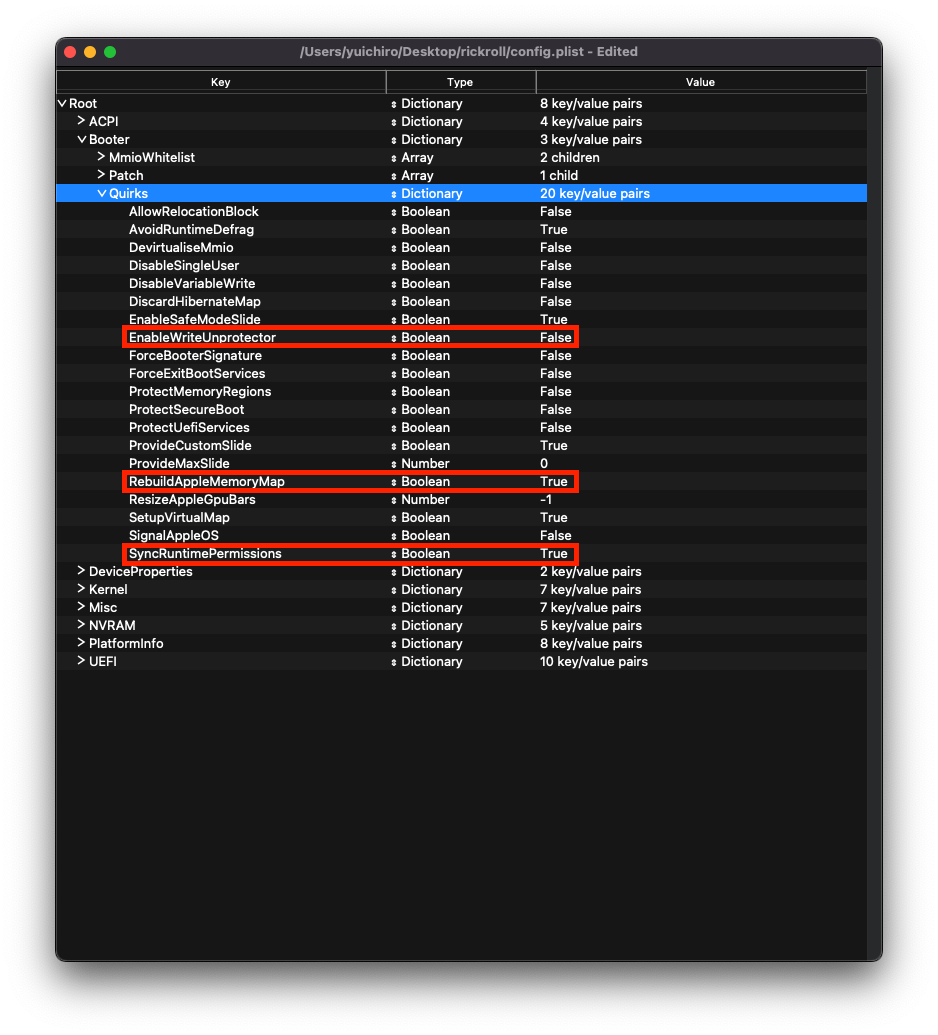
\includegraphics[width=0.8\textwidth]{fotos/PSP/Propertree/Booter.png}
\break
\emph{Configuring the booter}
\hfill\break
\hfill\break
Here we disable some settings like WriteUnprotector, RebuildAppleMemoryMap and SyncRuntimePermissions.
\begin{itemize}
    \item WriteUnprotector
    \break
    It is recommended if you want to run on newer mac versions
    \item RebuildAppleMemoryMap
    \break
    Generates Memory Map compatible with macOS
    \item SyncRuntimePermissions
    \break
    Fixes alignment with MAT tables
\end{itemize}
\hfill\break
\hfill\break
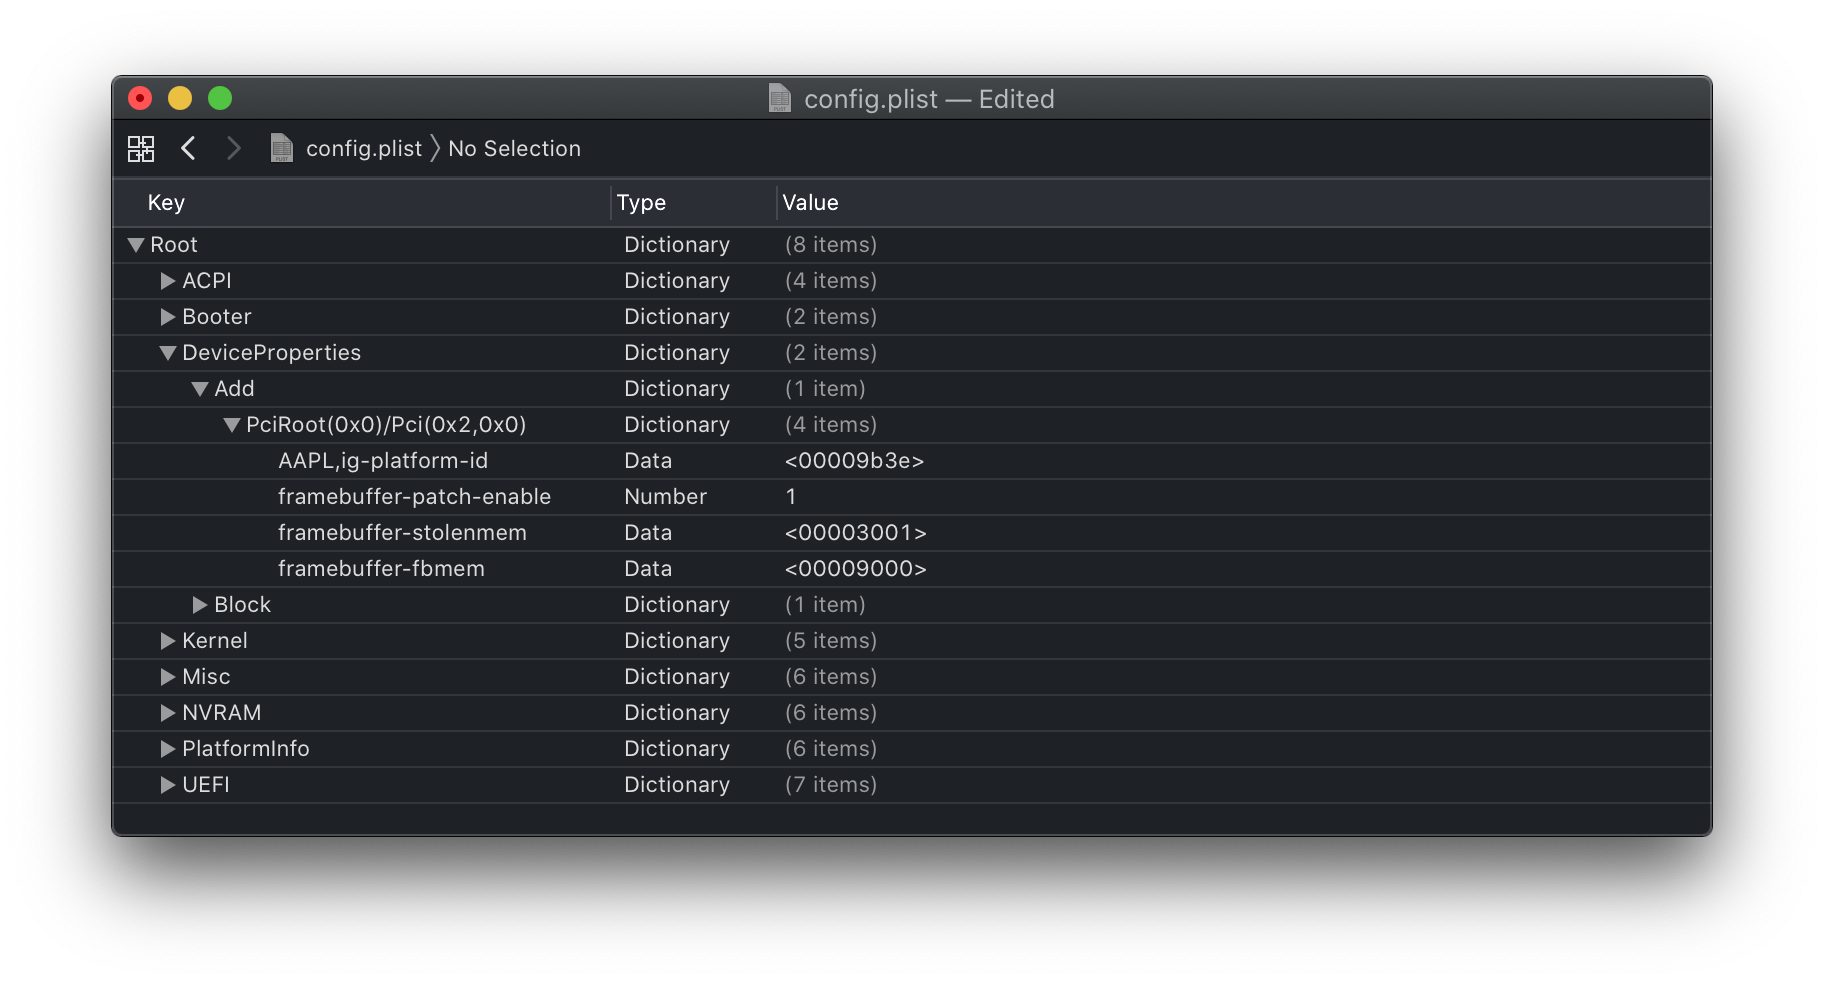
\includegraphics[width=0.8\textwidth]{fotos/PSP/Propertree/Deviceproperties.png}
\break
\emph{Compiling GPU in Device Properties}
\hfill\break
\hfill\break
Here we need to find our Intel UHD 630 Device ID and find the stolen memory values and the rest of the commands like "enablemetal" (Metal 3) and "enable-hdmi20" (enable hdmi) are optional.
\hfill\break
\hfill\break
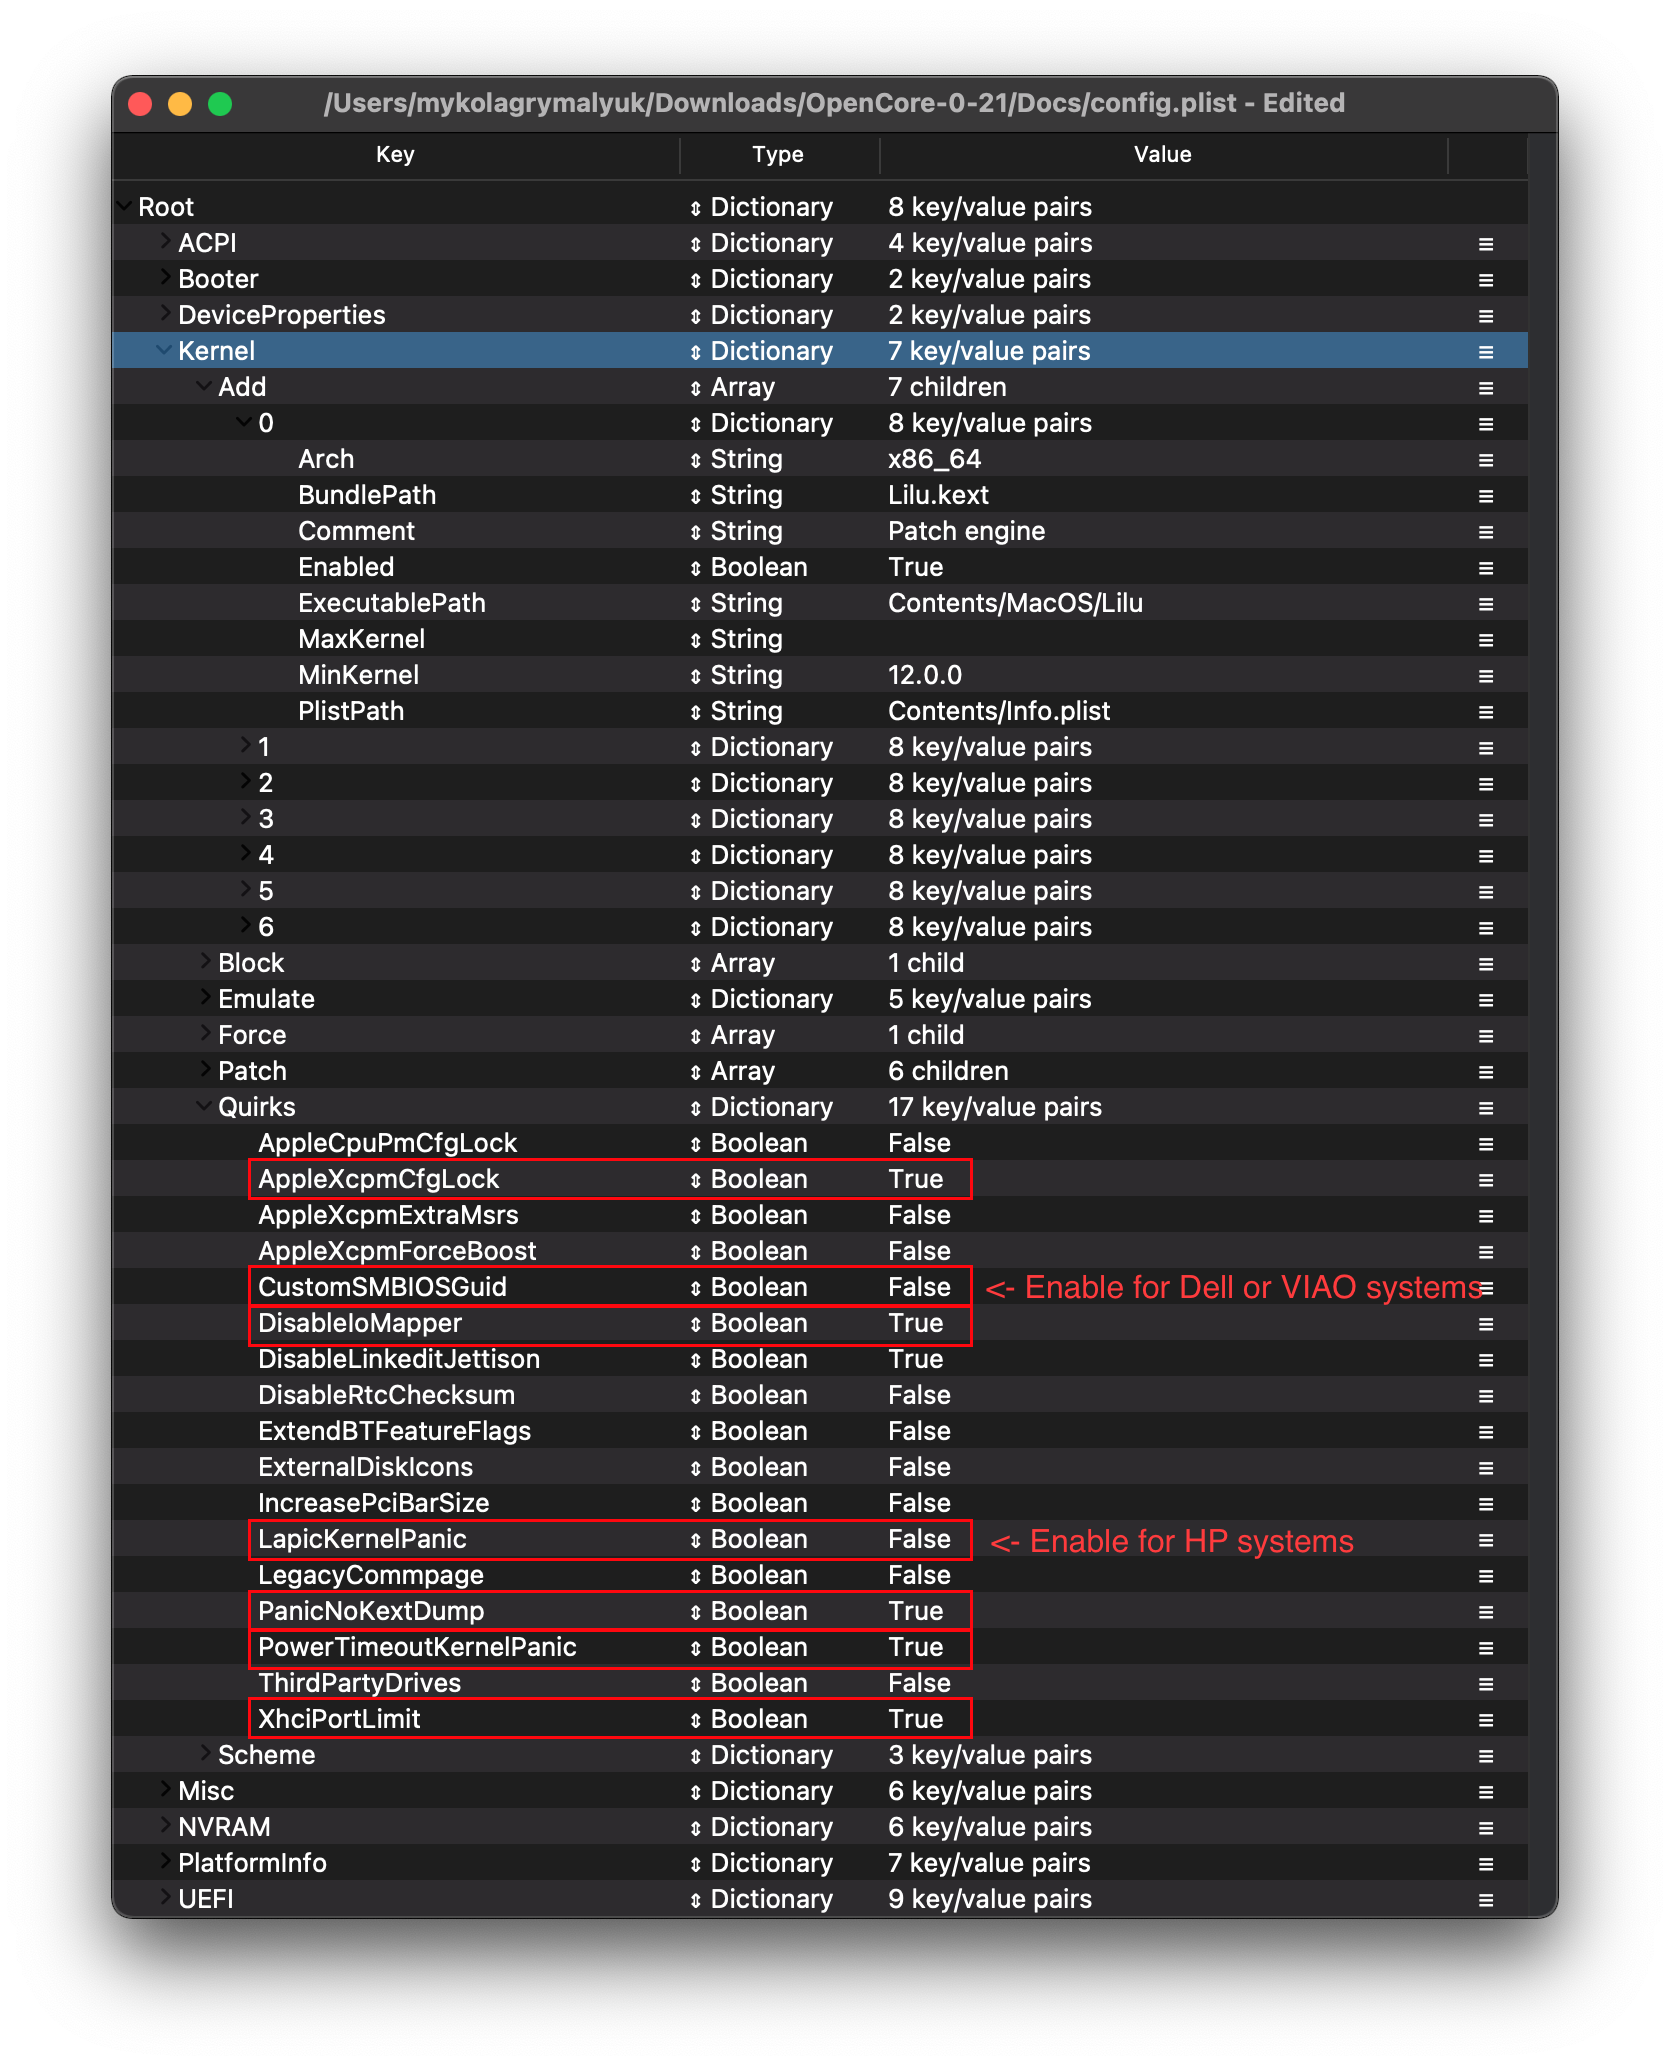
\includegraphics[width=0.8\textwidth]{fotos/PSP/Propertree/Kernel.png}
\break
\emph{Configuring the kernel}
\hfill\break
\hfill\break
Here we change some settings like AppleXcpmCfgLockm, DisableioMapper, PanicnoKextDump and PowerTimeoutKernelPanic. Since we run Monterey where you need to map your own USB so XhciPortLimit would not work in Monterey
\hfill\break
\hfill\break
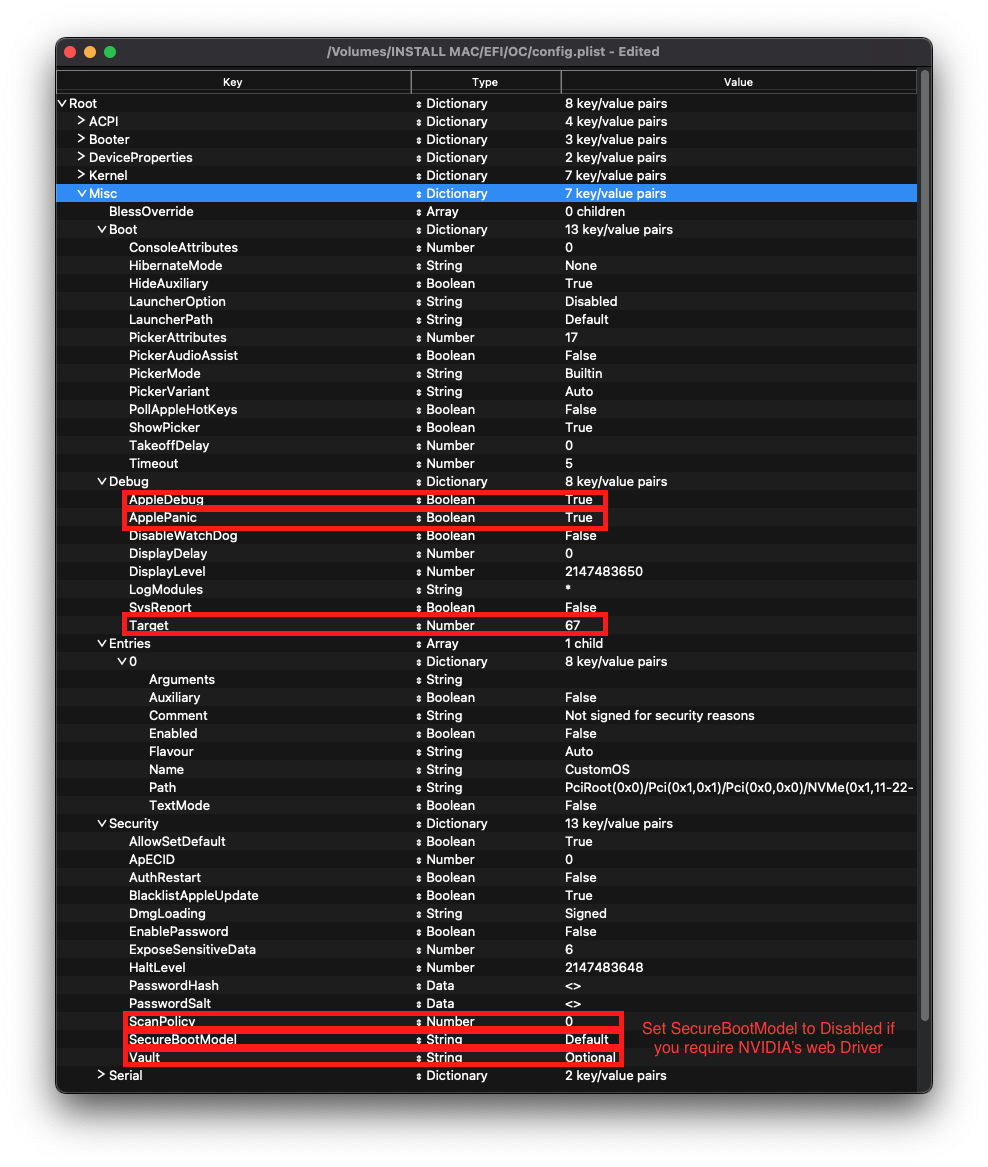
\includegraphics[width=0.8\textwidth]{fotos/PSP/Propertree/Misc.png}
\break
\emph{Configuring misc}
\hfill\break
\hfill\break
Here we configured some settings for our DMG file and if you want you can enable TPM here but for now we want to run before we make some changes.
\hfill\break
\hfill\break
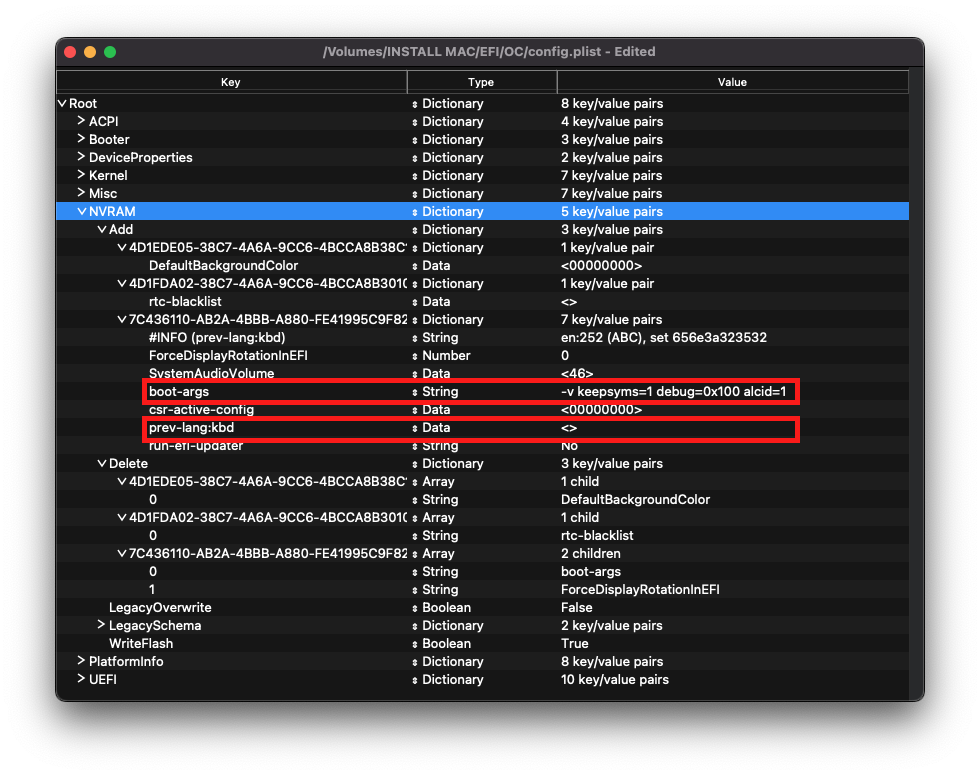
\includegraphics[width=0.8\textwidth]{fotos/PSP/Propertree/Nvram.png}
\break
\emph{Configuring NVRAM}
\hfill\break
\hfill\break
This is an important step for us since we have an unsupported Dedicated GPU and we need to disable it.
\hfill\break
\hfill\break
Here is my boot-args: -v -igfxvesa alcid=5 watchdog=0
\begin{itemize}
    \item -V
    \break
    Stands for Verbose.
    \item -igfxvesa
    \break
    It forces to run on Intel UHD graphics.
    \item alcid=5
    \break
    Apple Audio ID number 5 comes close to my audio card.
    \item Watchdog=0
    \break
    Disable Security and checksums from Apple server.
\end{itemize}

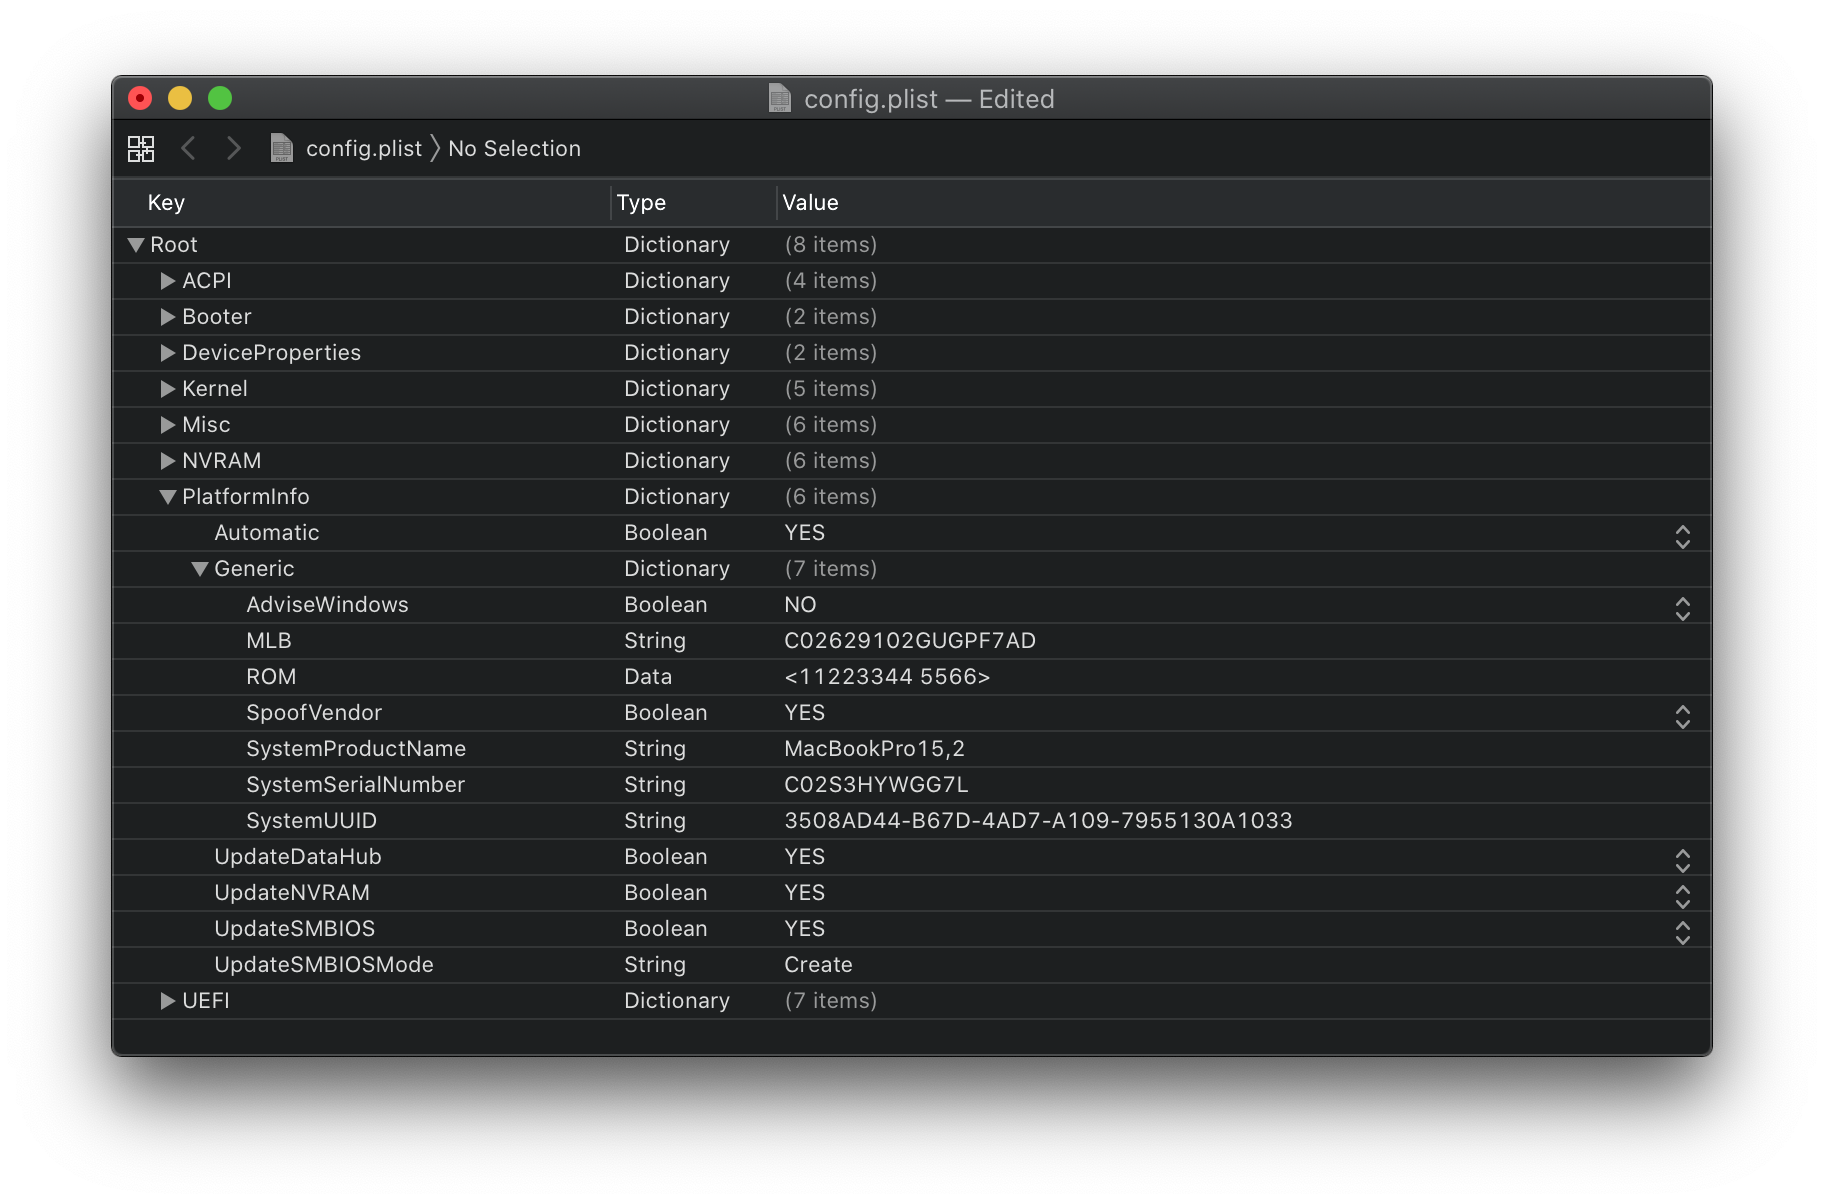
\includegraphics[width=0.8\textwidth]{fotos/PSP/Propertree/Platform info .png}
\break
\emph{Configuring Platforminfo}
\hfill\break
\hfill\break
Here we generate a fake ID and a fake platform. My system product is going to be MacBookPro15,1 which does not need Apple T2 security. and my serials will be randomized.
\hfill\break
\hfill\break
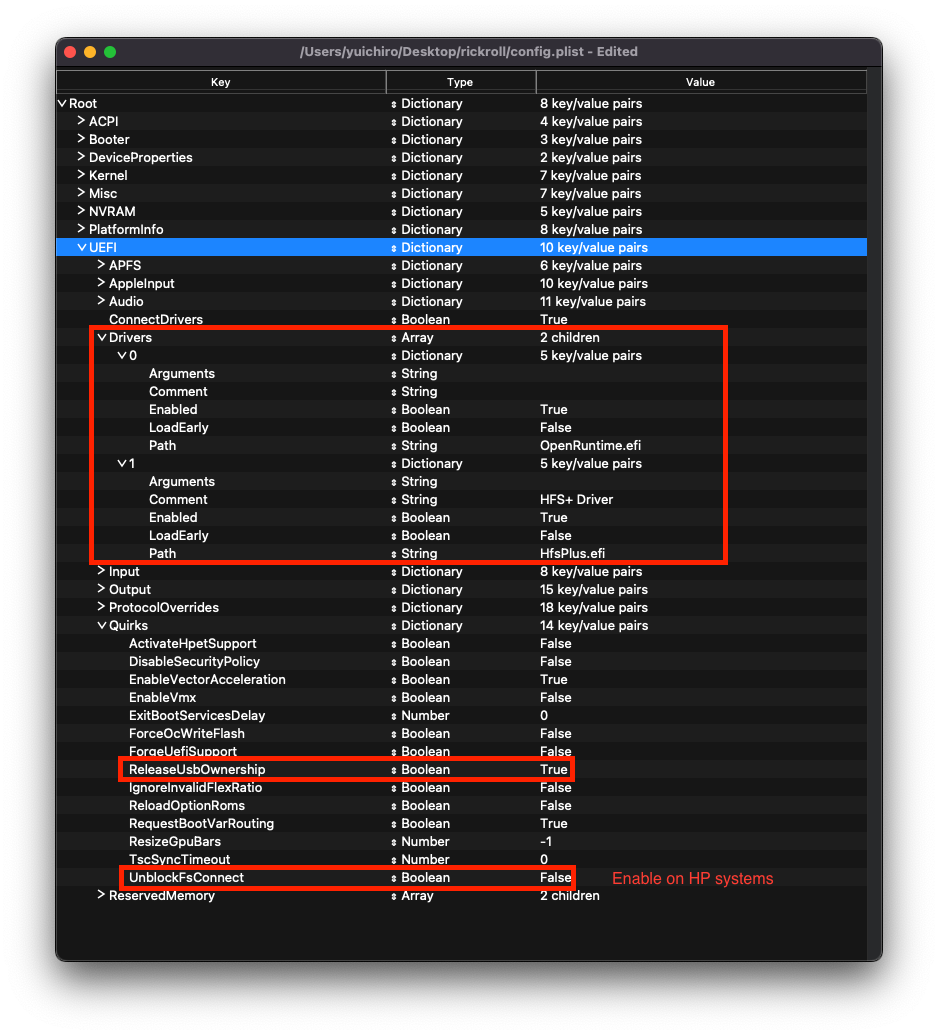
\includegraphics[width=0.8\textwidth]{fotos/PSP/Propertree/UEFI.png}
\break
\emph{Configuring UEFI}
\hfill\break
\hfill\break
Here you don't have to do much only enable ReleaseUsbOwnership, which adds support for USB firmware from laptop vendors. You don't need to enable it but it can be handy if you run garbage laptop vendors like MSI.
\hfill\break
\hfill\break
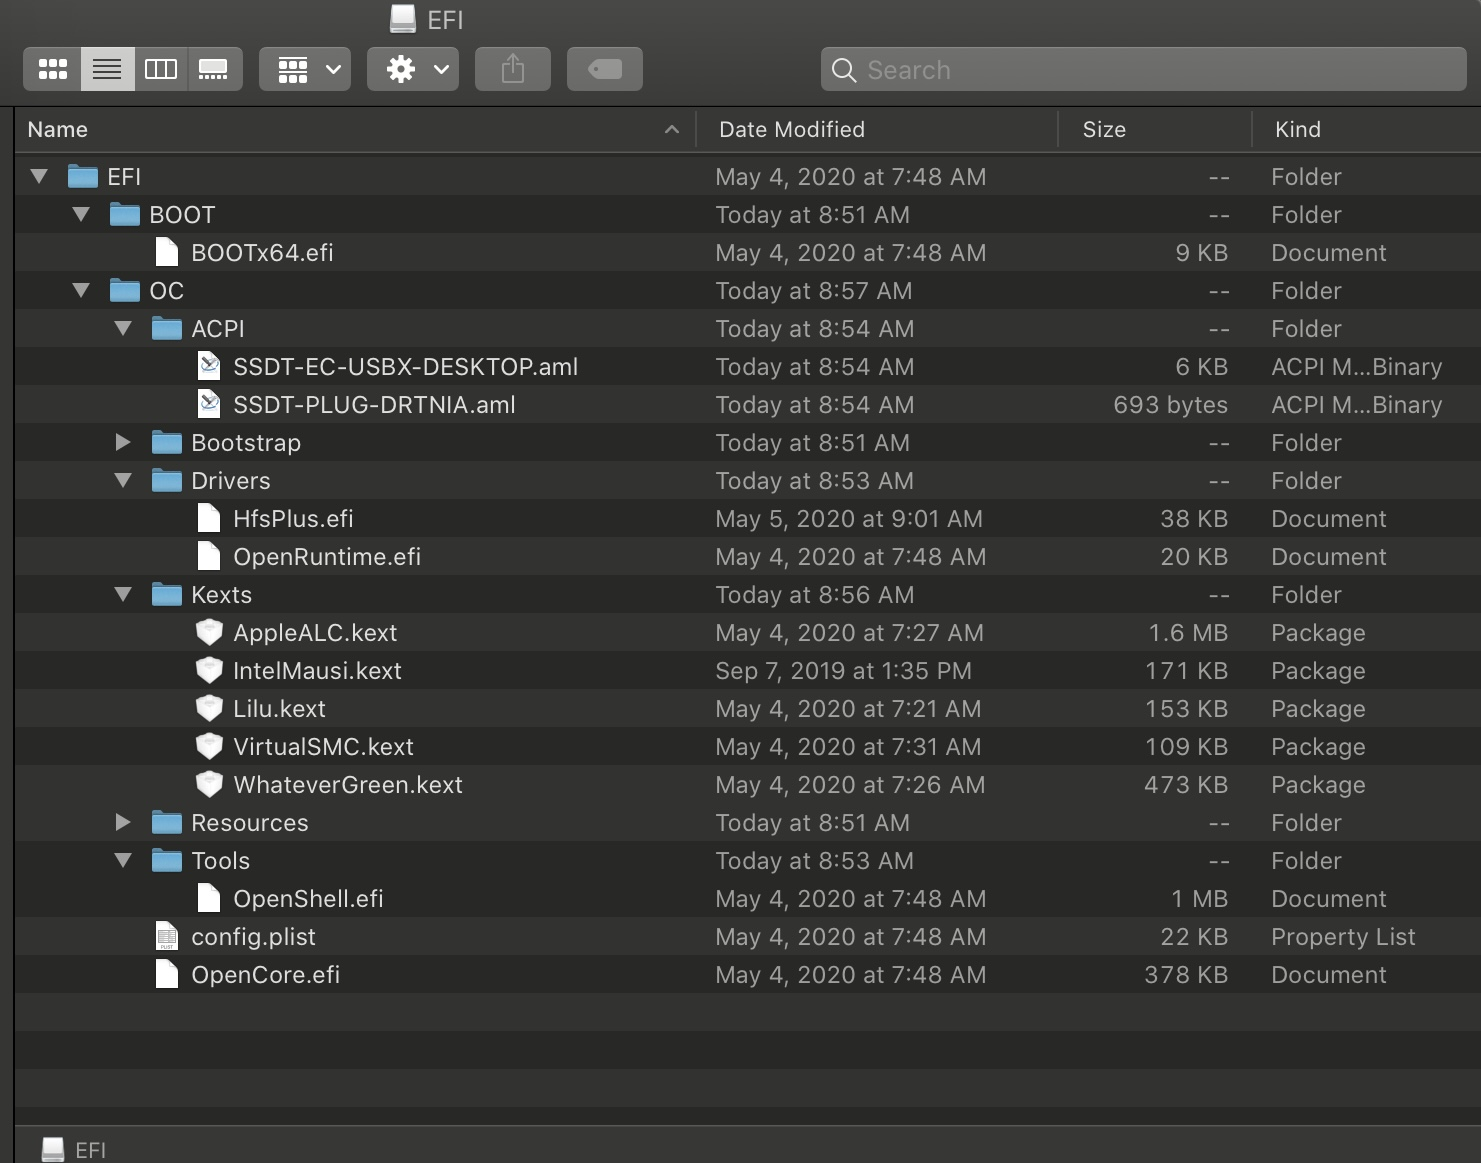
\includegraphics[width=0.8\textwidth]{fotos/PSP/Propertree/Efi preview.jpeg}
\break
\emph{Preview of EFI setup}
\hfill\break
\hfill\break
Once you're done it should look something like this. If you have the same model as I have then my code is online to be used. It works but the HDMI 2.0 has not been patched and my DSDT has not been manually edited to disable my dedicated GPU.
\hfill\break
\hfill\break
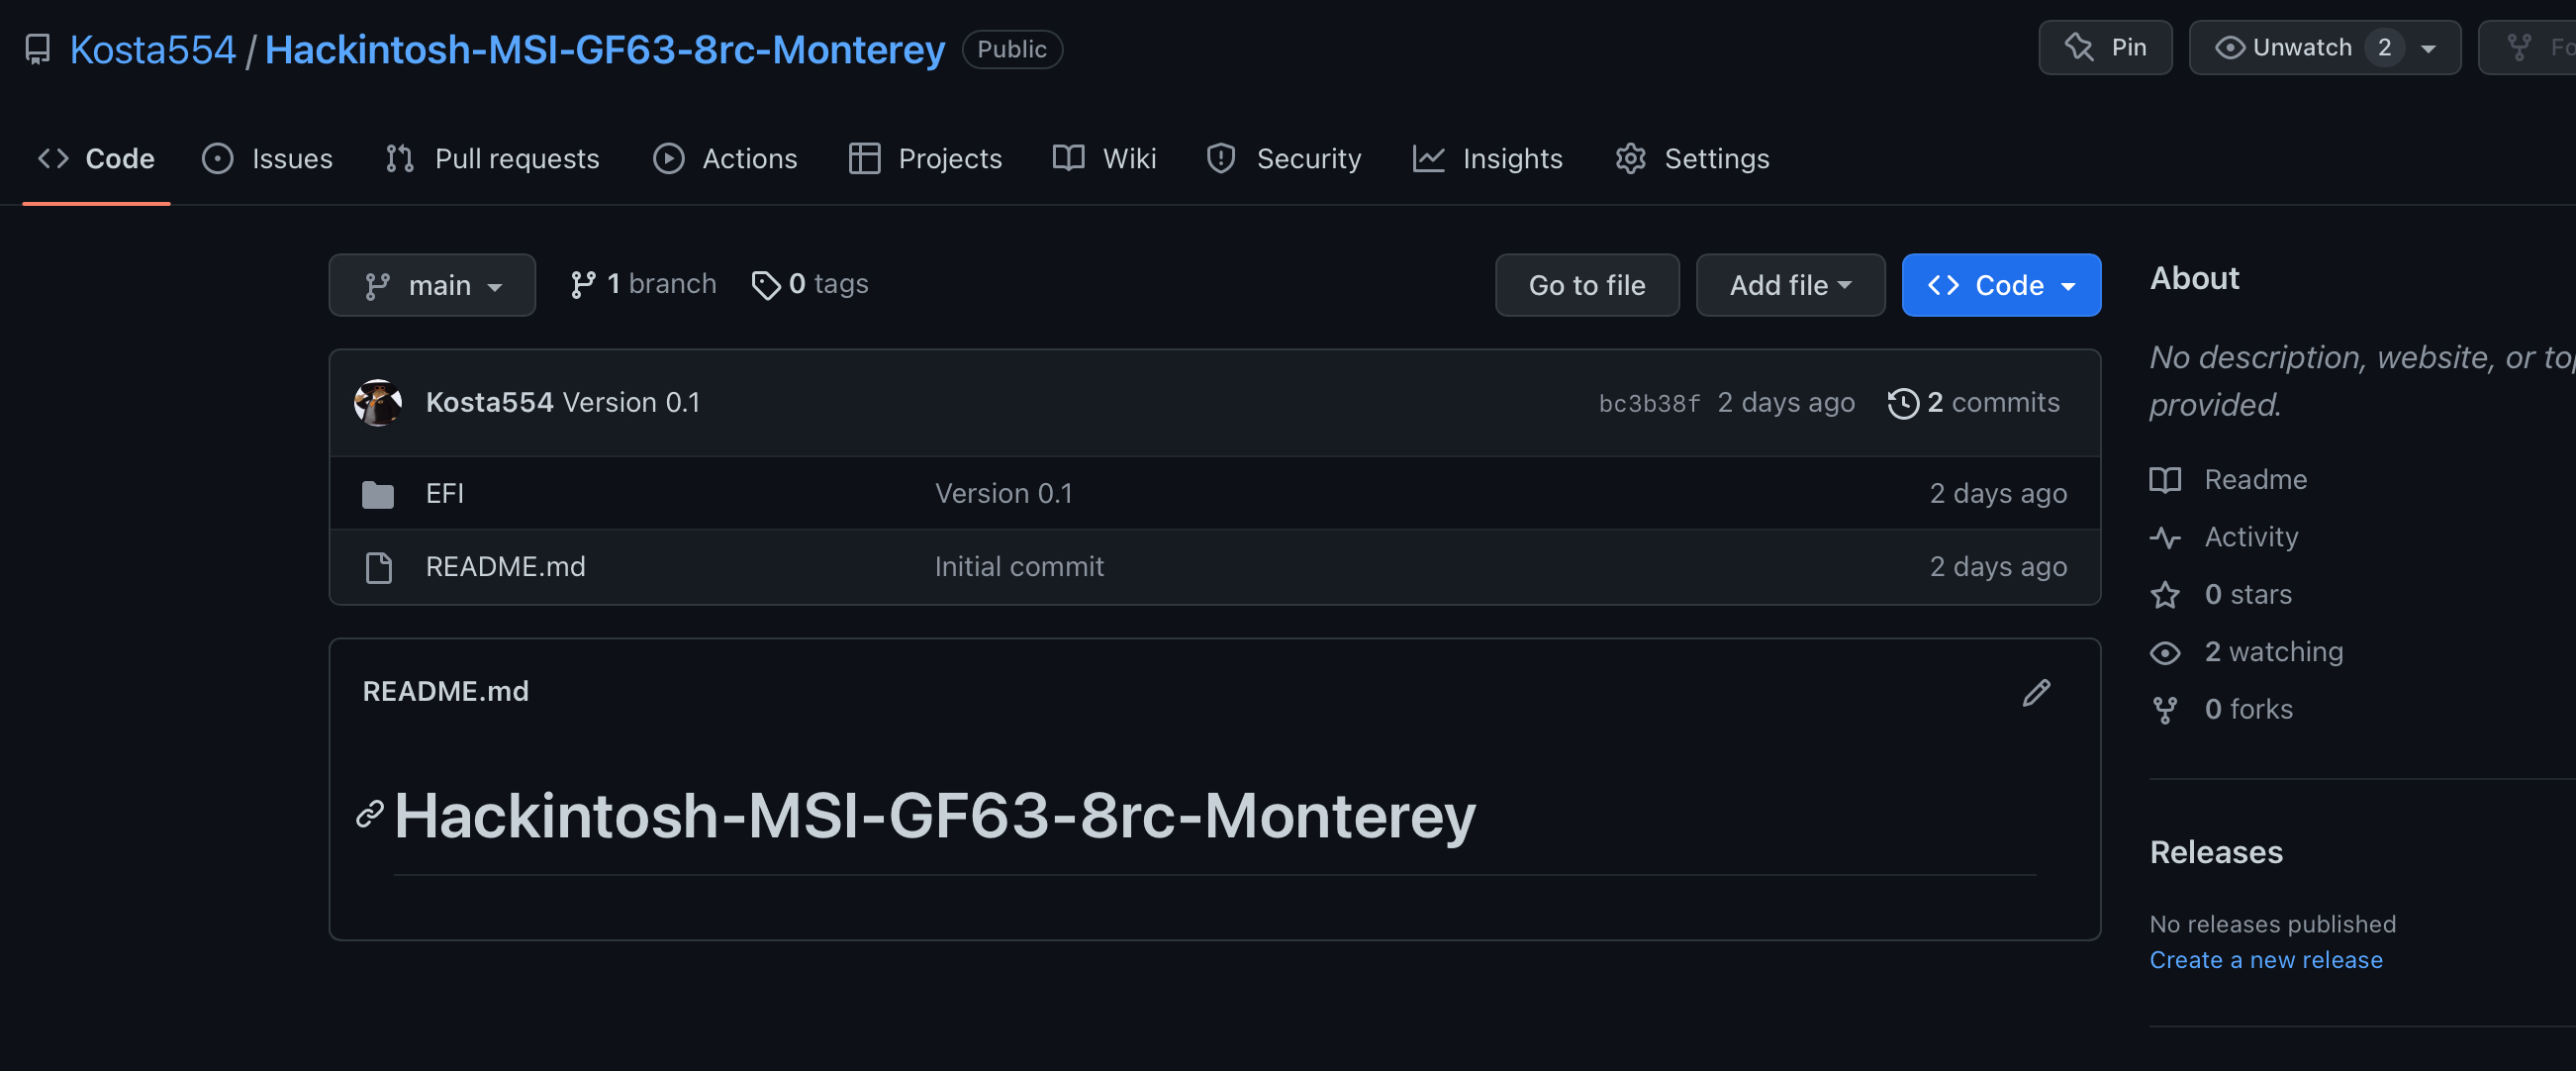
\includegraphics[width=0.8\textwidth]{fotos/PSP/My github.jpeg}
\break
\emph{My compiled config in Github: \url{https://github.com/Kosta554/Hackintosh-MSI-GF63-8rc-Monterey/tree/main}}
\hfill\break
\hfill\break
\subsubsection{Troubleshooting}
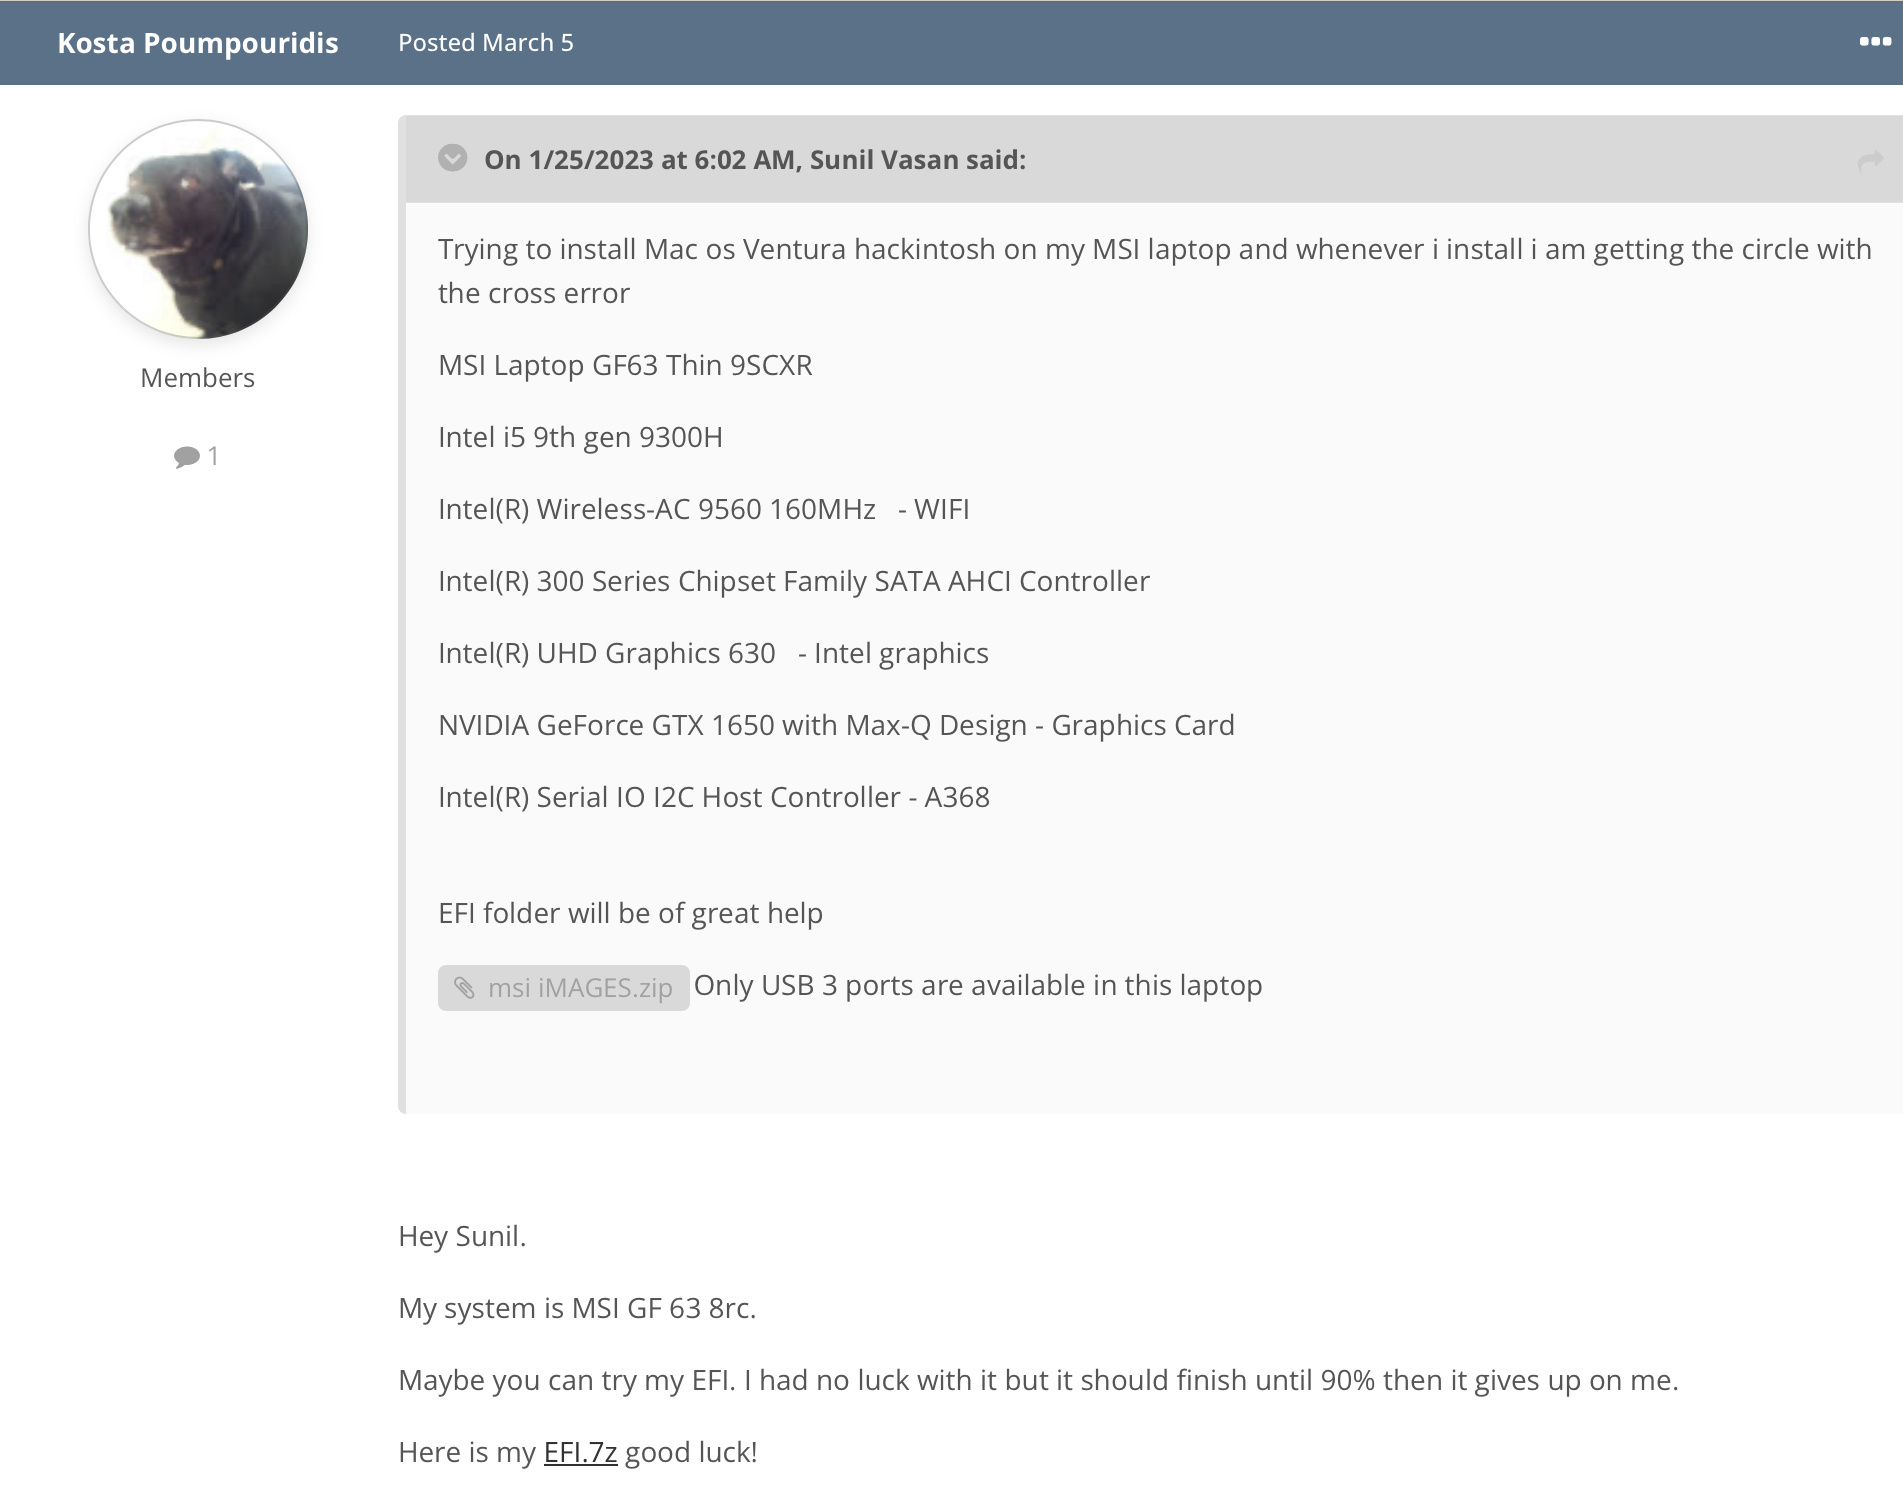
\includegraphics[width=1\textwidth]{fotos/PSP/Research/Oralira post.jpeg}
\break
\emph{Asking a question in one of the Hackintosh forums (Olarila)}
\hfill\break
\hfill\break
As you can see I asked for some help on March 5th and still to this day I did not receive any comment.\hfill\break
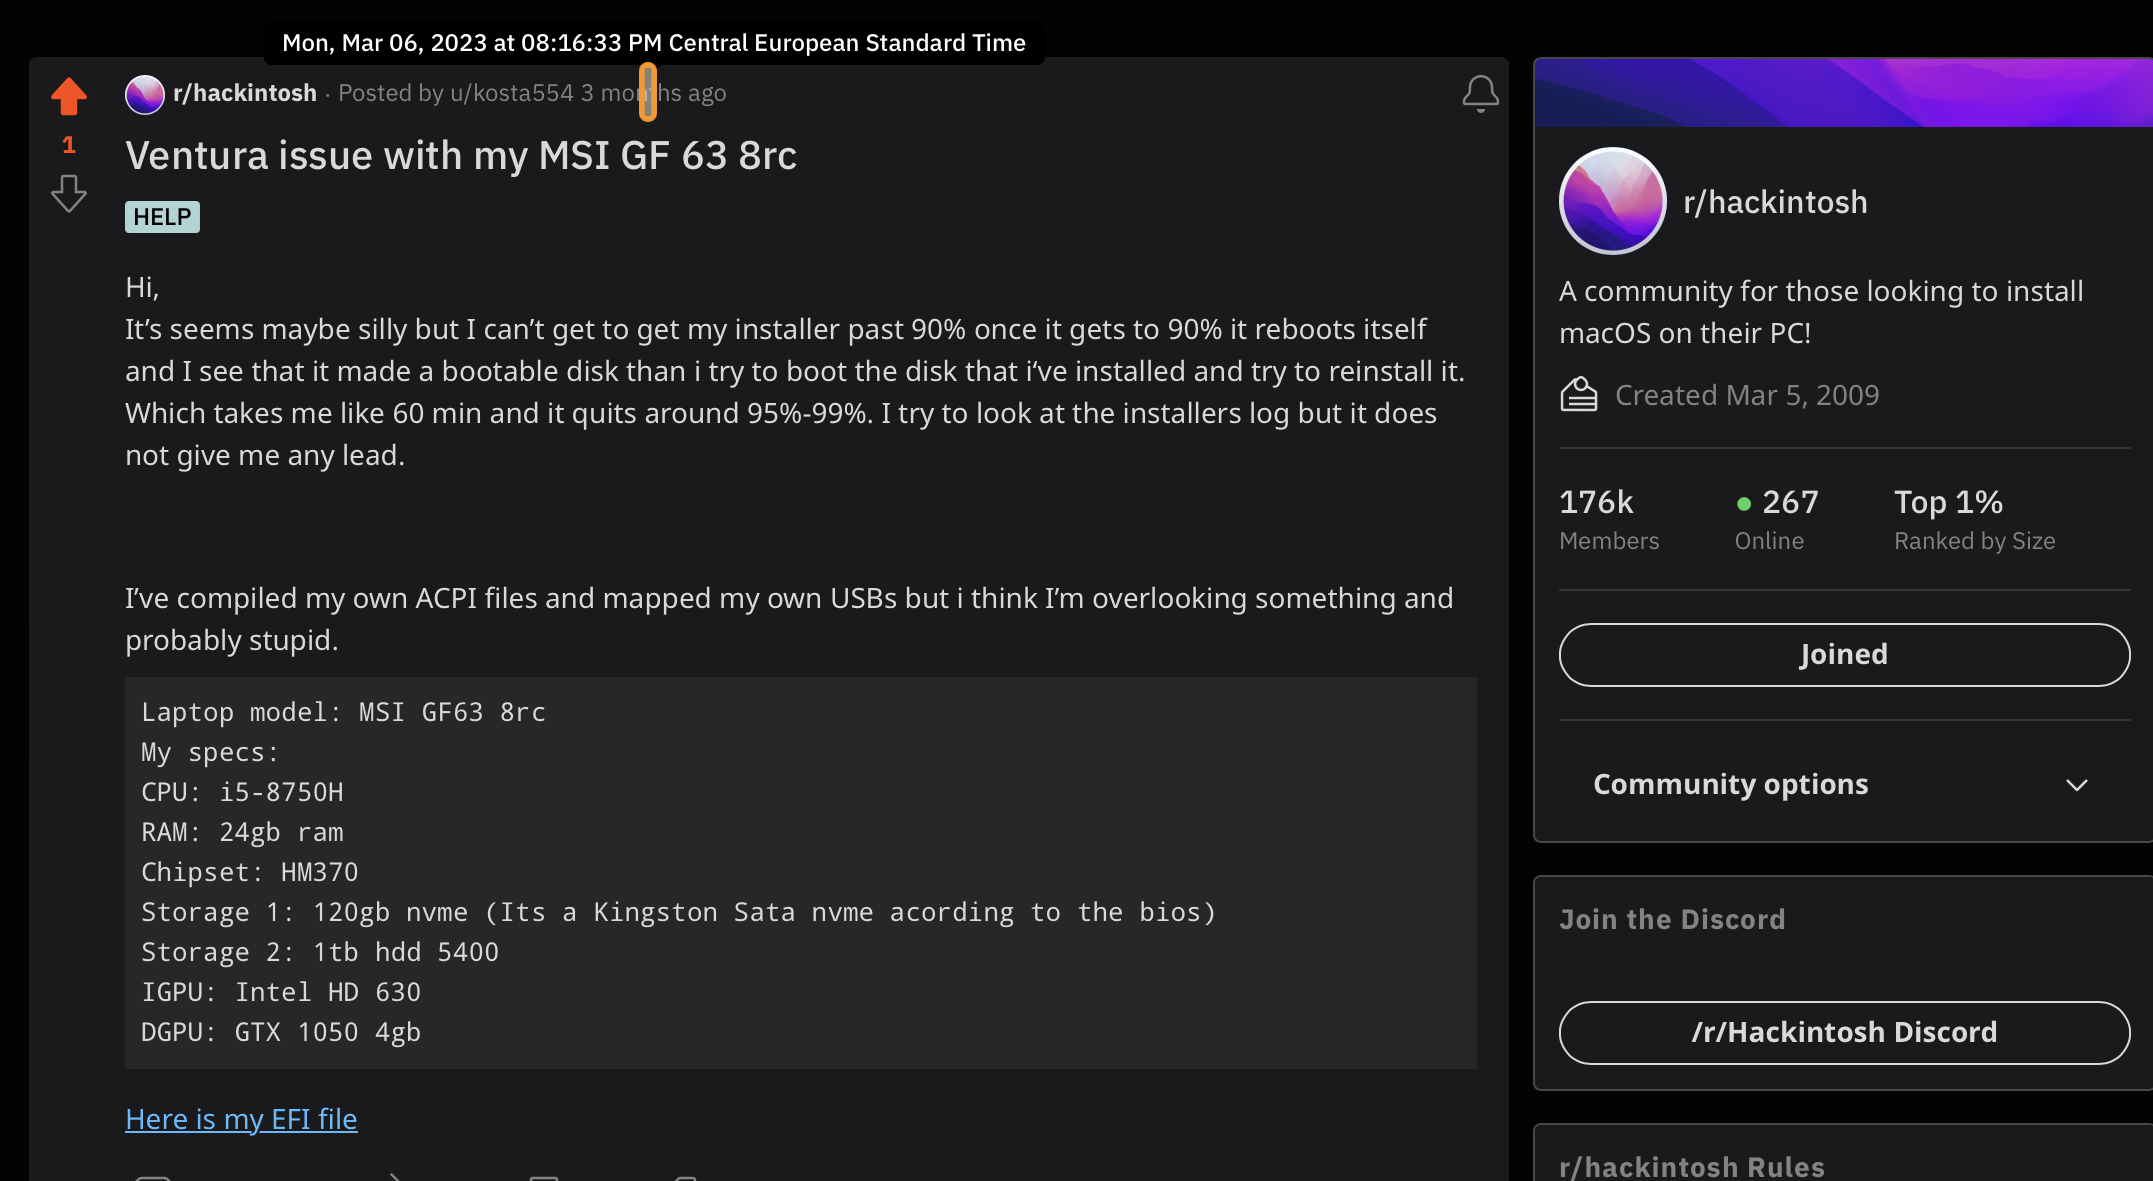
\includegraphics[width=\textwidth]{fotos/PSP/Research/Reddit post.jpeg}
\break
\emph{Asked the same question in Reddit.}
\hfill\break
\hfill\break
Same goes to Reddit I posted it on March 6th and still no comments or anything. I was on my own but now that Reddit is protesting you won't get any answers.
\newpage
\subsection{Testing}


\section{Outcomes}
Here I'll outline the outcomes of my investigation. What I'm hoping to achieve is to identify the exploit and suggest a solution to my classmates.

\subsection{Expected Outcomes}
I've done this earlier on my desktop when it wasn't broken. Eventually was working on my desktop but my pc was 10+ years old so it was compatible with Hackintosh for my laptop, it was a headache or at least I think so since it has NVIDIA GPU and it does not play nice with modern macOS. We will see.

\subsection{Actual Outcomes}
IT WAS A PAIN IN THE ASS to make this work but I could not make it work but it ran back in February but the config does not work anymore and this means I can try and run The macOS Sonoma beta soon which I'm stoked about. But yea it sucks to run natively the best option is to run it on VM or just to buy a Mac. Since I have an iPad Pro I don't need or want to have macOS. 

\hfill\break
\hfill\break
The laptop works half and the install is not the successfully as the version what I had before.
\hfill\break
\hfill\break
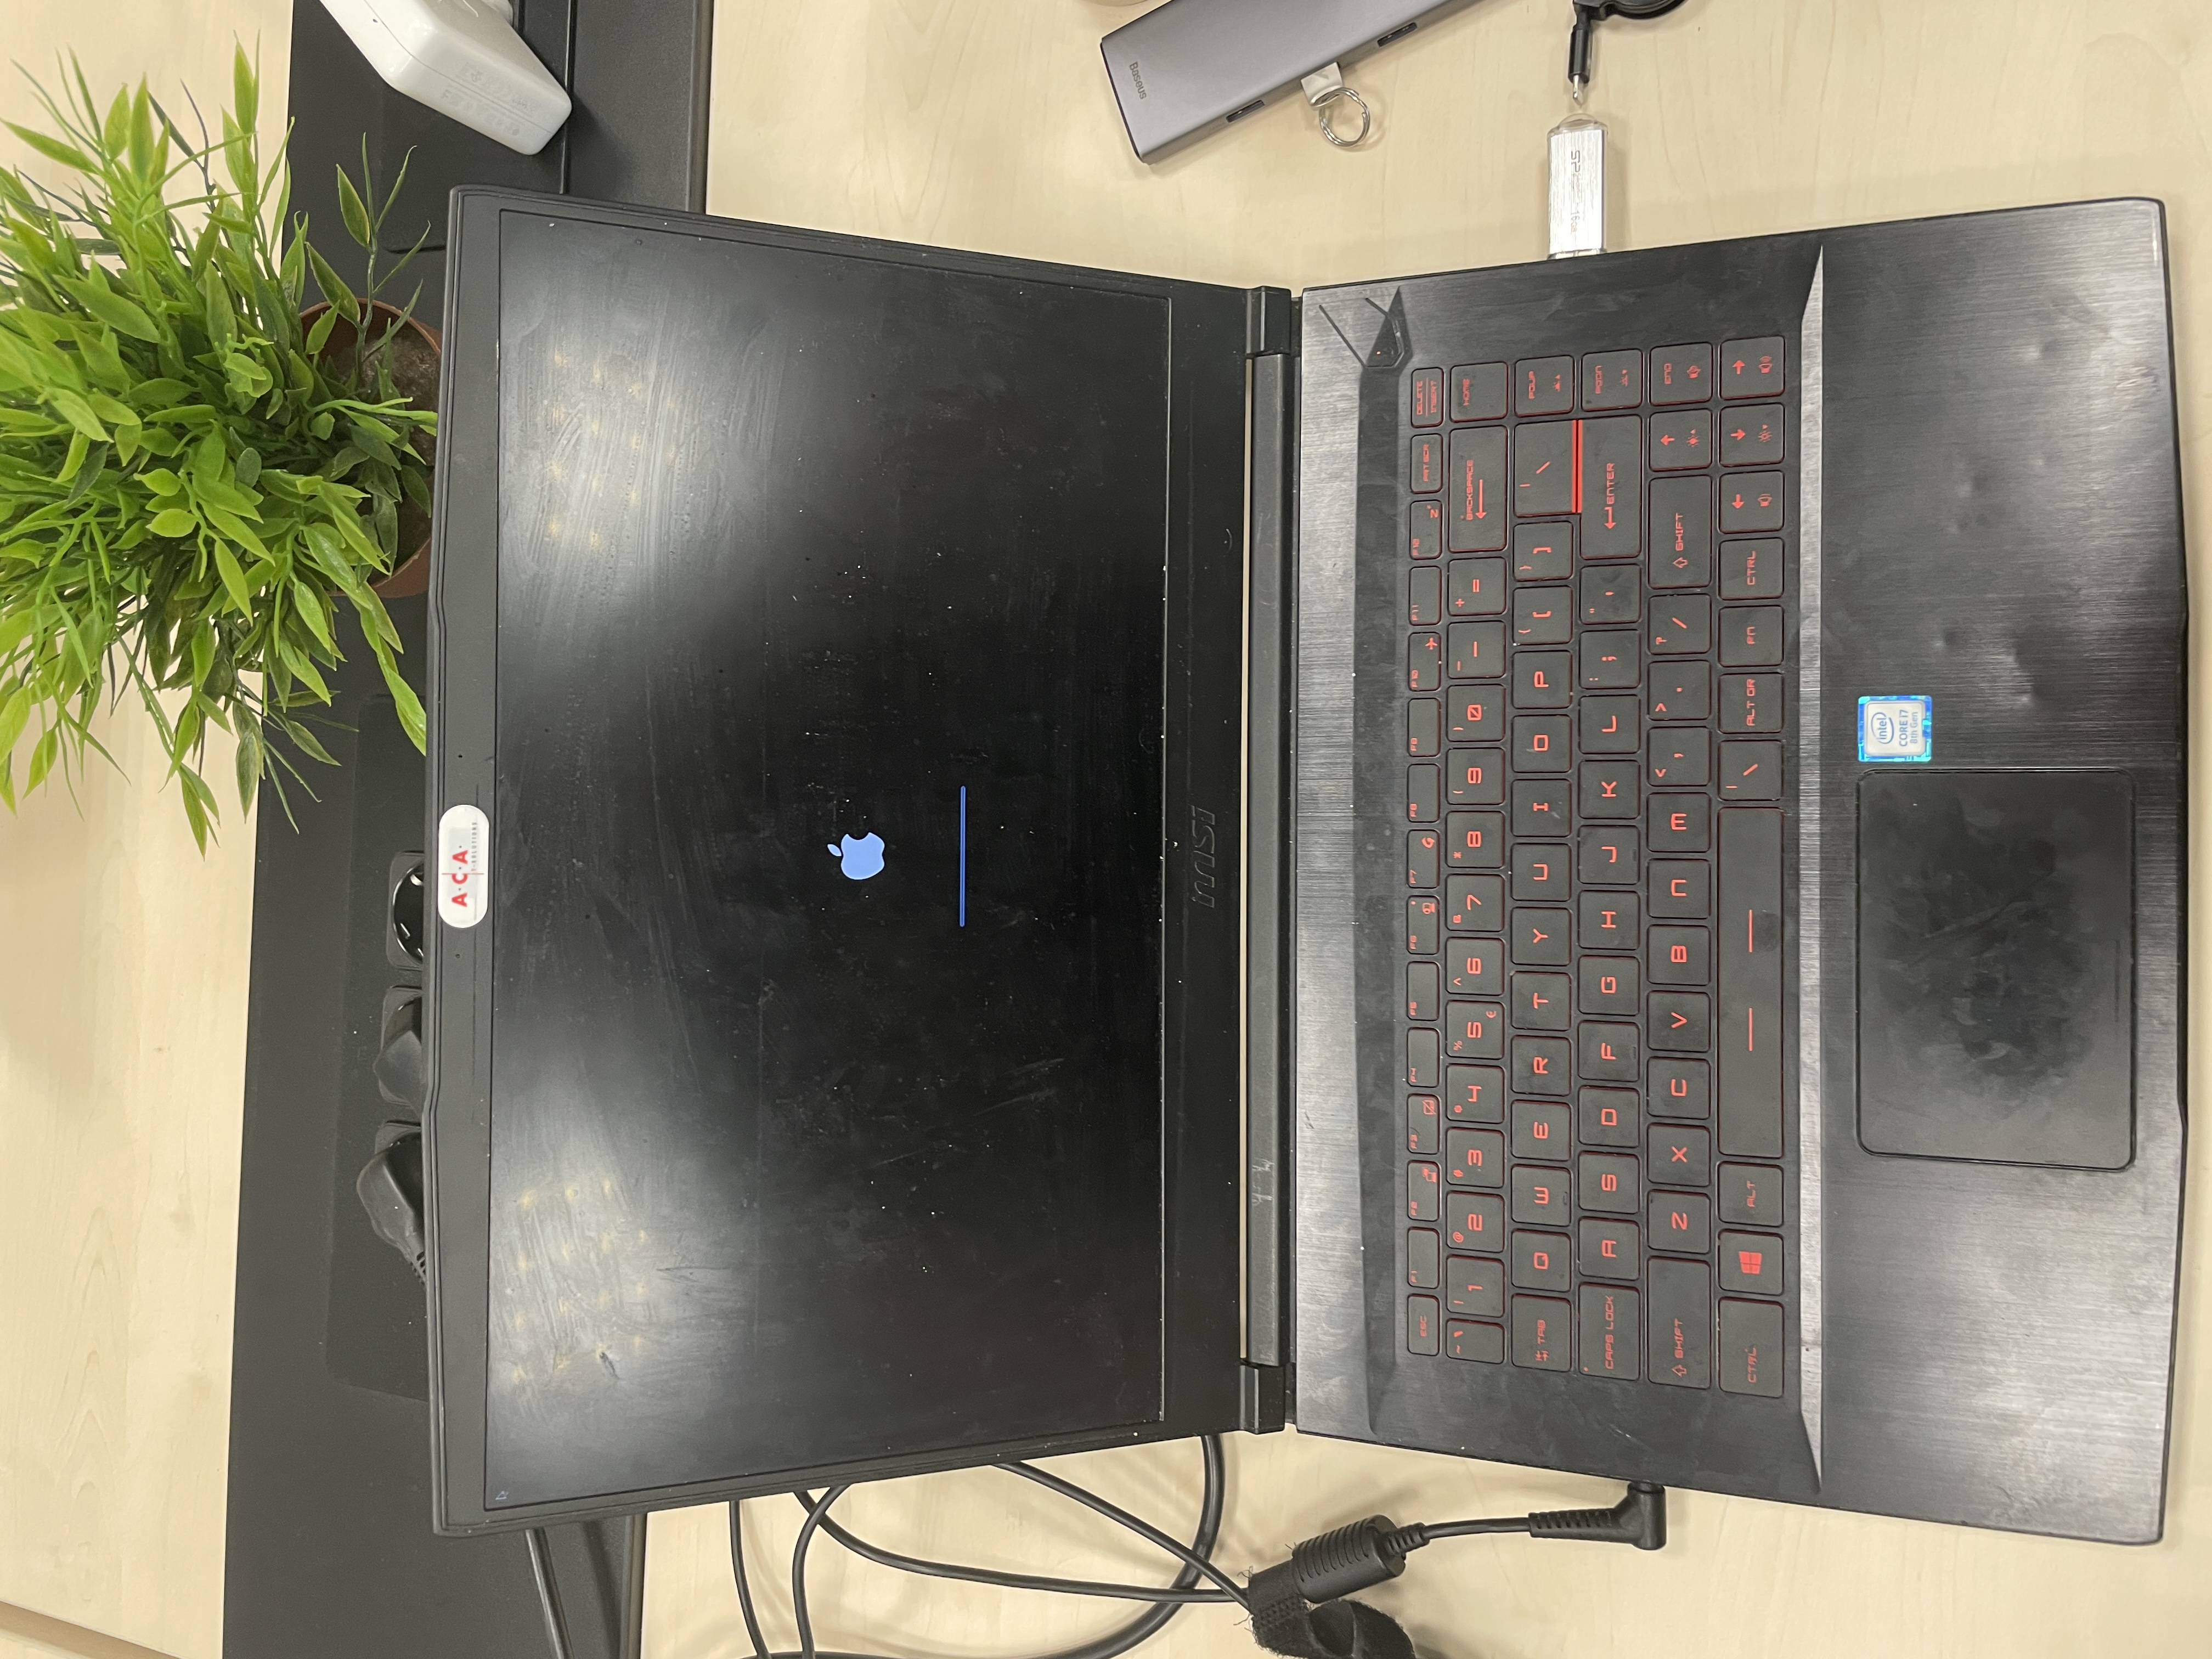
\includegraphics[width=0.8\textwidth]{fotos/PSP/Outcomes/macOS boot.jpeg}
\break
\emph{macOS booting}
\hfill\break
\hfill\break
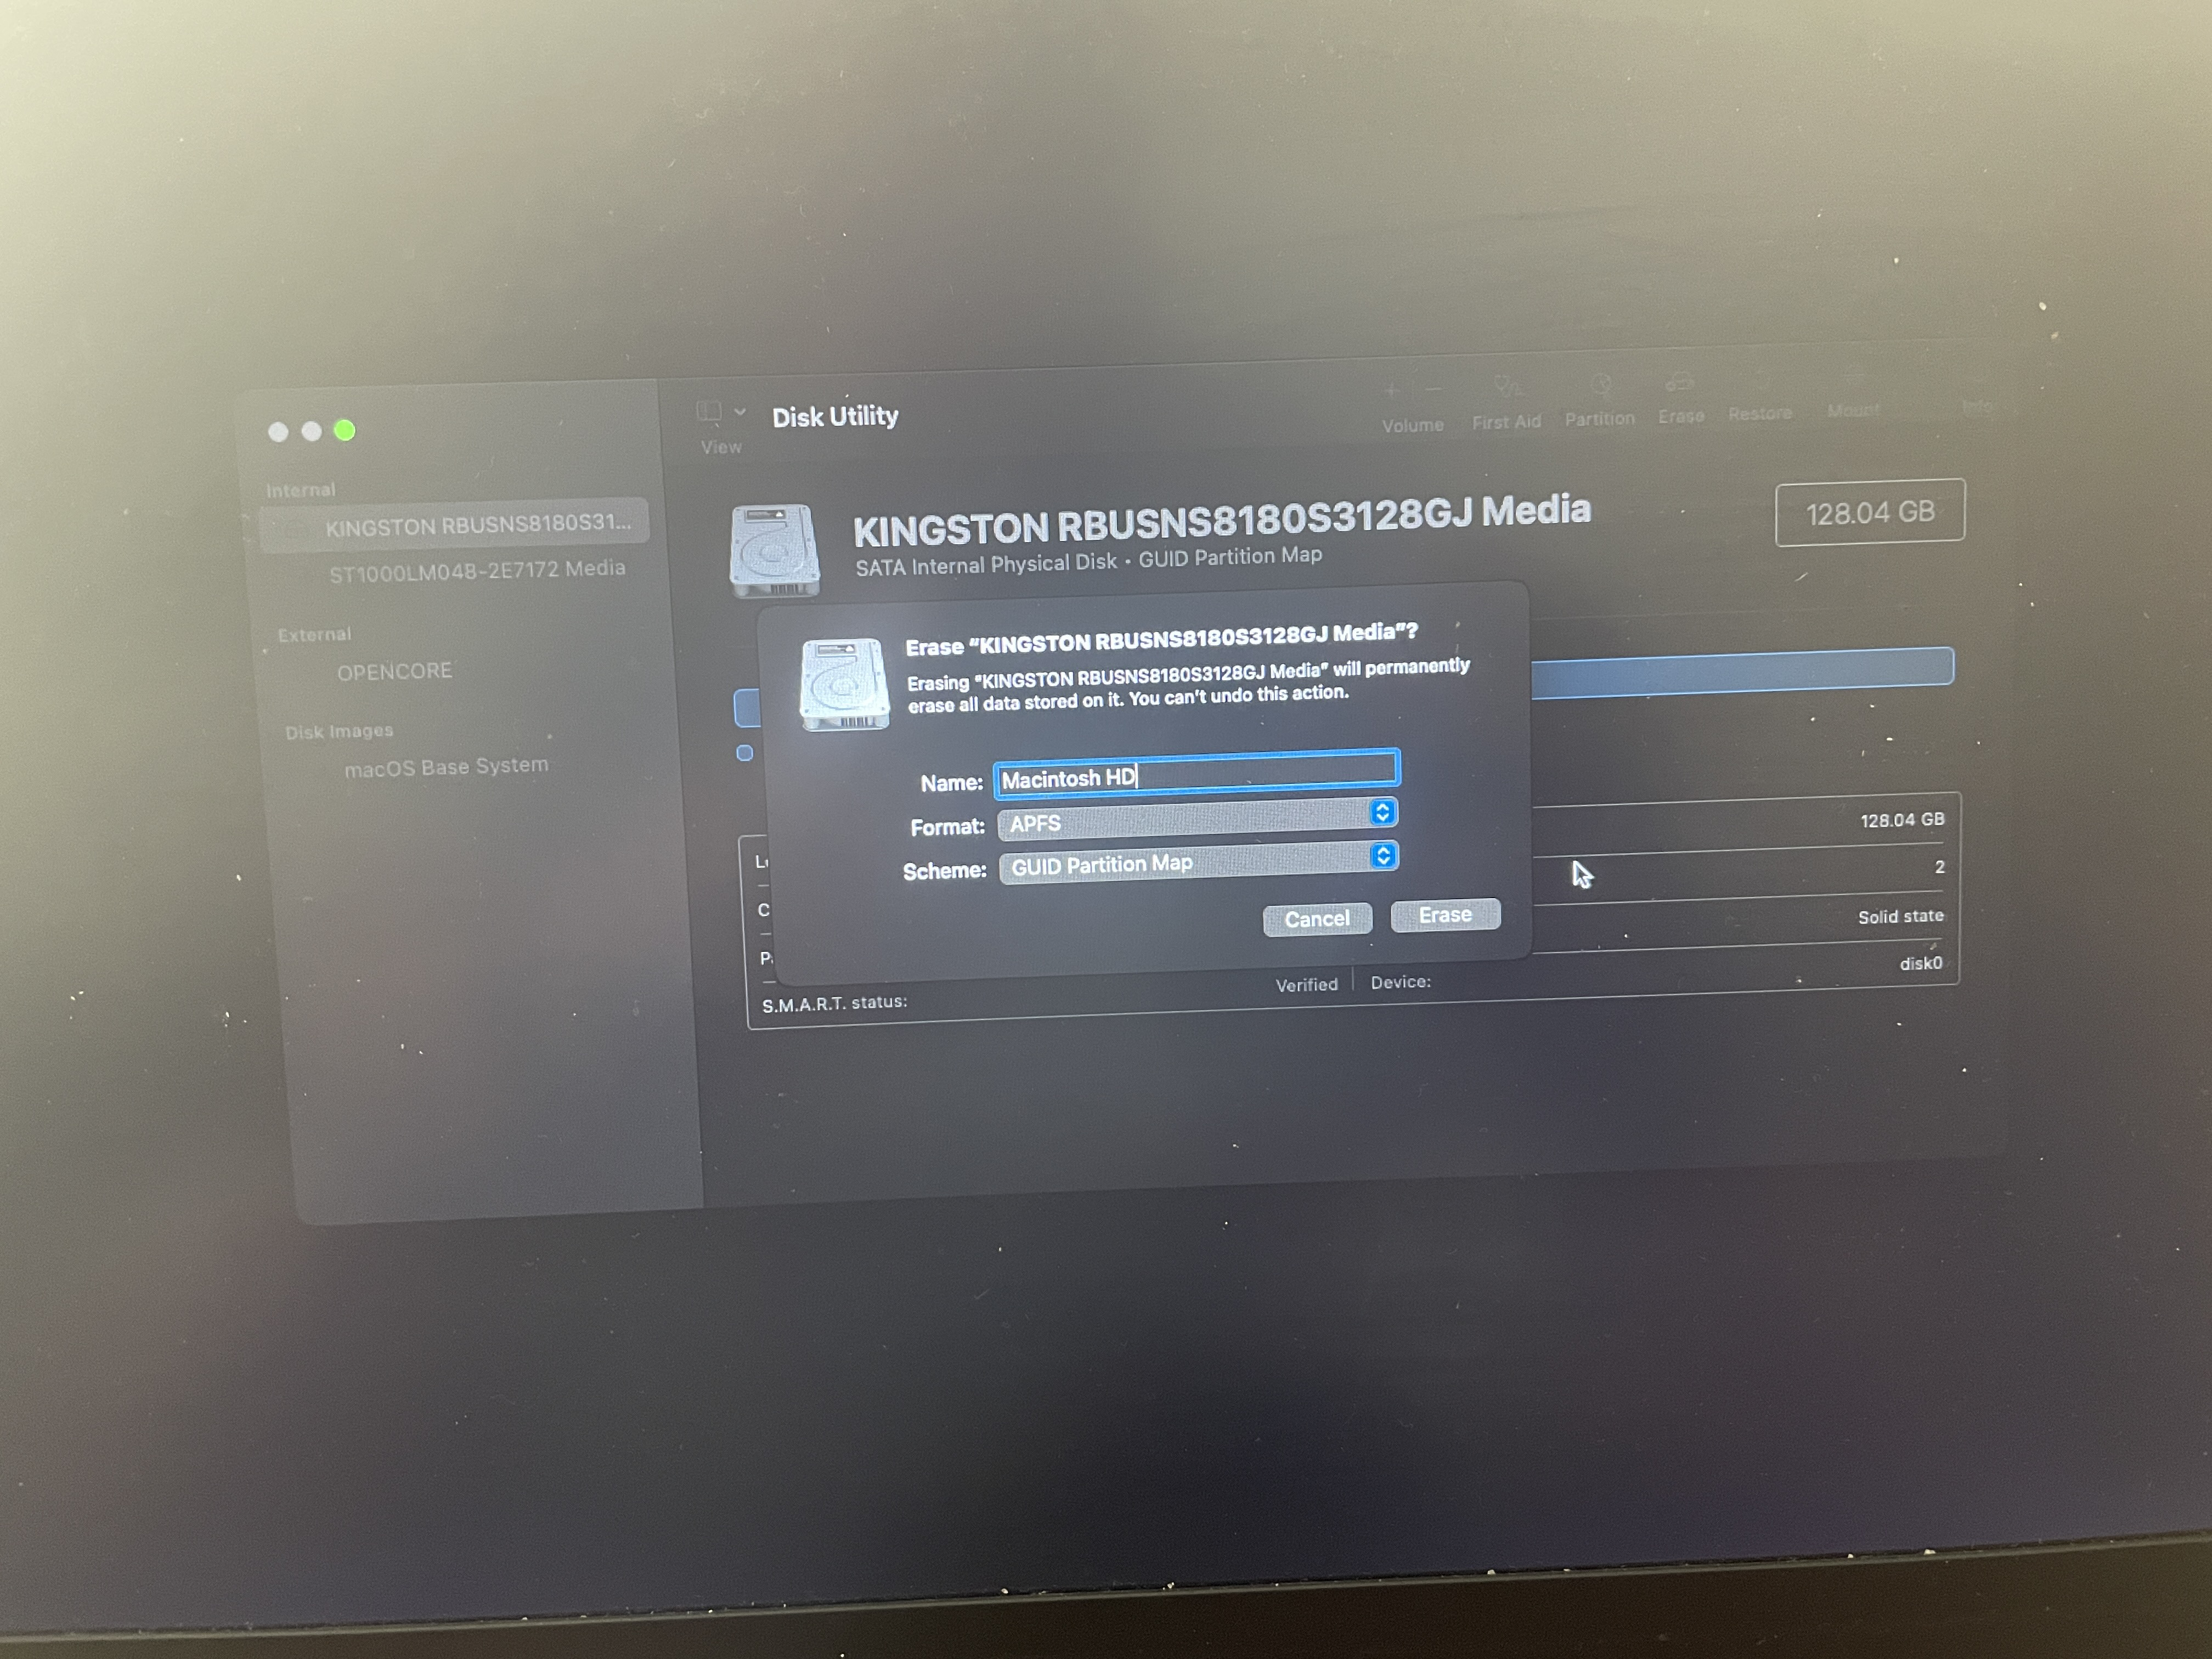
\includegraphics[width=0.8\textwidth]{fotos/PSP/Outcomes/Disc utility macintsohHD.jpeg}
\break
\emph{macOS recovery can see my SSD}
\hfill\break
\hfill\break
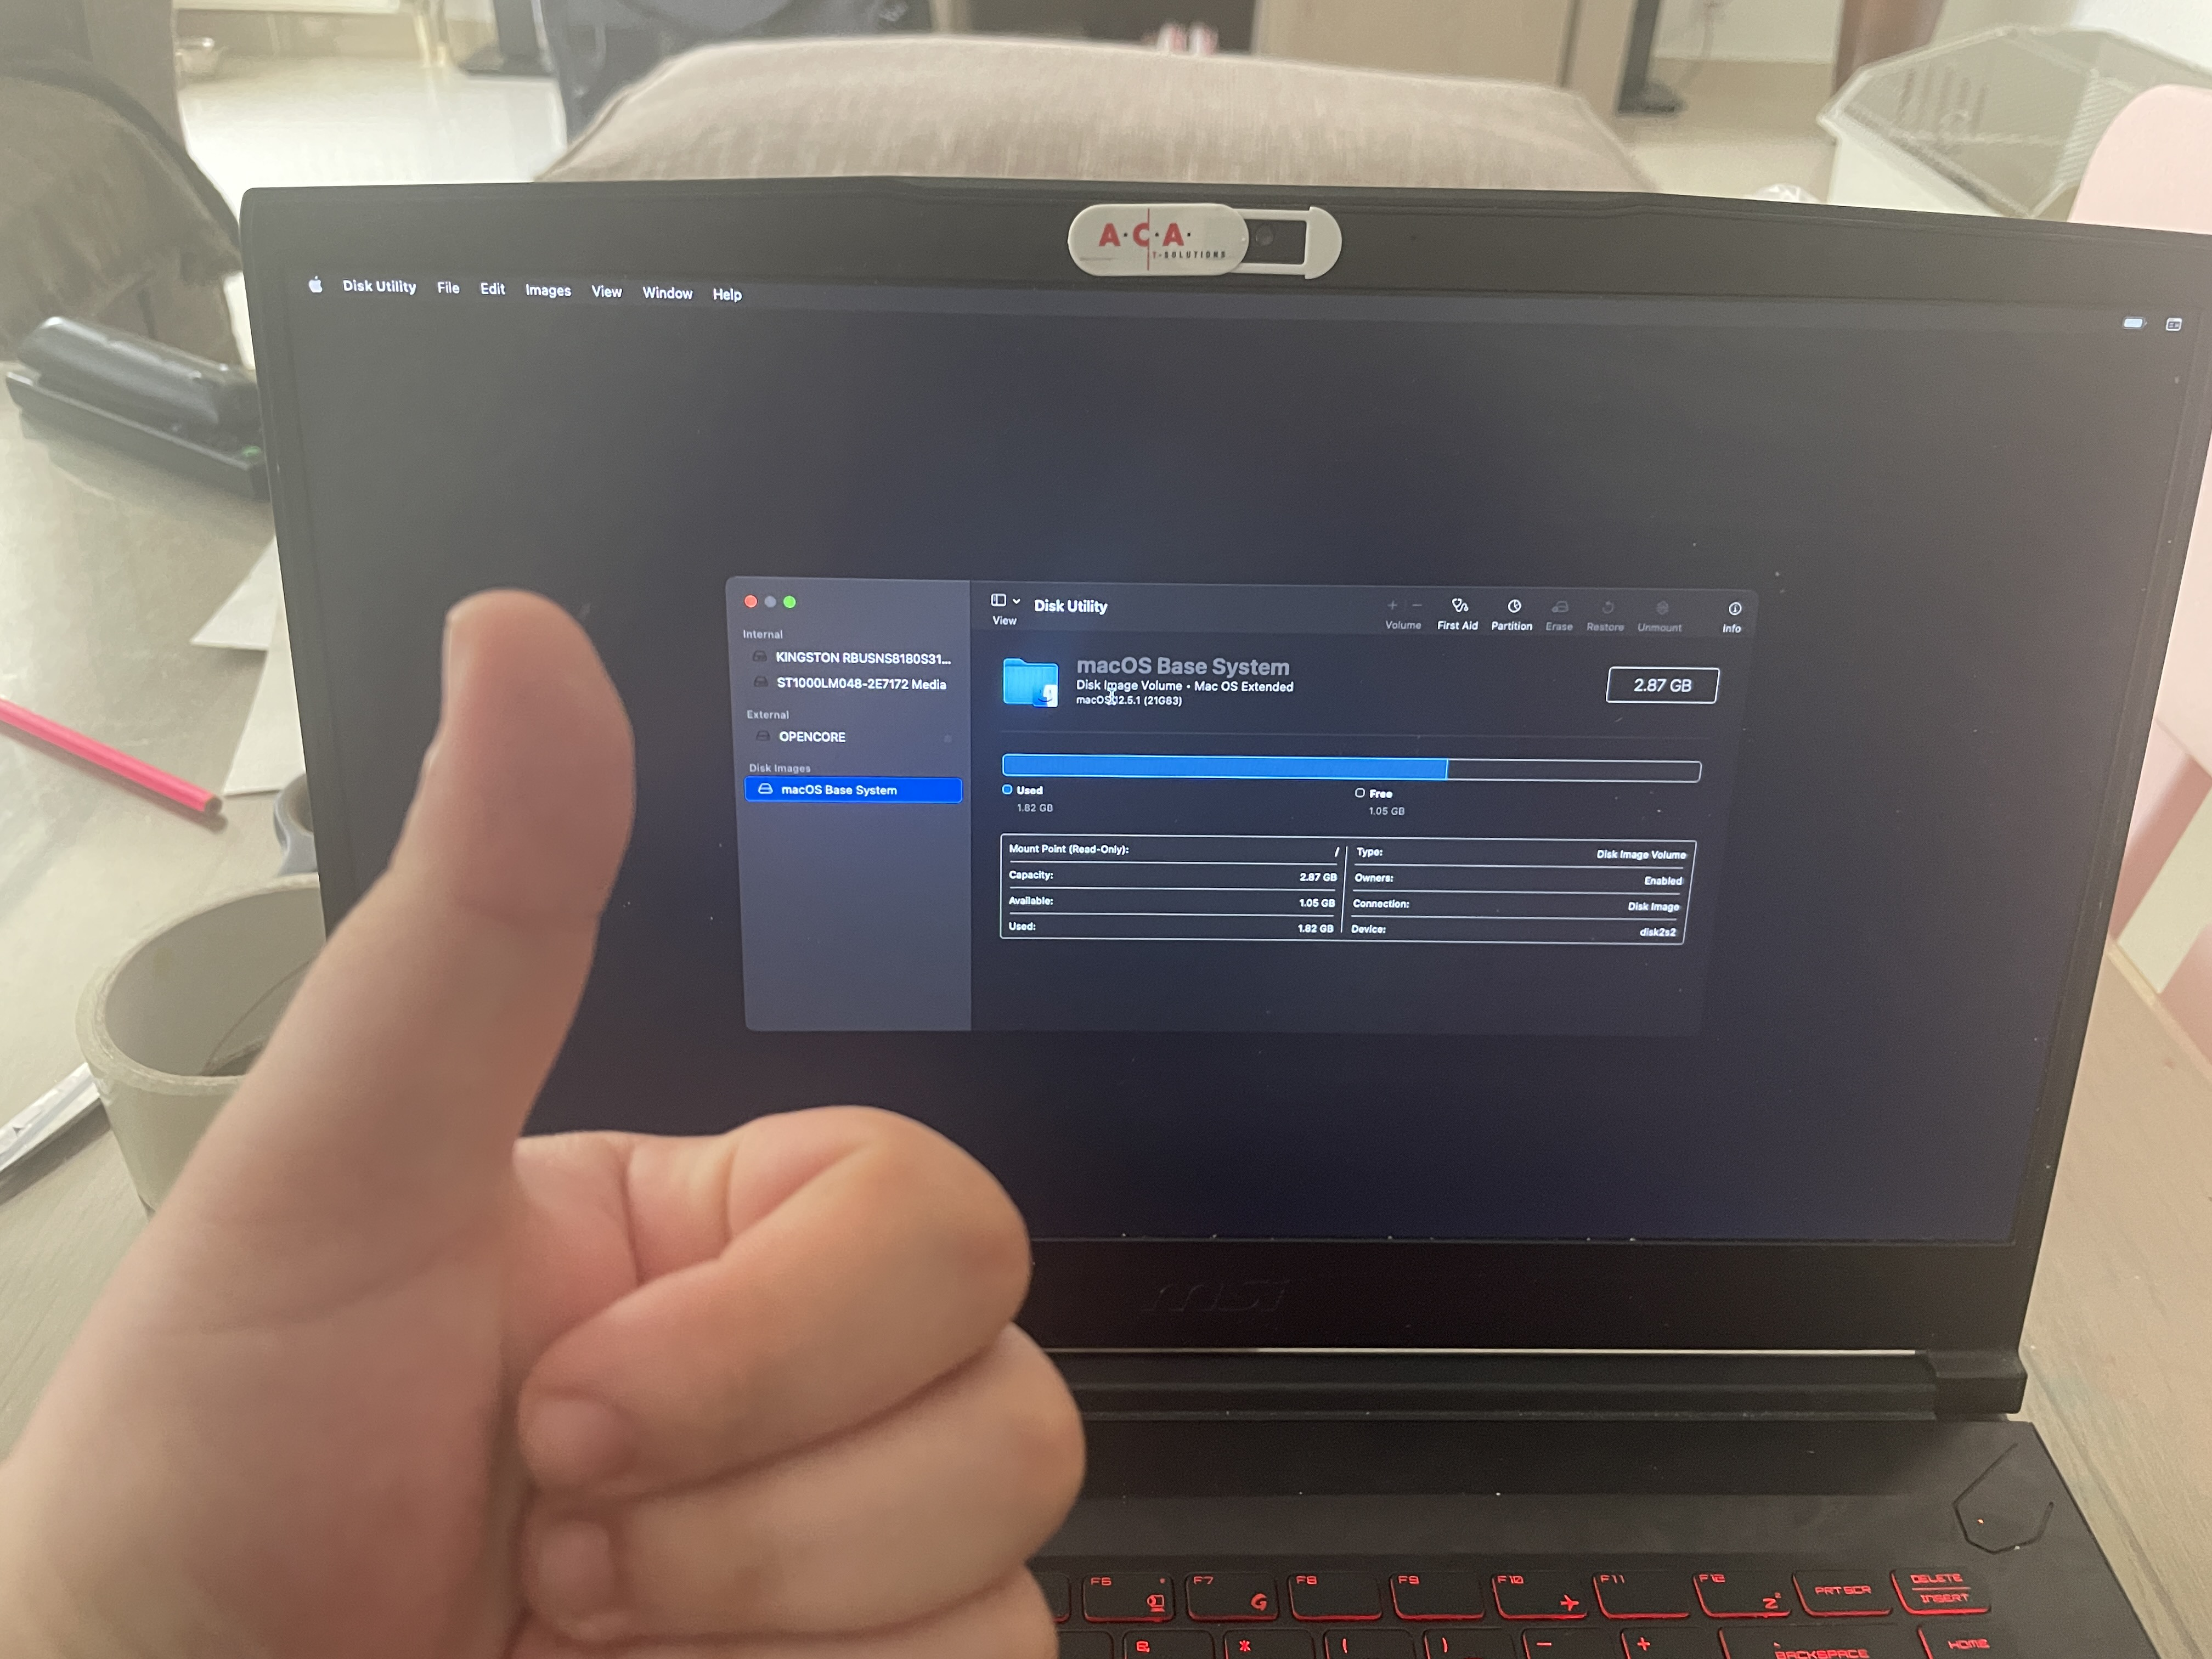
\includegraphics[width=0.8\textwidth]{fotos/PSP/Outcomes/Installer disc utility.jpeg}
\break
\emph{macOS recovery can start partitioning}
\hfill\break
\hfill\break
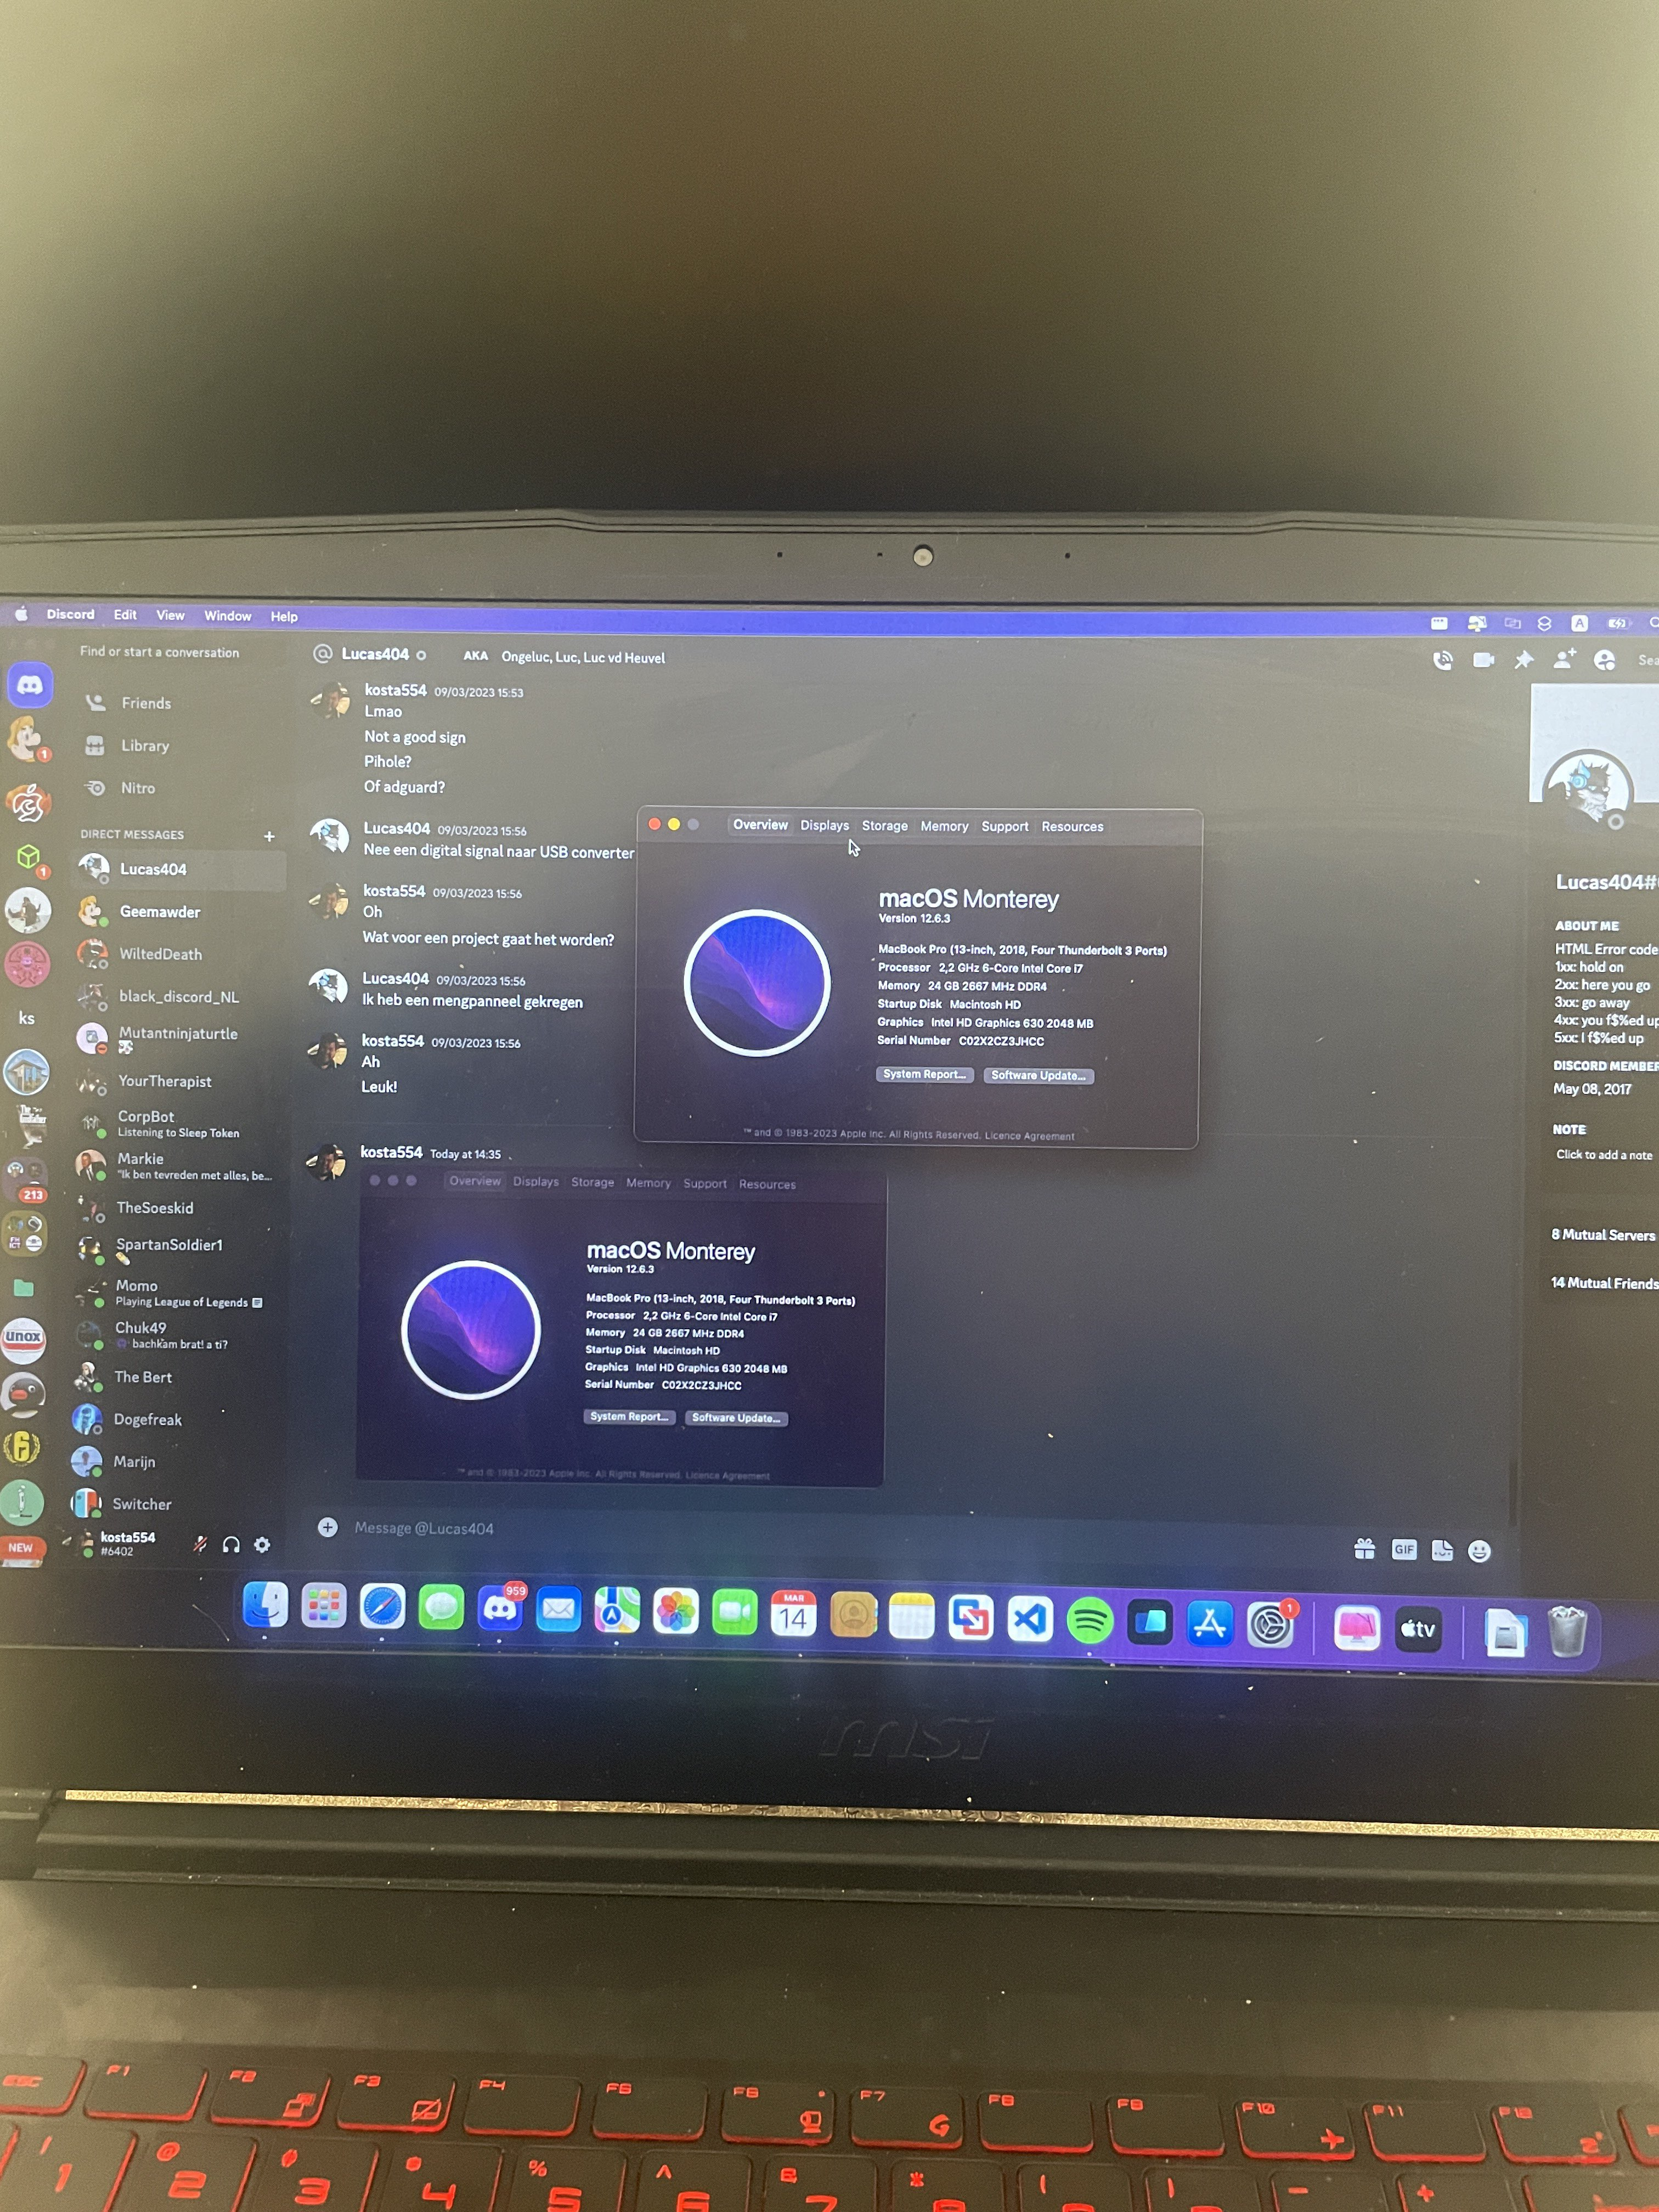
\includegraphics[width=0.8\textwidth]{fotos/PSP/Outcomes/Running macos.jpeg}
\break
\emph{macOS 12 in March}
\newpage
\section{Planning}
In this section I'm going to plan my estimated times:
\hfill\break
    \begin{table}[htbp]
        \begin{tabular}{|l|l|l|}
            \hline
            Estimate Hours & Activity    & Personnel    \tabularnewline \hline
            12 - 19 hours   & Researching about the subject & Kosta \tabularnewline \hline
            4 - 5 hours  & Document my investigation & Kosta \tabularnewline 
            \hline
            20 - 25 hours & Run it in my test environment & Kosta \tabularnewline \hline
            2 - 5 hours & Create Presentation & Kosta \tabularnewline \hline
        \end{tabular}
    \end{table}
\section{In short what I did (TL:DR)}
\textbf{So for TL:DR}
\hfill\break
I had a USB 2.0 16 GB and used Rufus to format in a GPT table partition and copied the open core files alongside my Monterey copy. Now I need to compile my config to my cpu architect (Coffee Lake), plus I need to compile my DSDT (Differentiated System Description Table) so macOS knows how to send instructions to my motherboard and CPU. Once I was done with that I straight up installed all the necessary Kexts and patched my GPU manually. Once that was done I need to spoof my hardware ID with MacBook 15,1. And after that, it is just trial and error until it boots and installs.
\section{Conclusion}
In conclusion. If you want to run macOS just buy a MAC and save yourself some hassle. If you really don't want to buy one then the best solution is to run it through a server or use KVM PCI passthrough since you can spoof all the components and it is future-proof because it can emulate ARM architecture, at least they are working on it. We are in the middle of an architect transition because Intel is creating a new x86 architecture (x86-s) and people are dipping into ARM like AMD, Intel, Qualcomm, Apple, MediaTek and Microsoft for desktops and laptops.
\hfill\break
\hfill\break
Also, note that I made this earlier in February but forgot to make a backup of a working macOS that runs and has iMessage and Facetime active.

\subsection{About the Research Questions}
Compared to genuine Mac devices they have the advantage that computers are expandable and upgradeable which Macs arent. Second is that the cheapest laptops can run macOS, I wouldn't recommend that but it is possible. and last because people like macOS and they don't want to buy a device to run an operating system.

\end{document}
